% ******************************************************************************
% ******************************* BEGIN DOCUMENT *******************************
% ******************************************************************************
%\documentclass[a4paper,12pt,twoside,online,customfont,custombib,PageStyleI,draftclassic]{Settings/PhDThesisPSnPDF}
\documentclass[a4paper,12pt,twoside,customfont,custombib,PageStyleI]{Settings/PhDThesisPSnPDF}

% ********************************** Preamble **********************************
% Preamble: Contains packages and user-defined commands and settings
% ******************************************************************************
% ****************************** Custom Margin *********************************

% Add `custommargin' in the document class options to use this section
% Set {innerside margin / outerside margin / topmargin / bottom margin}  and
% other page dimensions
\ifsetCustomMargin
  \RequirePackage[left=37mm,right=30mm,top=35mm,bottom=30mm]{geometry}
  \setFancyHdr % To apply fancy header after geometry package is loaded
\fi

% Add spaces between paragraphs
%\setlength{\parskip}{0.5em}
% Ragged bottom avoids extra whitespaces between paragraphs
\raggedbottom
% To remove the excess top spacing for enumeration, list and description
%\usepackage{enumitem}
%\setlist[enumerate,itemize,description]{topsep=0em}

% *****************************************************************************
% ******************* Fonts (like different typewriter fonts etc.)*************

% Add `customfont' in the document class option to use this section

\ifsetCustomFont
  % Set your custom font here and use `customfont' in options. Leave empty to
  % load computer modern font (default LaTeX font).
  \RequirePackage{palatino}

  % For use with XeLaTeX
  %  \setmainfont[
  %    Path              = ./libertine/opentype/,
  %    Extension         = .otf,
  %    UprightFont = LinLibertine_R,
  %    BoldFont = LinLibertine_RZ, % Linux Libertine O Regular Semibold
  %    ItalicFont = LinLibertine_RI,
  %    BoldItalicFont = LinLibertine_RZI, % Linux Libertine O Regular Semibold Italic
  %  ]
  %  {libertine}
  %  % load font from system font
  %  \newfontfamily\libertinesystemfont{Linux Libertine O}
\fi

% *****************************************************************************
% **************************** Custom Packages ********************************

% ************************* Algorithms and Pseudocode **************************

%\usepackage{algpseudocode}


% ********************Captions and Hyperreferencing / URL **********************

% Captions: This makes captions of figures use a boldfaced small font.
%\RequirePackage[small,bf]{caption}

\RequirePackage[labelsep=space,tableposition=top]{caption}
\renewcommand{\figurename}{Fig.} %to support older versions of captions.sty

\definecolor{BrightLightBlue}{RGB}{51, 153, 255} %bright light blue
\hypersetup{
    colorlinks=true,
    linkcolor=blue,
    filecolor=blue,      
    urlcolor=BrightLightBlue, 
    citecolor=blue,
    pdfpagemode=FullScreen}

% *************************** Graphics and figures *****************************

%\usepackage{rotating}
%\usepackage{wrapfig}

% Uncomment the following two lines to force Latex to place the figure.
% Use [H] when including graphics. Note 'H' instead of 'h'
%\usepackage{float}
%\restylefloat{figure}

% Subcaption package is also available in the sty folder you can use that by
% uncommenting the following line
% This is for people stuck with older versions of texlive
%\usepackage{sty/caption/subcaption}
\usepackage{subcaption}

% ********************************** Tables ************************************
\usepackage{booktabs} % For professional looking tables
\usepackage{multirow}

%\usepackage{multicol}
%\usepackage{longtable}
%\usepackage{tabularx}


% *********************************** SI Units *********************************
\usepackage{siunitx} % use this package module for SI units
\AtBeginDocument{\RenewCommandCopy\qty\SI}
\ExplSyntaxOn
\msg_redirect_name:nnn { siunitx } { physics-pkg } { none }
\ExplSyntaxOff


% ******************************* Line Spacing *********************************

% Choose linespacing as appropriate. Default is one-half line spacing as per the
% University guidelines

% \doublespacing
% \onehalfspacing
% \singlespacing


% ************************ Formatting / Footnote *******************************

% Don't break enumeration (etc.) across pages in an ugly manner (default 10000)
%\clubpenalty=500
%\widowpenalty=500

%\usepackage[perpage]{footmisc} %Range of footnote options


% *****************************************************************************
% *************************** Bibliography  and References ********************

%\usepackage{cleveref} %Referencing without need to explicitly state fig /table

% Add `custombib' in the document class option to use this section
\ifuseCustomBib
  % \RequirePackage[square, sort, numbers, authoryear]{natbib} % CustomBib

% If you would like to use biblatex for your reference management, as opposed to the default `natbibpackage` pass the option `custombib` in the document class. Comment out the previous line to make sure you don't load the natbib package. Uncomment the following lines and specify the location of references.bib file

\RequirePackage[backend=biber, style=numeric-comp, citestyle=numeric, sorting=nty, natbib=true]{biblatex}
\bibliography{bibliography.bib} %Location of references.bib only for biblatex

\fi

% changes the default name `Bibliography` -> `References'
\renewcommand{\bibname}{References}


% ******************************** Roman Pages *********************************
% The romanpages environment set the page numbering to lowercase roman one
% for the contents and figures lists. It also resets
% page-numbering for the remainder of the dissertation (arabic, starting at 1).

\newenvironment{romanpages}{
  \setcounter{page}{1}
  \renewcommand{\thepage}{\roman{page}}}
{\newpage\renewcommand{\thepage}{\arabic{page}}}


% ******************************************************************************
% ************************* User Defined Commands ******************************
% ******************************************************************************

% *********** To change the name of Table of Contents / LOF and LOT ************

%\renewcommand{\contentsname}{My Table of Contents}
%\renewcommand{\listfigurename}{My List of Figures}
%\renewcommand{\listtablename}{My List of Tables}


% ********************** TOC depth and numbering depth *************************

\setcounter{secnumdepth}{2}
\setcounter{tocdepth}{2}


% ******************************* Nomenclature *********************************

% To change the name of the Nomenclature section, uncomment the following line

%\renewcommand{\nomname}{Symbols}


% ********************************* Appendix ***********************************

% The default value of both \appendixtocname and \appendixpagename is `Appendices'. These names can all be changed via:

%\renewcommand{\appendixtocname}{List of appendices}
%\renewcommand{\appendixname}{Appndx}

% *********************** Configure Draft Mode **********************************

% Uncomment to disable figures in `draftmode'
%\setkeys{Gin}{draft=true}  % set draft to false to enable figures in `draft'

% These options are active only during the draft mode
% Default text is "Draft"
%\SetDraftText{Draft}

% Default Watermark location is top. Location (top/bottom)
%\SetDraftWMPosition{bottom}

% Draft Version - default is v1.0
%\SetDraftVersion{v1.1}

% Draft Text grayscale value (should be between 0-black and 1-white)
% Default value is 0.75
%\SetDraftGrayScale{0.3}


% ******************************** Todo Notes **********************************
%% Uncomment the following lines to have todonotes.

\ifsetDraft
	\usepackage[colorinlistoftodos]{todonotes}
	\newcommand{\mynote}[1]{\todo[author=Nota,size=\small,inline,color=green!40]{#1}}
\else
	\newcommand{\mynote}[1]{}
	\newcommand{\listoftodos}{}
\fi

% Example todo: \mynote{Hey! I have a note}


% **************************** CHAPTER TITLE GRAPHICS ******************************
\RequirePackage{titlesec}
\newcommand{\PreContentTitleFormat}{\titleformat{\chapter}[display]{\scshape\Large}
{\Large\filleft{\chaptertitlename} \Huge\thechapter}
{1ex}{}
[\vspace{1ex}\titlerule]}
\newcommand{\ContentTitleFormat}{\titleformat{\chapter}[display]{\scshape\huge}
{\Large\filleft{\chaptertitlename} \Huge\thechapter}{1ex}
{\titlerule\vspace{1ex}\filright}
[\vspace{1ex}\titlerule]}
\newcommand{\PostContentTitleFormat}{\PreContentTitleFormat}
\PreContentTitleFormat


%%%%%%% FOR SITUNIX ERROR
\AtBeginDocument{\RenewCommandCopy\qty\SI}
% ******************************************************************************
% *********************** Language Font and Colors *****************************
\usepackage[english]{babel}

\usepackage[T1]{fontenc} % codifica dei font
\usepackage[utf8]{inputenc} % lettere accentate da tastiera

\usepackage{indentfirst} % indenta primo capoverso di paragrafo
\usepackage{microtype} % migliora riempimento righe - carica sempre

%\usepackage[dvipsnames]{xcolor}


% ******************************************************************************
% ******************************* Utilities ************************************
\usepackage{lipsum}
\usepackage{comment}
\usepackage{quoting} % per le citazioni in display
\quotingsetup{font=small} % serve per mantenere lo stesso stile in tutte le citazioni
\usepackage{enumitem}



% ******************************************************************************
% *************************** Math and Physics *********************************
\usepackage{amsmath} % per la matematica
\usepackage{amssymb} % per la matematica
\usepackage{mathtools} % per valore assoluto e norma
\usepackage{braket} % per i comandi \Set e \Bra e simili
\usepackage{amsthm} % per teoremi e dimostrazioni
\usepackage{tensor} % per tensori e indici alto/basso
\usepackage{physics}
\usepackage{bm}


% ******************************************************************************
% ************************* Tables and Figures *********************************
\usepackage{caption} % per tabelle
\usepackage{graphicx} % per figure


% ******************************************************************************
% ************************* TIKZ AND SETTINGS **********************************
\usepackage{tikz}
\usepackage{tikz-3dplot}
\usetikzlibrary{calc,graphs,intersections,plotmarks,shapes,hobby}
\usetikzlibrary{decorations.pathmorphing}
\usetikzlibrary{calc,patterns,decorations.markings}
\usetikzlibrary{positioning}
\usetikzlibrary{arrows.meta, patterns.meta}
%\usepackage{pgfplots} 
%\pgfplotsset{compat=newest}


% ******************************************************************************
% ******************************* OTHERS ***************************************
\usepackage[autostyle,italian=guillemets]{csquotes}
%\usepackage{biblatex} % Viene CONSIGLIATO biber invece di bibtex [backend=biber]
%\addbibresource{bibliography.bib}
\usepackage{hyperref}
\usepackage{subfiles}
\usepackage{setspace}
\usepackage{titlesec} % TO CHANGE SIZE OF SECTIONS, SUBSECTIONS ECC

% ******************************************************************************
% ********************* Table of Contents *****************************
\setcounter{secnumdepth}{3} % numbering up to subsection
\setcounter{tocdepth}{1} % in TOC up to section
% ******************************************************************************
% *************************** INSIEMISTICA *************************************
\newcommand{\numberset}{\mathbb}
\newcommand{\N}{\numberset{N}}
\newcommand{\Z}{\numberset{Z}}
\newcommand{\R}{\numberset{R}}
\newcommand{\C}{\numberset{C}}
\newcommand{\1}{\mathds{1}}
% ******************************************************************************
% ****************************** OPERATORS **************************************
%\DeclarePairedDelimiter{\abs}{\lvert}{\rvert}
\DeclarePairedDelimiter{\mynorm}{\lVert}{\rVert}
\DeclarePairedDelimiter{\inner}{\langle}{\rangle}
\DeclareMathOperator{\sgn}{sgn}
\DeclareMathOperator{\Realpart}{Re} % ridefinisco parte reale
\DeclareMathOperator{\Impart}{Im}
\renewcommand{\Re}{\Realpart} % ridefinisco parte reale (altrimenti dà simbolo in gotico)
\renewcommand{\Im}{\Impart} 
\DeclareMathOperator*{\argmax}{arg\,max}
%\DeclareMathOperator{\Tr}{Tr}
%\DeclareMathOperator{\Res}{Res}


% ******************************************************************************
% *************************** VECTOR CALCULUS **********************************
\newcommand{\bcdot}{\boldsymbol{\cdot}} % così \bcdot è prodotto scalare in grassetto
\renewcommand{\vec}{\boldsymbol}
\newcommand{\del}{\vec{\nabla}}


% ******************************************************************************
% *************************** DIFFERENTIATION **********************************
\newcommand{\ud}{\mathop{}\!\mathrm{d}}
\newcommand{\udd}{{\ud}^2}
\newcommand{\udt}{{\ud}^3}
\newcommand{\udq}{{\ud}^4}
\newcommand{\bb}[1]{\mathbb{#1}}
\newcommand{\de}{\partial}


% ******************************************************************************
% ******************************* THEOREMS *************************************
\theoremstyle{plain}
\newtheorem{theorem}{Theorem}

\theoremstyle{plain}
\newtheorem*{principle}{Principle}

\theoremstyle{plain}
\newtheorem{lemma}{Lemma}

\theoremstyle{definition}
\newtheorem{definition}{Definition}

\theoremstyle{remark}
\newtheorem*{remark}{Remark}

\renewcommand{\thelemma}{L.\arabic{lemma}}
\renewcommand{\thetheorem}{T.\arabic{theorem}}

\newenvironment{innerproof}
 {\renewcommand{\qedsymbol}{}\proof}
 {\endproof}

% ******************************************************************************
% ******************************* SHORTCUTS ************************************
\newcommand{\invgamma}{\sqrt{1- \frac{v^2}{c^2}}}
\renewcommand{\L}{\mathcal{L}}
\newcommand{\g}{\mathfrak{g}}
\newcommand{\h}{\mathfrak{h}}
\newcommand{\M}{\mathcal{M}}
\newcommand{\D}{\mathcal{D}}
\newcommand{\qi}{q^{(m)}}
\newcommand{\qf}{q^{(g)}}
\newcommand{\bdelta}{\bar{\delta}}
\newcommand{\deltat}{{\delta}^3}
\newcommand{\deltaq}{{\delta}^4}
\renewcommand{\epsilon}{\varepsilon}
\newcommand{\phis}{{\phi}^*}
\newcommand{\hbarq}{{\hbar}^2}
\renewcommand{\H}{\mathcal{H}}
\newcommand{\q}{\hat{\vec{q}}}
\newcommand{\Tau}{\mathcal{T}}
\newcommand{\ray}{\mathcal{R}}

% ******************************************************************************
% ************************ SHORTCUTS WITH ARGUMENTS ****************************
\newcommand{\bravec}[1]{\bra{\vec{#1}}} 
\newcommand{\ketvec}[1]{\ket{\vec{#1}}} 
\renewcommand{\op}[1]{\hat{#1}}
\newcommand{\opvec}[1]{\op{\vec{#1}}}
\newcommand{\dual}[1]{\widetilde{#1}}
\DeclareMathOperator{\Aut}{Aut}
\DeclareMathOperator{\id}{id}

% ******************************************************************************
% ******************************** GRAPHICS ************************************
\renewcommand\qedsymbol{$\blacksquare$}

% ******************************************************************************
% ******************************** matrices and scalar prodict ************************
\newcommand{\irow}[1]{% inline row vector
  \begin{smallmatrix}(\,#1\,)\end{smallmatrix}%
}

\newcommand{\icol}[1]{% inline column vector
  \left(\begin{smallmatrix}#1\end{smallmatrix}\right)%
}

\newcommand{\scalar}[2]{\langle #1, #2 \rangle}
\renewcommand{\norm}[1]{\scalar{#1}{#1}}
\graphicspath{ {./Graphics} }
%\addbibresource{bibliography.bib}
%\bibliography{bibliography.bib}
% ******************************** Front Matter ********************************
\begin{document}

\begin{titlepage}
    \begin{center}
        \vspace*{1cm}
            
        \Huge
        \textbf{Discrete Ricci Flow applied to Complex Networks}
            
        \vspace{0.5cm}
        \large
        \textbf{Ollivier-Ricci Curvature and Its Relevance to Community Detection}
            
        \vspace{1.5cm}
        \Large    
        \textbf{Lorenzo Fabbri \\ Giancarlo Oancia}
            
        \vfill
        \large   
        This essay is submitted for the exam of\\
        \textit{Complex Networks}
            
        \vspace{0.8cm}
            
        
\includegraphics[width=0.4\textwidth]{Graphics/UniversityCrest.png}
            
        \large
        Department of Physics\\
        Theoretical Physics Curriculum\\
        University of Bologna\\
        01/03/2025
            
    \end{center}
\end{titlepage}

\frontmatter
\begin{abstract}
    This project uses Ricci Flow as a geometric approach to detect community structures in networks. Specifically, it applies Ollivier-Ricci curvature to adjust edge weights in a graph, iterating the process to shrink intra-community edges and stretch inter-community edges. Then, surgery is performed to separate the graph into distinct connected components, representing communities.

    After having tested the Ricci Flow method on synthetic graphs, we applied it to a real dataset: Zachary's Karate Club graph~\cite{ZacharyKarateClubGraph}, aiming to accurately identify its pre-labelled communities.
\end{abstract}

% *********************** Adding TOC and List of Figures ***********************

\begin{spacing}{1.3}
    \tableofcontents
\end{spacing}

% ******************************** Main Matter *********************************
\mainmatter
\chapter{Overview of the Project}
%**************** OVERVIEW OF THE PROJECT ******************
The study of networks has gained considerable attention in various fields, ranging from sociology to biology, and beyond. One of the central problems in network science is community detection, where the objective is to identify groups of nodes (communities) that are more densely connected internally than with the rest of the network. Traditional methods for community detection often rely on statistical or combinatorial approaches. However, recent developments in geometric methods have introduced new ways to approach this problem by leveraging concepts from differential geometry \cite{Ni:communitydetectionnetworksricci}.

A powerful geometric tool, the Ricci Flow, originally developed in the context of smooth Riemannian manifolds, can be adapted to discrete network structures. In its original formulation, the Ricci Flow evolves the metric of a manifold according to the curvature (represented by Ricci tensor), leading to a smoothing process over time. Ollivier-Ricci curvature, a discretization of Ricci curvature for graphs, provides a framework to extend this idea to networks, where the "curvature" of edges encodes structural information about node connectivity. Specifically, positive curvature tends to shrink intra-community edges, while negative curvature expands inter-community edges \cite{Ni:communitydetectionnetworksricci}.

In this project, we apply Ollivier-Ricci curvature and Ricci Flow to detect the two known communities in Zachary’s Karate Club graph. The approach follows the work of Ni et al. \cite{Ni:communitydetectionnetworksricci}, where Ricci Flow is used to reshape edge weights iteratively, enhancing the separation between different communities. After applying Ricci Flow, we perform edge surgery to remove weakly connected edges and extract communities as the connected components of the resulting graph.

The results will be compared to the predefined community labels, allowing for a direct comparison between the detected communities and the actual community structures. 

The developed code can be accessed in the corresponding GitHub repository: \textit{\href{https://github.com/fabbri-lorenzo/RicciFlowNetwork}{RicciFlowNetwork}}.
Code documentation is accessible at \textit{\href{https://fabbri-lorenzo.github.io/RicciFlowNetwork/}{CodeDocumentation}}.

\textcolor{red}{Diciamo che la prima parte del report è introduttiva e riguarda le stringhe ecc.?}

\chapter{Introduction and Motivation}
%**************** POINCARE CONJECTURE ******************
\section{Poincaré Conjecture}
To understand the origins of Ricci Flow and its relevance to mathematics, we first need to examine how it applies to geometrical and topological problems. Hence, we begin by introducing the Poincaré conjecture and Perelman's proof. 

In his 1895 paper \emph{Analysis Situs}~\cite{poincare:analysis-situs}, Poincaré laid the foundations for what we now call \emph{topology}. He clearly underlined his purpose in this article, stating:

\begin{quoting}
    \noindent \emph{\dots geometry is the art of reasoning well from badly drawn figures; however, these figures, if they are not to deceive us, must satisfy certain conditions; the proportions may be grossly altered, but the relative positions of the different parts must not be upset.}
\end{quoting}

Because we don't need to trace every historical development, we now provide modern definitions and intuitions about topology~\cite{crossley:topology}, beginning with a formal definition of a topological space.

\begin{definition}[Topological space]
    Let $X$ be a non-empty set. A \emph{topology} on $X$ is a family $\mathcal{A}$ of subsets $\mathcal{A} \ni A \subseteq X$, called \emph{open sets}, such that
    \begin{itemize}
        \item The empty set and $X$ are open sets,
        \begin{equation}
            \emptyset \in \mathcal{A}, \quad X     \in \mathcal{A}.
        \end{equation}
        \item The union of any collection of open sets is again an open set,
        \begin{equation}
            A_i \in \mathcal{A}, i \in J \implies \bigcup_{i \in J} A_i \in \mathcal{A},
        \end{equation}
        with $J$ a collection of indices.
        \item The intersection of any finite number of open sets is again an open set,
        \begin{equation}
            A_i \in \mathcal{A}, i = 1, 2 \dots, N \implies \bigcap_{i=1}^N A_i \in \mathcal{A}.
        \end{equation}
    \end{itemize}    

    The set $X$, with the topology $\mathcal{A}$, is called a \emph{topological space} $(X, \mathcal{A})$.
\end{definition}

We can then define a \emph{closed set} simply by taking the complement of any open set:

\begin{definition}[Closed sets]
    Given $A \in \mathcal{A}$, a subset $C \subseteq X$ is \emph{closed} if
    \begin{equation}
        C \; \textup{closed} \iff X \setminus C \; \textup{open} .
    \end{equation}
\end{definition}

One crucial property of topological spaces is \emph{compactness}, which captures the idea of finiteness in this context:

\begin{definition}[Compact]
    A topological space $(X,\mathcal{A})$ is called \emph{compact} if every open cover,
    \begin{equation}
        X \in \bigcup_{\alpha \in C} U_\alpha ,
    \end{equation}
    contains a finite subcover,
    \begin{equation}
        X \in \bigcup_{i = 1}^N U_i .
    \end{equation}
\end{definition}

Another important property \emph{connectedness}: intuitively, a connected space can't be partitioned into separate pieces with nothing in common. To make this intuition more precise, we first need to define a \emph{path}.

\begin{definition}[Path]
    Let $(X, \mathcal{A})$ be a topological space, and let $x,y \in X$. A \emph{path} is a continuous function $f : [0,1] \to X$ with $f(0)=x$ and $f(1)=y$. A \emph{path-component} of $X$ is an equivalence class of $X$ where $x$ and $y$ belong to the same class if a path connects them.
\end{definition}

\begin{definition}[Connected]
    A topological space $(X,\mathcal{A})$ is \emph{connected} if it can't be represented as the union of two or more disjoint non-empty open subsets.
\end{definition}

\begin{definition}[Path connected]
    A topological space $(X,\mathcal{A})$ is \emph{path connected} if there is exactly one path-component. For non-empty spaces, this is equivalent to saying that any two points in $X$ can be joined by a path.
\end{definition}

\begin{definition}[Simply connected]
    A topological space $(X,\mathcal{A})$ is \emph{simply connected} if it is path connected and every path between two points can be continuously transformed into any other path connecting the same two points, while keeping the endpoints fixed.
\end{definition}

Beyond these properties, we often define continuous maps from one topological space to another. A \emph{homeomorphism} is a continuous, bijective map whose inverse is also continuous, making the two spaces essentially “the same” from a topological viewpoint.

We are particularly interested in manifolds, which are topological spaces locally resembling $\R^n$. To apply Ricci Flow in a topological setting, one endows these manifolds with a richer structure — namely, a Riemannian metric. For now, let's define a general manifold:

\begin{definition}[Manifold]\label{def:manifold-prev}
    A \emph{topological manifold} is a topological space which locally resembles the real $n$-dimensional Euclidean space.
\end{definition}

\begin{definition}[Closed manifold]
    A \emph{closed manifold} is a manifold without boundary that is also compact.
\end{definition}

Classic examples are circles ($1D$) and spheres ($2D$). We are especially interested in the $3$-sphere, the direct generalization in three dimensions:

\begin{definition}[$3$-sphere]
    In coordinates\footnote{We'll define a chart on a manifold later on, for now let's use our intuitive understanding of a set of coordinates in $\R^n$.}, a $3$-sphere centred at $(C_0,C_1,C_2,C_3)$ with radius $r$ is the set of points $(x_0,x_1,x_2,x_3) \in \R^4$ satisfying
    \begin{equation}
        \sum_{i=0}^3 (x_i - C_i)^2 = (x_0 - C_0)^2 + (x_1 - C_1)^2 + (x_2 - C_2)^2 + (x_3 - C_3)^2 = r^2.
    \end{equation}
\end{definition}

As a Manifold, the $3$-sphere  is a compact, connected $3$-dimensional Manifold, with no boundary. Poincaré's conjecture can thus be stated~\cite{poincare:analysis-situs}:

\begin{quotation}
    \noindent \emph{A simply-connected closed manifold is homeomorphic to a sphere}.
\end{quotation}

Initially, Poincaré did not consider this a conjecture because it seemed trivial, yet it became one of the greatest unsolved problems in mathematics. Refined over time, its final form~\cite{poincare:complement} is:

\begin{quotation}
    \noindent \emph{Every three-dimensional topological manifold which is closed, connected, and has trivial fundamental group is homeomorphic to the three-dimensional sphere.}
\end{quotation}

To avoid going into all the complexities of homology and fundamental groups, we cite a useful result:

\begin{theorem}
    A path-connected topological space is simply connected if and only if its fundamental group is trivial.
\end{theorem}

Understanding how to prove the Poincaré conjecture requires investigating specific manifold structures, ultimately leading to the application of Ricci Flow.
%**************** BASICS OF GEOMETRY ******************
\section{Basics of Differential Geometry}
To understand the applications of Ricci Flow, we need to explore the properties of Riemannian manifolds, particularly how to define a flow on a manifold and its relation to differential equations. We will see that the Ricci Flow can be viewed as a differential equation for a family of metrics on a Riemannian manifold.


%***************** DIFFERENTIABLE MANIFOLDS ********************
\subsection{Differentiable Manifolds}
\begin{figure}
	\centering
	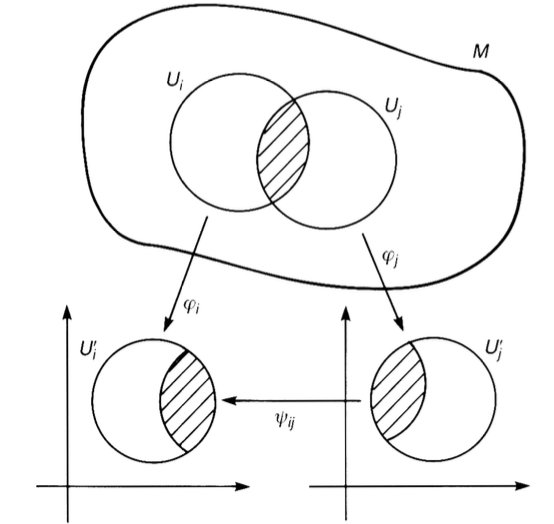
\includegraphics[width=0.5\textwidth]{Images/homeomorphism.png}
	\caption{$\phi_i$ is a homeomorphism from $U_i$ onto an open subset $U'_i$ of $\R^n$.}
	\label{fig:homeomorphism}
\end{figure}

Let's begin by refining the definition~\ref{def:manifold-prev} of a \emph{differentiable manifold}, ~\cite{lee:smooth,tu:manifolds}.

\begin{definition}[Differentiable manifold]
	An $n$-dimensional \emph{differentiable manifold} $\M$ is a topological space equipped with a family of pairs $\{ (U_i, \phi_i) \}$, called an \emph{atlas}, where
	\begin{itemize}
		\item Each $U_i$ is an open set in $\M$, and $\cup_i U_i = \M$.
		\item Each $\phi_i$ is a homeomorphism from $U_i$ onto an open subset $U_i'\subseteq \R^n$, as shown in fig.~\ref{fig:homeomorphism}
		\item For any $U_i$ and $U_j$ with $U_i \cap U_j \neq \emptyset$, the map
		      \begin{equation*}
			      \phi_i \circ \phi_j^{-1} \colon \phi_j (U_i \cap U_j) \to \phi_i(U_i \cap U_j),
		      \end{equation*}
		      is infinitely differentiable.
	\end{itemize}
\end{definition}

Each pair $(U_i, \phi_i)$ is called a \emph{chart}, with $U_i$ the \emph{coordinate neighbourhood} and $\phi_i$ the \emph{coordinate map}. Basically, $\phi_i$ assigns $n$ real \emph{coordinates} $\{x_1(p), \dots, x_n(p)\}$ to each point of $U_i$.

A \emph{manifold with boundary} is defined similarly, except each chart maps into the closed half-space $H^n = \{ (x^1, \dots, x^n) \in R^n | x^n \geq 0 \}$, as showed in fig.~\ref{fig:boundary}.

\begin{figure}
	\centering
	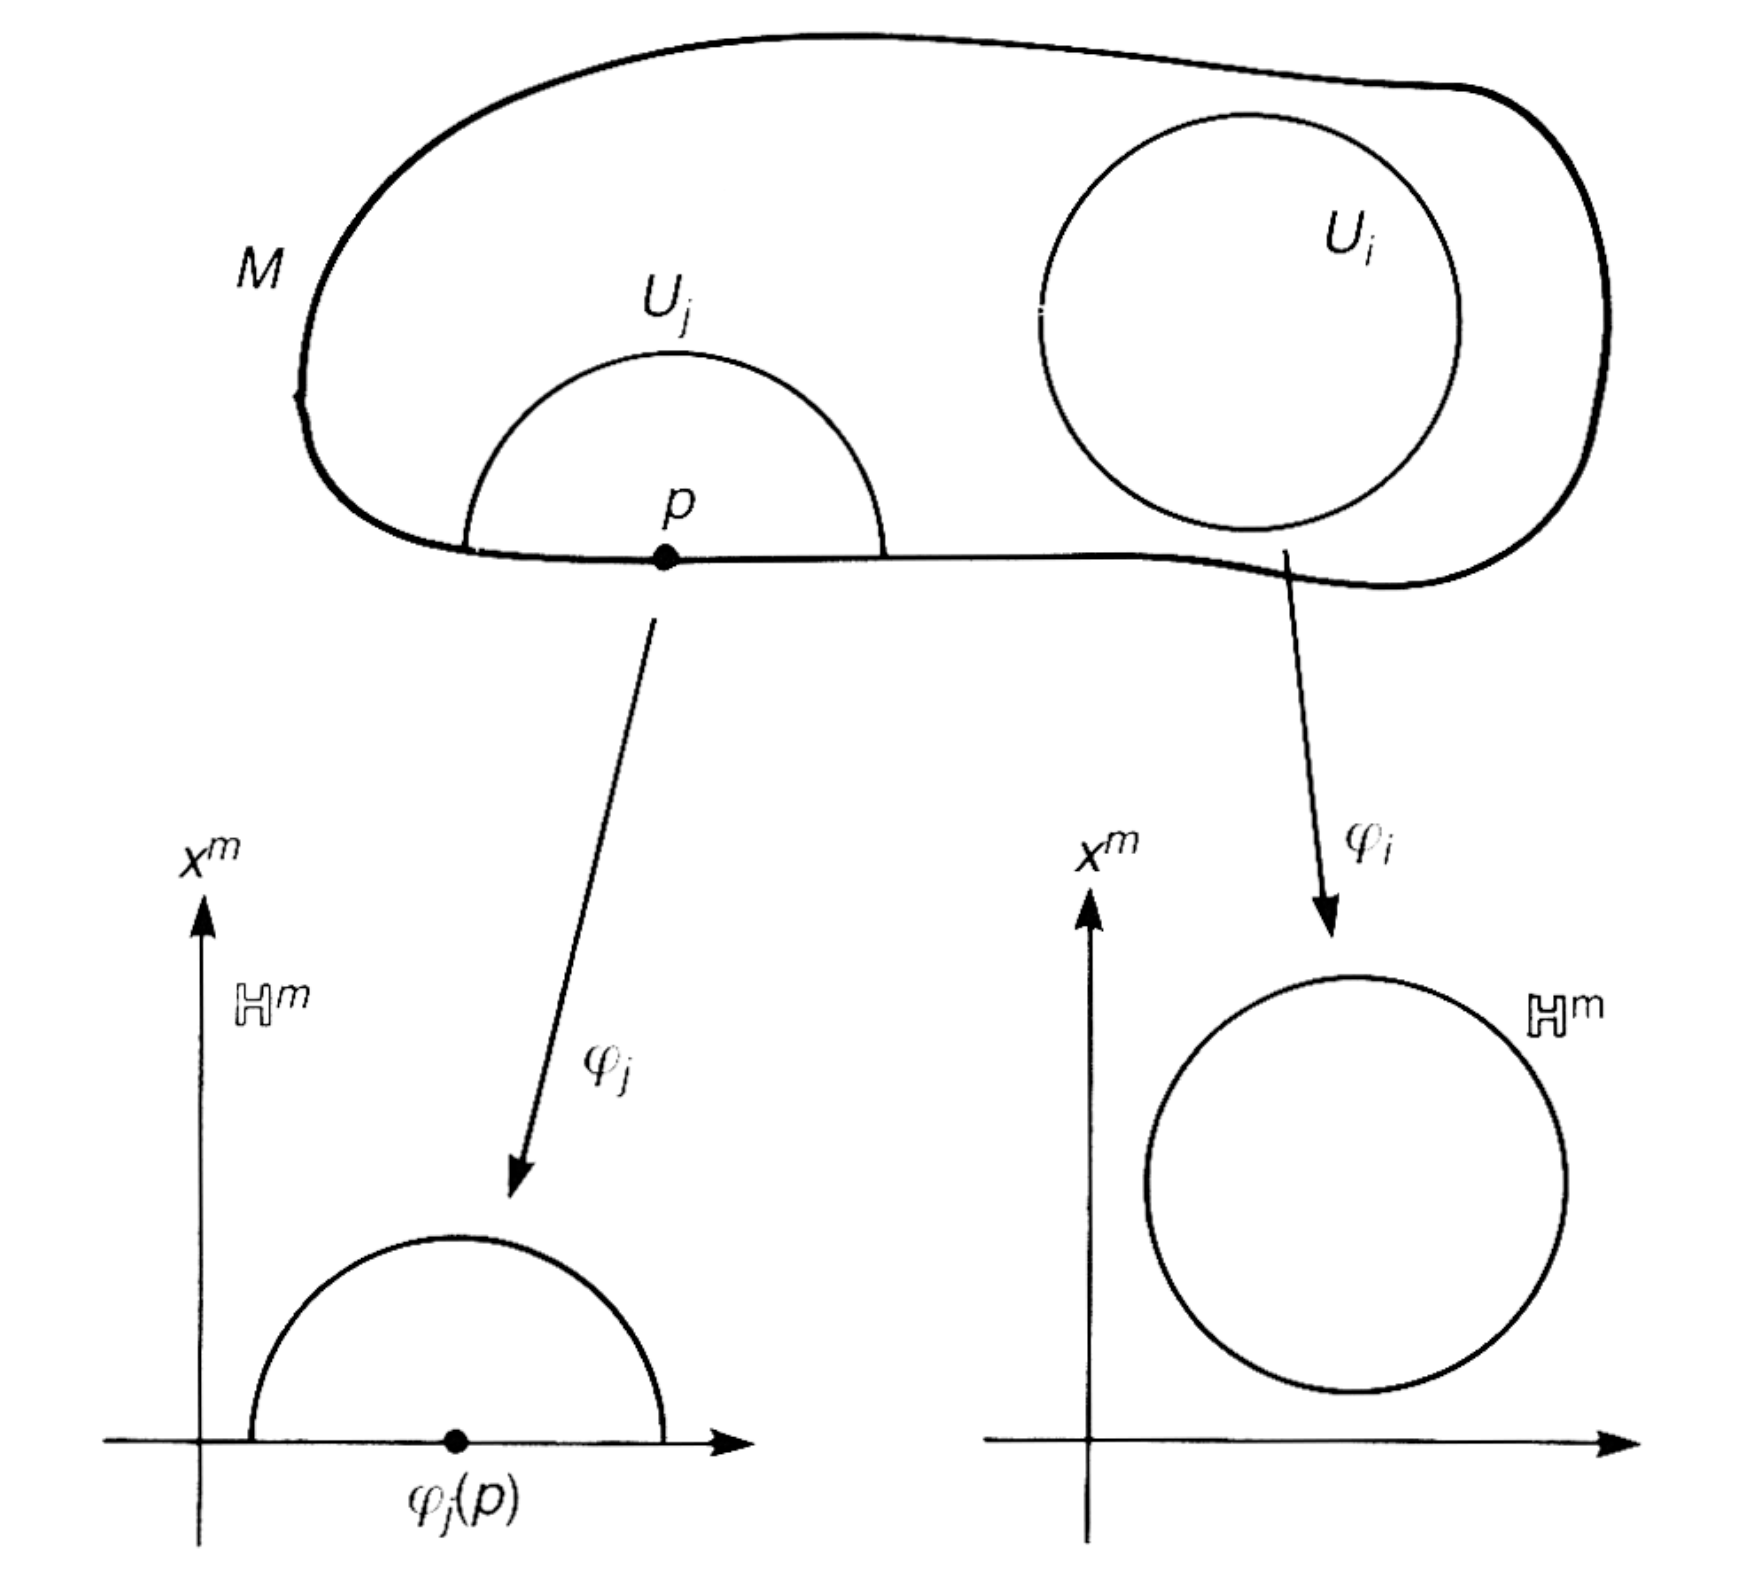
\includegraphics[width=0.5\textwidth]{Images/boundary.png}
	\caption{A manifold $\M$ with boundary. Here, $p \in \de \M$.}
	\label{fig:boundary}
\end{figure}

%***************** DIFFERENTIABLE MAPS ********************
\subsection{Differentiable Maps}
Because each chart maps locally to $\R^n$, we adopt the usual notion of differentiability. Let $\M$ and $\mathcal{N} $ be manifolds of dimension $m$ and $n$, respectively. Consider a map $f: \M \to \mathcal{N}$, as shown in fig.~\ref{fig:map}. Considering the charts $(U, \phi)$ on $\M$ and $(V,\psi)$ on $\mathcal{N}$, the coordinate representation of $f$ is
\begin{equation}
	\phi \circ f \circ \phi^{-1}: \R^m \to \R^n .
\end{equation}

Relaxing the notation, we may write $\phi(p) = \{x^\mu\}$ and $\psi(f(p)) = \{y^\alpha\}$, so that $f$ is \emph{differentiable} at $p \in \M$ if $y^\alpha = f^\alpha(x^\mu)$ is.

\begin{figure}
	\centering
	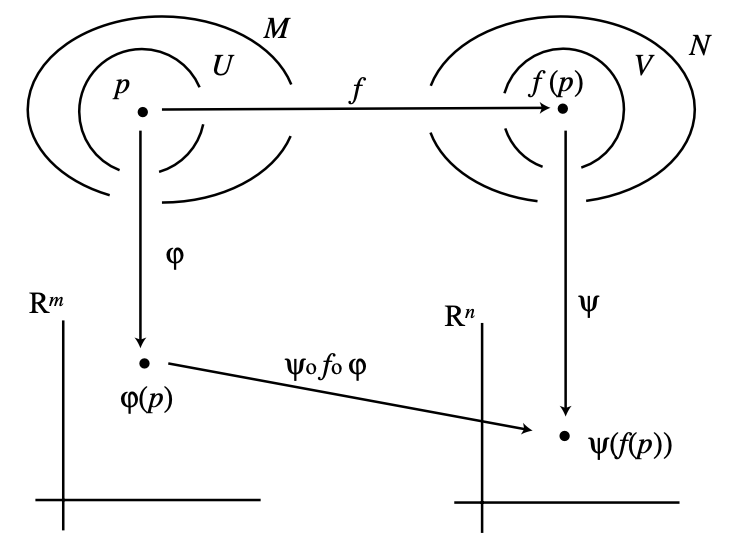
\includegraphics[width=0.5\textwidth]{Images/map.png}
	\caption{A map $f \colon \M \to \mathcal{N}$ has coordinates representation $\psi \circ f \circ \phi^{-1} \colon \R^m \to \R^n$.}
	\label{fig:map}
\end{figure}

Three special classes of differentiable maps are especially relevant.

\begin{definition}[Diffeomorphism]
	Let $f \colon \M \to \mathcal{N}$ be a homeomorphism and $\psi$ and $\phi$ the same coordinate functions as before. Then, if $\psi \circ f \circ \phi^{-1}$ is invertible and both $y \equiv \psi \circ f \circ \phi^{-1}(x)$ and $x \equiv \phi \circ f^{-1} \circ \psi^{-1}(y)$ are $C^\infty$, $f$ is called a \emph{diffeomorphism} and $\M$ is said to be \emph{diffeomorphic} to $\mathcal{N}$, $\M \equiv \mathcal{N}$.
\end{definition}

\begin{definition}[Curve]
	An \emph{open curve} in an $n$-dimensional manifold $\M$ is a map $c \colon (a,b) \to \M$, where $(a,b)$ is an open interval such that $a<0<b$. A \emph{closed curve} is a map $c \colon S^1 \to \M$. On a chart $(U,\phi)$, a curve $c(t)$ ha the coordinate representation $x=\phi \circ c \colon \R \to \R^n$. See fig.~\ref{fig:curve}
\end{definition}

\begin{definition}[Function]
	A \emph{function} $f$ on $\M$ is a smooth map from $\M$ to $\R$. On a chart $(U,\phi)$, the coordinate representation of $f$ is given by $f \circ \phi^{-1} \colon \R^n \to \R$, which is a real-valued function of $n$ variables. The set of functions is denoted by $\mathfrak{F}(\M)$. See fig.~\ref{fig:function}
\end{definition}

\begin{figure}
	\centering
	\begin{subfigure}[b]{0.38\textwidth}
		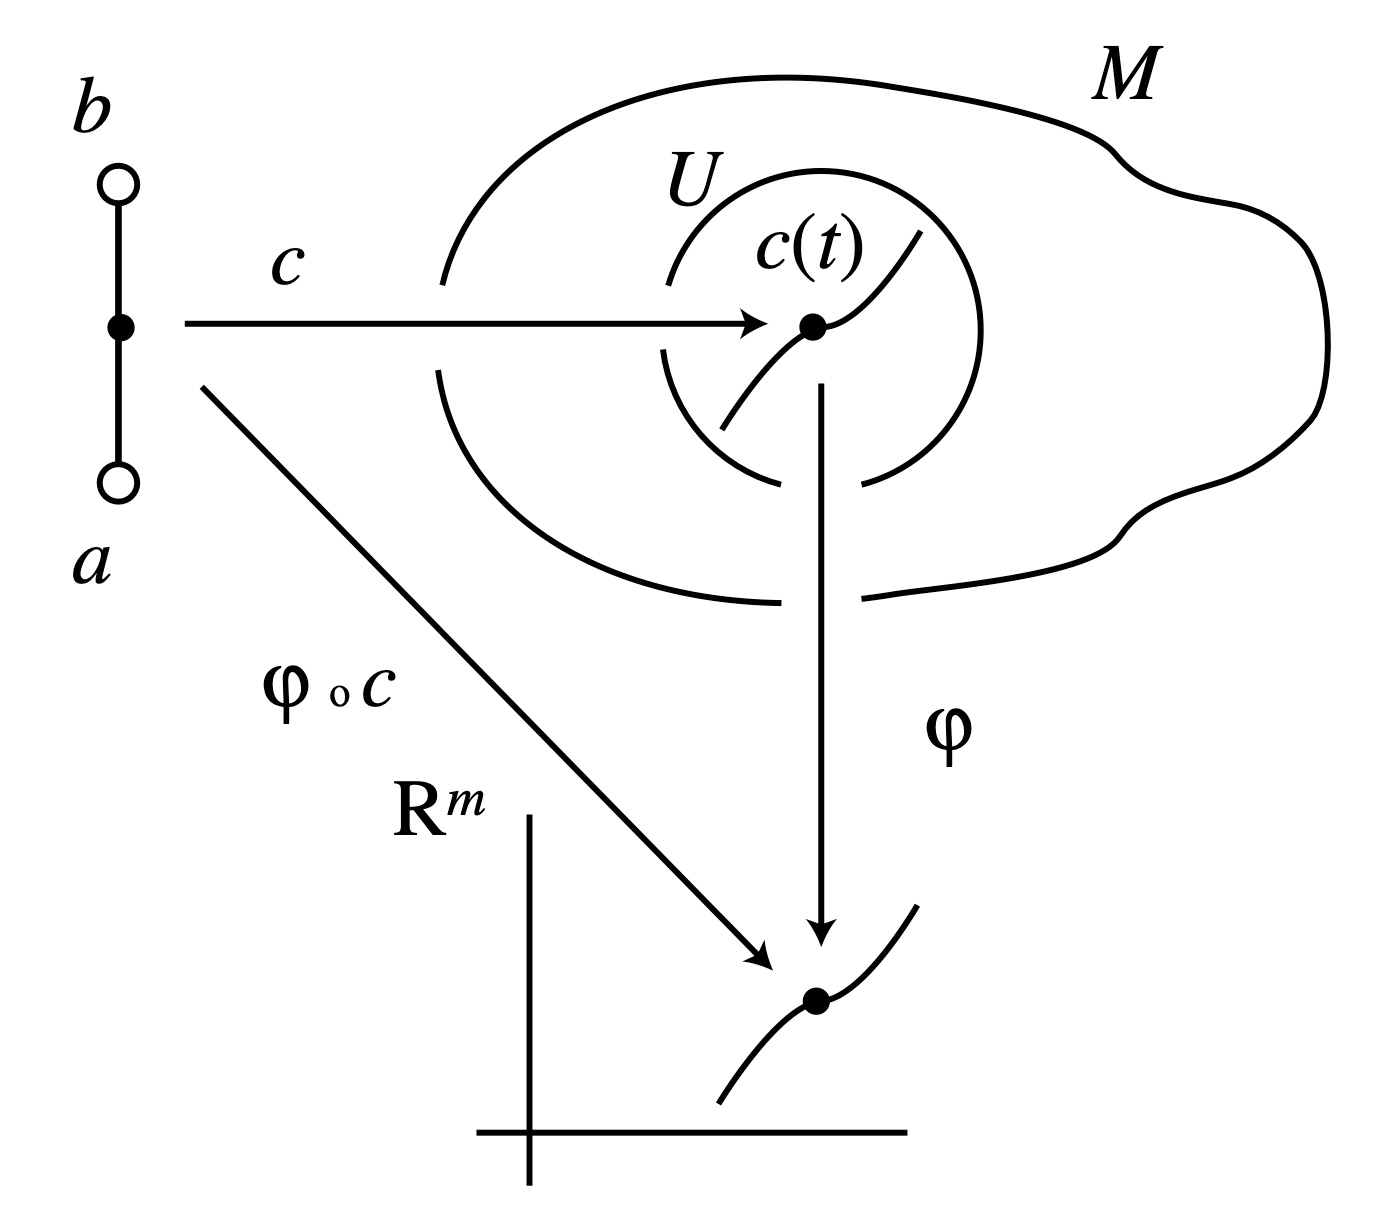
\includegraphics[width=\textwidth]{Images/curve}
		\caption{A curve $c$ in $\M$ and its coordinate representation $\psi \circ c$.}
		\label{fig:curve}
	\end{subfigure}
	\hfill
	\begin{subfigure}[b]{0.42\textwidth}
		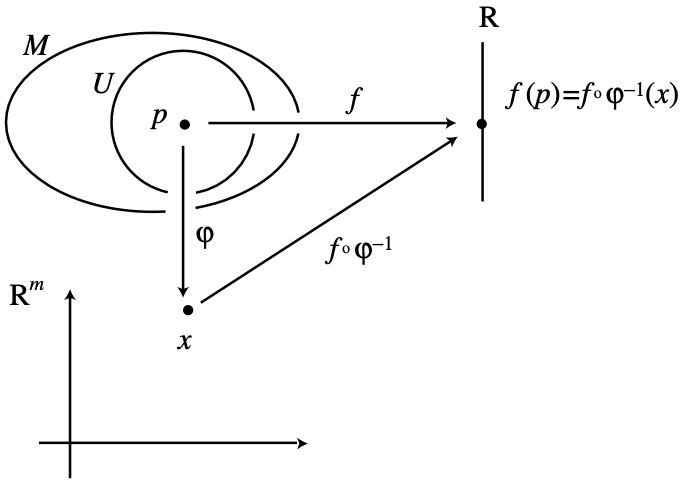
\includegraphics[width=\textwidth]{Images/function.png}
		\caption{A function $f\colon \M \to \R$ and its coordinate representation $f \circ \phi^{-1}$.}
		\label{fig:function}
	\end{subfigure}
	\caption{Curves and functions on a manifold.}
\end{figure}

%***************** VECTORS ********************
\subsection{Vectors}
A useful way to define a \emph{vector} on a manifold is through directional derivatives of functions along curves. Let $c\colon (a,b) \to \M$ be a curve with $c(0)=p$, and let $f \colon \M \to \R$ be any smooth function, as showed in fig.~\ref{fig:vector}. The \emph{tangent vector} at $p$ is the directional derivative of $f(c(t))$ along the curve $c(t)$ at $t=0$, that is,
\begin{equation}
	X[f] \coloneq \left. \frac{\ud f (c(t))}{\ud t}\right|_{t=0} = \left. \frac{\partial f}{\partial x^\mu} \frac{\ud x^\mu(c(t))}{\ud t} \right|_{t=0} = X^\mu \left(\frac{\de f}{\de x^\mu}\right),
\end{equation}
where we defined
\begin{equation}\label{eq:def-vectors}
	X = X^\mu \left(\frac{\de}{\de x^\mu}\right), \quad X^\mu = \left. \frac{\ud x^\mu(c(t))}{\ud t} \right|_{t=0} .
\end{equation}

\begin{figure}
	\centering
	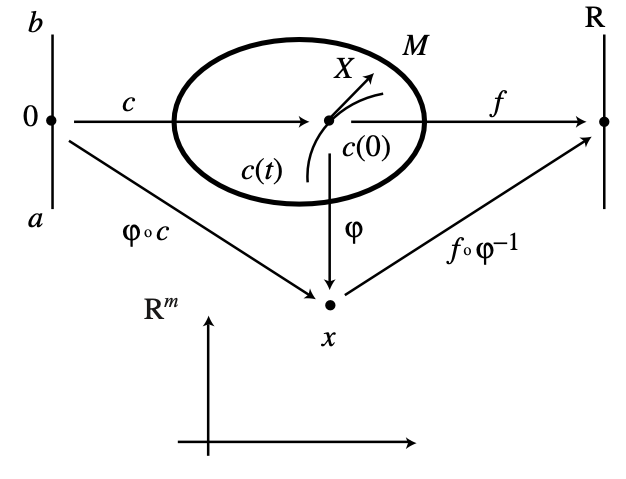
\includegraphics[width=0.5\textwidth]{Images/vector.png}
	\caption{A curve $c$ and a function $f$ define a tangent vector along the curve in terms of directional derivatives.}
	\label{fig:vector}
\end{figure}

Two curves $c_1(t)$ and $c_2(t)$ define the \emph{same} tangent vector at $p$ if
\begin{equation}
	c_1(0)= c_2(0)=p
\end{equation}
and
\begin{equation}
	\left. \frac{\ud x^\mu(c_1(t))}{\ud t} \right|_{t=0} = \left. \frac{\ud x^\mu(c_2(t))}{\ud t} \right|_{t=0} .
\end{equation}

The above relation defines an \emph{equivalence class}, and a vector $X$ at $p\in\M$ is an equivalence class of curves, that is,

\begin{equation}
	[c(t)] = \left\{ \tilde{c}(t) \; \Big| \; \tilde{c}(0) = c(0) \; \textit{and} \; \left. \frac{\ud x^\mu (\tilde{c}(t))}{\ud t}\right|_{t=0} = \left. \frac{\ud x^\mu (c(t))}{\ud t}\right|_{t=0} \right\} .
\end{equation}

The space of all such vectors at $p$ is the \emph{tangent space} $T_p \M$. A basis for $T_p \M$ is given by
\begin{equation}
	\left\{ e_\mu = \frac{\de}{\de x^\mu} \right\}   , \quad \mu = 1, \dots, n,
\end{equation}
making $\dim T_p \M = \dim \M = n$. Further, for each $V \in T_p \M$, we can expand it as $V = V^\mu e_\mu = V^\mu \de_\mu$, and we call $V^\mu$ the components of $V$ with respect to the basis.

%***************** ONE-FORMS ********************
\subsection{One-Forms}
Since each $T_p \M$ is a vector space, its \emph{dual} space $T^*_p \M$, called the \emph{cotangent space}, consists of linear functionals on $T_p \M$. An element 
\begin{equation}
    T^*_p \M \ni \omega \colon T_p \M \to \R
\end{equation}
is called \emph{one-form} at $p$. The simplest example is the \emph{differential} $\ud f$ of a function $f \in \F(\M)$. Its action on a vector $V \in T_p \M$ is given by
\begin{equation}
	\scalar{\ud f}{V} \equiv V[f] = V^\mu \frac{\de f}{\de x^\mu} \in \R.
\end{equation}

In coordinates $x = \phi(p)$, it can be expanded as
\begin{equation}
	\ud f = \frac{\de f}{\de x^\mu} \ud x^\mu,
\end{equation}
which clearly shows that $\{ \ud x^\mu \}$ is a basis of $T^*_p \M$, dual to $\{ \de_\mu \}$, since
\begin{equation}
	\scalar{\ud x^\mu}{\de_\mu} = \frac{\de x^\nu}{\de x^\mu} = \delta^\nu_\mu .
\end{equation}

For a generic one-form $\omega \in T^*_p \M$ and a generic vector $V \in T_p \M$, the \emph{inner product}
\begin{equation}
    \scalar{.}{.}\colon T^*_p \M \times T_p \M \to \R
\end{equation}
is defined by
\begin{equation}\label{eq:def-inner-product-vector-one-form}
	\scalar{\omega}{V} = \omega_\mu V^\mu \scalar{\ud x^\mu}{\de_\nu} = \omega_\mu V^\nu \delta^\mu_\nu = \omega_\mu V^\mu.
\end{equation}

%***************** TENSORS AND TENSOR FIELDS ********************
\subsection{Tensors and Tensor Fields}
In multilinear algebra, a \emph{tensor} of type $(q,r)$ at $p \in \M$ is a multilinear map 
\begin{equation}
	T^{(q,r)} \colon
	\underbrace{T^*_p \M \otimes \dots \otimes T^*_p \M}_\text{$q$ times}
	\otimes
	\underbrace{T_p \M \otimes \dots \otimes T_p \M}_\text{$r$ times} \longrightarrow \R.
\end{equation}

In coordinates, picking dual basis, such a tensor can be expanded as
\begin{equation}
	T^{(q,r)} = \tensor{T}{^{\mu_1}^\dots^{\mu_q}_{\nu_1}_\dots_{\nu_r}} \frac{\de}{\de x^{\mu_1}} \dots \frac{\de}{\de x^{\mu_q}} \ud x^{\nu_1} \dots \ud x^{\nu_r}.
\end{equation}

The set of type $(q,r)$ tensors at $p \in \M$ is denoted by $\Tau^q_{r;p}(\M)$. A vector is a $(1,0)$ tensor, while a one-form is a $(0,1)$ tensor.

In order to probe a manifold structure, it's necessary to have fields defined in it, which are smoothly structures defined for each point of $\M$. Knowing the tensor structure at a point, it's easy to generalize it to the entire manifold.

In particular, for a $(1,0)$ tensor, a \emph{vector field} is a vector assigned smoothly to each point of $\M$. In other words, $V$ is a vector field if $V[f] \in \F(\M)$, for any $f \in \F(\M)$. Hence, each component of a vector field is itself a smooth function from $\M$ to $\R$. We denote the set of vector fields with $\X(\M)$. Then, a vector $X \in \X(\M)$ computed at a point $p \in \M$ is a vector at $T_p \M$, meaning $X|_p \in T_p \M$.

Similarly, a \emph{tensor field} of type $(q,r)$ is a smooth assignment of an element of $\Tau^q_{r;p}(\M)$ at each point $p \in \M$. The set of tensor fields of type $(q,r)$ on $\M$ is denoted by $\Tau^q_r(\M)$.

%***************** FLOW BY VECTOR FIELD ********************
\subsection{Flow generated by a vector field}
A smooth vector field on a manifold naturally gives rise to a flow, a continuous mapping that describes how points move along the trajectories defined by the field.

Specifically, if $X$ is a vector field on $\M$, its associated flow is given by the map
\begin{equation}
    \sigma \colon \R \times \M \to \M,
\end{equation}
such that for each point $x$ in $\M$, the curve defined by $t \mapsto \sigma(t, x)$ is an integral curve of $X$. In other words, at each parameter value $t$ the tangent vector to the curve coincides with the value of $X$ at the point $\sigma(t,x)$.

In local coordinates, if we write $X$ in the form
\begin{equation}
    X = X^\mu \de_\mu,
\end{equation}
then the integral curve passing through an initial point $x_0$ satisfies the system of ordinary differential equations
\begin{equation}\label{eq:ode-flow-coordinates}
	\frac{\ud}{\ud t} \sigma^\mu (t,x_0) = X^\mu (\sigma(t,x_0)),
\end{equation}
with the initial condition
\begin{equation}\label{eq:ode-flow-initial-condition}
	\sigma^\mu(0,x_0) = x^\mu_0.
\end{equation}

A key property of the flow is its group-like behaviour. Indeed, for any two real numbers $t$ and $s$ and for any $x\in\M$, we have
\begin{equation}\label{eq:property-flow}
	\sigma(t, \sigma^\mu(s,x)) = \sigma(t+s,x),
\end{equation}

This property states that flowing first for a parameter $s$ and then for an additional parameter $t$ is equivalent to flowing continuously for a parameter $t + s$. It also implies that each mapping $\sigma(t,\,\cdot)$ is invertible with inverse $\sigma(-t,\,\cdot)$.

Applying the existence and uniqueness theorems for ordinary differential equations, one can prove the following theorem.

\begin{theorem}[Fundamental Existence Theorem for Flows]
	For any point $x \in \M$, there exists a unique differentiable map $\sigma \colon \R \times \M \to \M$, satisfying
	\begin{itemize}
		\item $\sigma(0,x) = x$;
		\item $t \mapsto \sigma(t,x)$ is a solution of~\eqref{eq:ode-flow-coordinates} and~\eqref{eq:ode-flow-initial-condition};
		\item $\sigma(t,\sigma^\mu(s,x)) = \sigma(t+s,x)$.
	\end{itemize}
\end{theorem}

It is important to note that if the vector field $X$ is complete — that is, if every integral curve can be extended for all time — then the flow is globally defined on $\R$. In contrast, if $X$ is not complete, the flow might only exist around $t = 0$.

Just as flows generated by vector fields encode the dynamics of points on a manifold, the Ricci flow encodes the information about the evolution of a manifold's metric. The correct setting to work in is a Riemannian manifold. 


%***************** RIEMANNIAN MANIFOLDS ********************
\subsection{Riemannian Manifolds}
A Riemannian manifold is a smooth manifold equipped with a Riemannian metric.

\begin{definition}
	Let $\M$ be a differentiable manifold. A \emph{Riemannian metric} $g$ on $\M$ is a type $(0,2)$ tensor field on $\M$ such that, at each point $p \in \M$:
	\begin{itemize}
		\item $g_p (U,V) = g_p (V,U)$,
		\item $g_p(U,V) \geq 0$, where the equality holds only when $U=0$.
	\end{itemize}
	Here, $U,V \in T_p \M$ and $g_p = g|_p$. Basically, $g_p$ is a symmetric positive-definite bilinear form.
\end{definition}

Recall the previous definition of inner product~\eqref{eq:def-inner-product-vector-one-form} between vectors and dual forms. For $V \in T_p \M$ and $\omega \in T^*_p \M$, the inner product is given by $\scalar{.}{.} \colon T^*_p \M \times T_p \M \to \R$. If there exists a metric tensor $g$, then, we can use it to define the inner product between two vectors $U,V \in T_p \M$, specifically by $g_p(U,V)$. Since $g_p \colon T_p \M \otimes T_p \M \to \R$, we may define a linear map $g_p(U,.) \colon T_p \M \to \R$ by $V \mapsto g_p(U,V)$. Then, it's straightforward that $g_p(U,.) \in T^*_p \M$ is a one-form. Thus, the metric $g_p$ gives rise to an isomorphism between $T_p \M$ and $T^*_p \M$.

Choosing a chart $(\phi,U)$, with coordinates $\{ x^\mu \}$, we can express the metric tensor in local coordinates as
\begin{equation}
	g_p = g_{\mu\nu}(p) \ud x^\mu \otimes \ud x^\nu, \quad g_{\mu\nu}(p) = g_p (\de_\mu, \de_\nu) = g_{\nu\mu}(p), \quad p \in \M.
\end{equation}

It is usual convention to omit the point $p$, denote the inverse metric as $g^{\mu\nu}$, and the determinant as $\det(g_{\mu\nu}) \coloneq g$ and $\det(g^{\mu\nu}) \coloneq g^{-1}$. Thus, the isomorphism between $T_p \M$ and $T^*_p \M$ can be expressed as
\begin{equation}
	\omega_\mu = g_{\mu\nu} U^\nu, \quad U^\mu = g^{\mu\nu} \omega_\nu .
\end{equation}

%***************** COVARIANT DERIVATIVE ********************
\subsection{Covariant Derivatives}
In a curved manifold, the standard notion of differentiation does not preserve the tensorial character of geometric objects. To overcome this difficulty, we introduce the concept of the \emph{covariant derivative}. It extends the idea of directional derivatives to curved spaces, and allows us to define the concept of parallelism on a manifold.

To define this, we first introduce the concept of an \emph{affine connection}.
\begin{definition}
    An \emph{affine connection} $\nabla$ is a map $\nabla \colon \X(\M) \times \X(\M) \to \X(\M)$, or $(X,Y) \mapsto \nabla_X Y$ which satisfies the following conditions
    \begin{subequations}
        \begin{align}
            \nabla_X (Y + Z) &= \nabla_X Y + \nabla_X Z \\
            \nabla_{(X+Y)} Z &= \nabla_X Z + \nabla_Y Z \\
            \nabla_{(fX)} Y &= f \nabla_X Y \\
            \nabla_X (fY) &= X[f] Y + f \nabla_X Y,
        \end{align}
    \end{subequations}
    where $f \in \F(\M)$ and $X,Y,Z \in \X(\M)$.
\end{definition}

Take a chart $(U, \phi)$ with the coordinate $x = \phi(p)$ on $\M$, and define the functions $\Gamma^\lambda_{\nu\mu}$ called \emph{Christoffel symbols}, by
\begin{equation}
    \nabla_\nu e_\mu \equiv \nabla_{e_\nu} e_\mu = e_\lambda \Gamma^\lambda_{\nu\mu},
\end{equation}
where $\{e_\mu\} = \{\de_\mu\}$ is the coordinate basis in $T_p \M$.

Once the action of $\nabla$ on the basis vectors is defined, we can compute its action on any vectors, in particular
\begin{equation}\label{eq:def-cov-der}
    \nabla_V W = V^\mu \left( \frac{\de W^\lambda}{\de x^\mu} + W^\nu \Gamma^\lambda_{\mu\nu} \right) e_\lambda .
\end{equation}

In particular, $\nabla$ maps two vectors $V$ and $W$ to a new vector given by the right-hand side of eq.~\eqref{eq:def-cov-der}, whose $\lambda$th component is $V^\mu \nabla_\mu W^\lambda$, where
\begin{equation}
    \nabla_\mu W^\lambda \equiv \frac{\de W^\lambda}{\de x^\mu} + \Gamma^\lambda_{\mu\nu} W^\nu
\end{equation}

Beyond vector fields, the concept of the covariant derivative extends naturally to tensor fields of any rank. For a general tensor field $T$ of type $(q, r)$, the covariant derivative $\nabla T$ is defined to behave as a tensor of type $(q, r+1)$ and to satisfy the appropriate product rule with respect to the tensor contractions and tensor products.

For Riemannian manifolds endowed with a metric tensor $g$, the affine connection can be chosen to be \emph{compatible} with the metric, meaning that
\begin{equation}
    \nabla_X g = 0, \quad \forall X \in \X(\M).
\end{equation}
Intuitively, this means that angles between vectors are conserved while parallelly transporting them along each other.

%***************** CURVATURE ********************
\subsection{Curvature and Ricci Tensor}

Curvature provides a quantitative measure of how a manifold deviates from being flat. Since $\Gamma$ is not a tensor, it can't have an intrinsic geometric meaning as a measure of the curvature. To serve this purpose, one introduces the \emph{tortion tensor} $T \colon \X(\M) \otimes \X(\M) \to \X(\M) $ and the \emph{Riemann tensor} $R \colon \X(\M) \otimes \X(\M) \otimes \X(\M) \to \X(\M) $. They're defined by
\begin{align}
    T(X, Y) &\equiv \nabla_X Y - \nabla_Y X - [X,Y], \\
    R(X,Y,Z) &\equiv \nabla_X \nabla_Y Z - \nabla_Y \nabla_X Z - \nabla_{[X,Y]} Z. \label{eq:def-riemann}
\end{align}

For simplicity, we consider torsionless connections, for which the Christoffel symbols are symmetric, meaning that
\begin{equation}
    \Gamma^\lambda_{\nu\mu} = \Gamma^\lambda_{\mu\nu} .
\end{equation}

Further, for a metric compatible connection, one can derive the following expression
\begin{equation}
    \Gamma^\lambda_{\mu\nu} = \frac{1}{2} g^{\lambda\rho} \left( \de_\nu g_{\mu\rho} + \de_\mu g_{\nu\rho} - \de_\rho g_{\mu\nu} \right),
\end{equation}
and the Riemann tensor has components
\begin{equation}
    R_{\mu\nu\rho\sigma} = \frac{1}{2} \left( \de_{\nu\rho} g_{\mu\sigma} - \de_{\nu\sigma} g_{\mu\rho} + \de_{\mu\sigma} g_{\nu\rho} - \de_{\mu\rho} g_{\nu\sigma} \right) .
\end{equation}

Using the general definition~\eqref{eq:def-riemann}, one can prove the following identities
\begin{subequations}
\begin{gather}
    R_{\mu\nu\rho\sigma} = - R_{\nu\mu\rho\sigma} = - R_{\mu\nu\sigma\rho} \\
    R_{\mu\nu\rho\sigma} = R_{\rho\sigma\mu\nu} \\
    R^\mu_{\nu\rho\sigma} + R^\mu_{\sigma\nu\rho} + R^\mu_{\rho\sigma\nu} = 0
\end{gather}
\end{subequations}

The symmetries allow us to define the symmetric tensor $R_{\mu\nu} = R^\lambda_{\mu\lambda\nu}$, called \emph{Ricci tensor}, and the \emph{Ricci scalar} $R = R^\mu_\mu$.
%**************** NON-LINEAR SIGMA MODELS AND STRINGS ******************
\section{Non-Linear Sigma Models and String Theory}
The standard starting point of string theory is \emph{Polyakov action}, which describes a bosonic classical, one-dimensional, string, which describes a two-dimensional worldsheet $\Sigma$ on a $26$-dimensional spacetime described by the spacetime coordinates $X^\mu(\xi)$, $\mu = 0, \dots 25$, where $\xi^a = (\tau, \sigma)$, $a = 1,2$, are the intrinsic coordinates on $\Sigma$. The metric on spacetime is denoted by $g_{\mu\nu}$, while the metric on the worldsheet is $\gamma_{ab}$. For a flat spacetime, with Minkowski metric $g_{\mu\nu} \equiv \eta_{\mu\nu} = \textup{diag}(-1,+1,+1,+1)$, the action reads
\begin{equation}\label{eq:polyakov}
    S_P [X^\mu(\xi), \gamma_{ab}(\xi)] = -\frac{T}{2} \int_\Sigma \ud \tau \ud \sigma \sqrt{-\det(\gamma)} \gamma^{ab} \de_a X_\mu (\xi) \de_b X^\mu (\xi),
\end{equation}
where $T$ is a characteristic parameter of the string, related to the string length $l$.

The symmetries of this action allow us to consider a flat worldsheet metrix, $\gamma_{ab} = \eta_{ab}$, considering the so-called \emph{unit gauge}. Then, reintroducing explicitly the metric $g_{\mu\nu}$, even if it's flat in this case, we obtain
\begin{equation}\label{eq:polyakov-metric}
    S_P = - T \int_\Sigma \ud^2 \xi g_{\mu\nu}(X) \de_a X^\mu \de^a X^\nu.
\end{equation}

Basically, it represents a 2-dimensional field theory on the worldsheet, where the coordinates $X^\mu$ are 26 dynamical fields in there. This allows us to quantize the theory with the usual quantization prescription, based on the substitution of the classical Poisson brackets defined on a symplectic manifold with the commutators of operators acting on a Hilbert space.

After quantization, one notice that, for a closed string, defined by the periodicity condition $X^\mu(\tau,\sigma) = X^\mu (\tau, \sigma + l)$, the particle spectrum contains a \emph{graviton} $\gamma_{\mu\nu}$, which resembles a gravitational wave at low energies, a scalar field $\phi$ called \emph{dilaton} and an antisymmetric two-tensor $b_{\mu\nu}$ called \emph{Kalb-Ramond tensor}.

Therefore, due to the presence of the graviton, one could wonder what happens for a non-flat spacetime. Then, after redefining the coordinates as a constant $X^\mu_0$ plus some other arbitrary fields $Y^\mu$, i.e.,
\begin{equation}
    X^\mu (\xi) = X^\mu_0 (\xi) + \sqrt{\alpha'} Y^\mu (\xi),
\end{equation}
we can expand the term in the Lagrangian as
\begin{equation}\label{eq:expansion-coordinates}
\begin{split}
    &g_{\mu\nu}(X) \de_a X^\mu \de^a X^\nu \\
    &= \alpha' \left[ g_{\mu\nu}(X_0) + \sqrt{\alpha'} g_{\mu\nu,\rho}(X_0)Y^\rho(\xi) + \frac{\alpha'}{2} g_{\mu\nu,\rho\sigma}(X_0)Y^\rho(\xi Y^\sigma(\xi)) + \dots \right] \de_a Y^\mu \de^a Y^\nu ,
\end{split}
\end{equation}
where $g_{\mu\nu,\rho} \equiv \de_\rho g_{\mu\nu}$. 

We obtained an expansion in $\alpha'$, where each term is an interaction term for the fields $Y^\mu$, with couplings given by the derivatives of the metric. However, a crucial symmetry of the Polyakov action~\eqref{eq:polyakov} is the invariance under \emph{conformal transformations}. Those are diffeomorphisms on a Riemannian Manifold which preserve the metric up to rescaling, i.e.,
\begin{equation}\label{eq:conformal-transformation}
    g(x) \to \tilde{g}(\tilde{x}) = e^{2\omega(\tilde{x})} g(\tilde{x}).
\end{equation}

Without going into the details, the presence of this symmetry is considered as a consistency condition for the theory, as it allows for a perturbative interpretation of the interactions. In addition, the above interacting quantum field theory must undergo renormalization, in order to cure the divergences. 

However, after renormalization, the conformal symmetry may be anomalous\footnote{An anomaly is a classical symmetry which is not preserved at the quantum level. In particular, it is due to a non-invariance of the measure of the path integral.}. Indeed, a particular example of conformal transformation~\eqref{eq:conformal-transformation} is provided by scale-invariance. That is to say, the theory can't depend on a scale to be conformal invariant. But, as the methods of \emph{renormalization group} teach us, after renormalization the couplings run with the energy scale $M$ of the system, dependence which is encapsulated into the \emph{$\beta$-function}
\begin{equation}
    \beta(g_{\mu\nu}) = M \frac{\de}{\de M} g_{\mu\nu}.
\end{equation}

As a consequence, for a quantum string theory to make sense, it must be conformal invariance, so the $\beta$-function associated to the metric, in the action~\eqref{eq:polyakov-metric} with the expansion~\eqref{eq:expansion-coordinates}, must vanish
\begin{equation}
    \beta(g_{\mu\nu}) \overset{!}{=} 0.
\end{equation} 

A similar argument can be pursued for the other two particles in the closed string spectrum, i.e., the dilaton $\phi$ and the Kalb-Ramond form $b_{\mu\nu}$. The corresponding action will be
\begin{equation}
    S_\sigma = -\frac{T}{2} \int_\Sigma \ud^2 \xi \sqrt{-\det(\gamma)}\left[ \left( \gamma^{ab} g_{\mu\nu}(X) + i \epsilon^{ab} b_{\mu\nu}(X) \right) \de_a X^\mu \de_b ^\nu + \alpha' \mathcal{R} \phi(X) \right],
\end{equation}
where $\epsilon^{ab}$ is the $2$d Levi-Civita symbol, while $\mathcal{R} = \mathcal{R}(\gamma)$ is the Ricci scalar on the worldsheet.

Defining the Field Strength $H_{\mu\nu\rho} = \de_\mu b_{\nu\rho} + \de_\nu b_{\rho\mu} + \de_\rho b_{\mu\nu}$, the vanishing of the beta functions reads
\begin{subequations}\label{eq:beta-functions}
\begin{align}
    \beta(g_{\mu\nu}) &= \alpha' \left( R_{\mu\nu} - \frac{1}{4} H_{\mu\lambda\rho} H^{\mu\lambda\rho} + 2 \cov_\mu \cov_\nu \phi \right) + O(\alpha'^2)\overset{!}{=} 0,\\
    \beta(b_{\mu\nu}) &= \alpha' \left( \frac{1}{2} \cov^\rho H_{\rho\mu\nu} + \cov^\rho \phi H_{\rho\mu\nu} \right) + O(\alpha'^2)\overset{!}{=} 0, \\
    \beta(\phi) &= \alpha' \left( \frac{1}{2} \cov_\mu \phi \cov^\mu \phi - \frac{1}{2} \cov^2 \phi - \frac{1}{24} H_{\mu\nu\rho} H^{\mu\nu\rho} \right) + O(\alpha'^2)\overset{!}{=} 0.
\end{align}
\end{subequations}

The above equations are constraints for the spacetime fields $(g,b,\phi)$, imposed to preserve conformal invariance of the quantum string. However, since those fields should be dynamical on spacetime, those must also be their equations of motion. This leads to the following \emph{low-energy effective action}, which has~\eqref{eq:beta-functions} as equations of motion
\begin{equation}
    S_{26} = \frac{1}{k^2_0} \int \ud^{26}x \sqrt{\det(g)} e^{-2\phi} \left( \mathcal{R}(g) - \frac{1}{12} H_{\mu\nu\rho} H^{\mu\nu\rho} + 4 \cov_\mu \phi \cov^\mu \phi \right).
\end{equation}

To set this problem to a more general ground, and understand how this model is related to Ricci-Flow, let's define more accurately what a $\sigma$-model is in field theory.
%**************** RICCI FLOW FOR TOPOLOGY ******************
\section{Ricci Flow to Tackle Topological Problems}

\chapter{Ricci Flow and Oliver-Ricci Curvature}
%**************** INTRODUCTION TO OLLIVIER RICCI CHAPTER ******************
Initially introduced by Richard S.~Hamilton in the early 1980s, Ricci Flow arose historically as a powerful method in differential geometry. At its heart, it seeks to ``smooth out'' geometric irregularities of manifolds by evolving the underlying Riemannian metric through a partial differential equation (PDE) reminiscent of the classical heat equation. We recall that a manifold is a topological space locally resembling Euclidean space, and a \emph{Riemannian manifold} is such a space equipped with an inner product on each tangent space, making it possible to measure angles, distances, and curvature. 

Curvature, in particular, is fundamental to geometry: it describes how space bends or deviates from flatness. On a two-dimensional surface embedded in three-dimensional space, for example, curvature can be visualized by examining the deviation of geodesics (the generalization of ``straight lines'' in curved spaces) from parallelism, or by looking at how areas or angles are distorted compared to those in flat Euclidean geometry. The extension to higher dimensions and more abstract manifolds involves careful definitions but retains this key notion of ``spatial bending.'' 



\section{Riemannian Geometry and Curvature Notions}
In classical Riemannian geometry, curvature can be examined from multiple perspectives. One can study the \emph{sectional curvature}, which measures how a two-dimensional plane (spanned by two tangent directions) curves. One can also investigate the \emph{Ricci curvature}, which is obtained by summing or averaging the sectional curvatures over all planes containing a given direction. Ricci curvature has special importance: for instance, it appears in Einstein’s equations of General Relativity, linking geometry to matter and energy distributions in spacetime. 

Concretely, let $(M,g)$ be a Riemannian manifold, where $M$ is a smooth manifold and $g$ is the metric tensor. The Ricci curvature $\mathrm{Ric}$ is derived as a contraction of the Riemann curvature tensor, itself an operator capturing how much nearby geodesics converge or diverge. Positive Ricci curvature typically implies that geodesics tend to converge, reflecting a ``crowded'' or positively curved geometry akin to the sphere. Negative Ricci curvature implies geodesics tend to diverge, mirroring a hyperbolic or “saddle-like” structure. Zero Ricci curvature is the hallmark of Ricci-flat manifolds, with many implications for geometry and topology.

\subsection{Hamilton's Ricci Flow Equation}
Hamilton introduced the Ricci Flow as the PDE:
\[
\frac{\partial g_{ij}}{\partial t} = -2 \, R_{ij},
\]
where $g_{ij}$ are the components of the metric tensor $g$ in local coordinates and $R_{ij}$ are the components of the Ricci curvature tensor. Informally, each infinitesimal piece of the manifold changes in time, guided by curvature. Regions of \emph{high positive} Ricci curvature shrink faster, while regions of \emph{negative} Ricci curvature expand. This leads to a \emph{flow} that tends to smooth out the geometric and topological features of $M$. 

One of the most famous applications of Ricci Flow on manifolds is Grigori Perelman's resolution of the Poincar\'{e} Conjecture and the more general Geometrization Conjecture for three-dimensional manifolds. Perelman’s work introduced the notion of \emph{Ricci Flow with surgery}, a procedure to remove singular regions (places where curvature blows up to infinity) and continue the flow on the remaining parts. In 3D manifolds, these singularities can be visualized as ``neck pinches'' that effectively separate the manifold into topologically simpler pieces. Perelman showed that by performing a series of well-defined surgeries, one could decompose a three-dimensional manifold into model geometric pieces, completing Hamilton’s program toward a proof of the Geometrization Conjecture.

\subsection{From Smooth Settings to Discrete Geometry}
While Ricci Flow is classically defined on smooth manifolds, there has been considerable interest in transferring these ideas to \emph{discrete} or combinatorial settings such as polyhedral surfaces, graphs, and complex networks. The general question is how to define concepts like ``curvature'' when one does not have a smooth manifold or a Riemannian metric in the usual sense. Instead, discrete analogs focus on adjacency, distances along edges, and combinatorial properties that mimic or reflect continuum notions.

For surfaces composed of polygons (triangulations), one can define the curvature at a vertex via angle deficits, a concept dating back to classical differential geometry of polyhedral surfaces. However, for higher-dimensional graphs and networks that are not neatly embedded in any Euclidean space, a more general curvature definition is needed—one that depends mostly on the underlying distances and probability measures rather than an explicit embedding. 
\section{Optimal Transport and Ollivier's Ricci Curvature}
A major breakthrough in defining a curvature notion for general metric spaces (including discrete networks) came via \emph{optimal transport}. Historically, the optimal transport problem, originating in the work of Gaspard Monge in the 18th century, asks how to map one mass distribution into another with minimal transportation cost. Subsequent reformulations by Leonid Kantorovich turned this into a linear optimization problem known as the \emph{Kantorovich relaxation}. 

If $(X, d)$ is a metric space, and we have two probability measures $\mu$ and $\nu$ on $X$, the \emph{Wasserstein distance} (also called the earth mover’s distance) measures how much ``effort'' is needed to move mass from $\mu$ to $\nu$, given the metric $d$. Specifically, one solves an optimization problem that tries to minimize the total cost of moving infinitesimal amounts of mass from one location to another. 

Yann Ollivier harnessed this framework to define a notion of \emph{coarse Ricci curvature} on general metric measure spaces. Ollivier’s definition, now widely called \emph{Ollivier Ricci curvature}, is based on considering small probability balls of radius $\varepsilon$ around points (or sometimes discrete probability measures concentrated on nearest neighbors in a graph) and calculating how much these small balls cost to move one onto the other under optimal transport. If moving these balls requires comparatively more effort than just their pairwise distance would suggest, the edge or connection between them is deemed negatively curved; if it requires less effort, it is positively curved. This emerges from an analog of the well-known statement in Riemannian geometry that Ricci curvature controls how geodesic balls deviate from each other, which can be recast in terms of mass transport.

\chapter{Application to Complex Networks}
To adapt Ollivier's construction to a graph $G = (V,E)$ where $V$ is the set of nodes and $E$ is the set of edges (possibly with weights), one often assigns to each node $x$ a probability measure $m_x$. A typical choice is to concentrate the mass uniformly on $x$’s neighbors, possibly with some parameter $\alpha$ to keep a fraction of the mass at $x$ itself. Let $W(m_x, m_y)$ denote the Wasserstein distance between $m_x$ and $m_y$. The Ollivier Ricci curvature $\kappa(x,y)$ along the edge $(x,y)$ is defined as 
\[
\kappa(x,y) \;=\; 1 \;-\;\frac{W\bigl(m_x, m_y\bigr)}{d(x,y)},
\]
where $d(x,y)$ is the usual shortest-path distance (or a weight-based distance) between $x$ and $y$. Intuitively:
\begin{itemize}
    \item If many of the neighbors of $x$ align well with the neighbors of $y$, then $W(m_x,m_y)$ is relatively small compared to $d(x,y)$, giving a larger curvature.
    \item If the neighbors do not overlap much, $W(m_x,m_y)$ will be comparatively large, implying smaller (or possibly negative) curvature.
\end{itemize}
This lines up with the idea that a highly ``clustered'' or cohesive set of nodes—often indicating an underlying community—acts more like a positively curved region in the manifold analogy, whereas edges bridging distant clusters reflect negative curvature. These insights lead to a method for analyzing and partitioning networks by focusing on edges with specific curvature characteristics.




\section{ARI, Modularity, and Performance}
\label{sec:ricci_flow_networks}

In the study of complex networks, a fundamental task is to identify densely connected groups of nodes, commonly referred to as \emph{communities}. These communities often correspond to meaningful substructures such as friend groups in social networks, functionally related proteins in biological networks, or topics in citation networks. There are numerous algorithms that aim to extract communities---ranging from graph partitioning heuristics and centrality-based edge removal to statistical and probabilistic methods.

The Ricci Flow-based technique for network community detection focuses on the geometric viewpoint: an edge with significantly negative Ricci curvature may signify a \emph{bridge} between distinct communities, whereas edges with positive curvature are typically nestled within cohesive communities. Iteratively adjusting edge weights according to Ollivier Ricci curvature has the effect of “magnifying” bridging edges and “contracting” internal edges, ultimately making a subsequent threshold-based cut reveal the inherent clusters.

Here are the major steps (in broad terms) for using Ricci Flow to detect communities:
\begin{enumerate}
    \item \textbf{Initialization}: Assign an initial weight to each edge $(x,y)$. Often, one starts with uniform weights or with weights based on an existing property such as adjacency or similarity.
    \item \textbf{Probability Measures}: Choose how to define the measure $m_x$ at each node $x$. A popular simple choice is to put uniform weight on all neighbors of $x$, ensuring $\sum_{v \in \text{neighbors}(x)} m_x(v)=1$. Other weighting schemes (e.g., discounting more distant neighbors) can also be used.
    \item \textbf{Curvature Computation}: For each edge $(x,y)$, compute the Ollivier Ricci curvature $\kappa(x,y)$ by solving the discrete optimal transport problem and using 
    \[
    \kappa(x,y) = 1 - \frac{W(m_x, m_y)}{d(x,y)}.
    \]
    \item \textbf{Discrete Ricci Flow Update}: Adjust the edge weight according to
    \[
    w_{xy}^{(i+1)} = w_{xy}^{(i)} \;-\; \eta \,\kappa_{xy}^{(i)} \; d_{xy}^{(i)}.
    \]
    Often, one sets $\eta=1$ and updates all edges simultaneously, then recomputes shortest path distances $d(\cdot,\cdot)$ for the next iteration. The total number of iterations can be chosen based on convergence criteria or practical heuristics.
    \item \textbf{Network Surgery}: After a certain number of iterations, examine the distribution of edge weights. Typically, bridging edges (those connecting separate communities) will have grown in length. Choose a threshold $T$ such that edges with $w_{xy} > T$ are considered “cuts,” removing them from the graph. The connected components that remain are taken as the identified communities.
    \item \textbf{Post-Processing}: If a graph has hierarchical communities, additional steps (e.g., repeating the process within subcomponents) might be performed to further subdivide the clusters.
\end{enumerate}

This pipeline is quite flexible in terms of parameter choices (e.g., the measure definition, the number of flow iterations, the threshold for edge cuts) and can adapt to various network topologies. The next subsections explain how to measure the resulting partition quality, focusing on two widely employed tools: the \emph{Adjusted Rand Index (ARI)} and \emph{Modularity}.

\subsection{Adjusted Rand Index (ARI)}
\label{subsec:ARI_definition}

\subsubsection{General Definition}
The \emph{Adjusted Rand Index (ARI)} is a popular external validation measure to compare a discovered clustering with a known ground-truth partition. Suppose you have a set of $n$ items (in our case, the $n$ nodes of a network). Let $C = \{C_1, \ldots, C_r\}$ be a partition of these items into $r$ clusters found by some method, and let $G = \{G_1, \ldots, G_s\}$ be the ground-truth (or reference) partition into $s$ clusters. The Rand Index (RI) measures the fraction of item pairs that are \emph{consistently} assigned in both partitions (i.e., either assigned together in both or assigned to different clusters in both). 

Formally, the Rand Index is given by:
\[
\mathrm{RI}(C,G) \;=\; \frac{a + d}{a + b + c + d},
\]
where 
\begin{itemize}
    \item $a$ is the number of pairs of items that are in the same cluster in $C$ \emph{and} in the same cluster in $G$,
    \item $b$ is the number of pairs of items that are in the same cluster in $C$ but in different clusters in $G$,
    \item $c$ is the number of pairs that are in different clusters in $C$ but in the same cluster in $G$,
    \item $d$ is the number of pairs that are in different clusters in $C$ and in different clusters in $G$.
\end{itemize}
Because $a+d$ counts all the agreements (put together or kept apart) and $b+c$ counts the disagreements, $\mathrm{RI}(C,G)$ is between 0 and 1, with 1 meaning a perfect match of the partitions.

However, the Rand Index does not correct for chance agreement. The \emph{Adjusted Rand Index} refines this by subtracting the expected RI of random partitions and rescaling. One can define:
\[
\mathrm{ARI}(C,G) \;=\; \frac{\mathrm{RI}(C,G)\;-\;\mathrm{Expected}[\mathrm{RI}]}{\max(\mathrm{RI})\;-\;\mathrm{Expected}[\mathrm{RI}]},
\]
which yields a value that ranges from 0 (or negative, depending on definition) up to 1. Here, 1 indicates the clustering $C$ exactly matches the ground-truth $G$, whereas an ARI near 0 suggests random agreement.

\subsubsection{Applying ARI to Ricci Flow-based Community Detection}
When applying Ricci Flow on a network, one typically obtains a final partition of the graph by removing edges beyond a certain length. If a ground-truth labeling exists, we compute the ARI to assess how well these communities align with the reference. If $\mathrm{ARI}$ is high, that means the geometric approach successfully captured the intended grouping. By examining the ARI as a function of the threshold, one can also decide the best cutoff for the “network surgery.” In practice, one might do a range of threshold values, measure the ARI for each, and pick the threshold that maximizes it (assuming the ground-truth is known). In contexts where the ground-truth partition is not known, we might rely on internal validation measures, such as modularity, to guess a suitable threshold.

\subsection{Modularity}
\label{subsec:modularity_definition}

\subsubsection{Definition of Modularity}
\emph{Modularity} is one of the most commonly used internal metrics for community detection in networks. Proposed initially by Newman and Girvan, it quantifies how well a particular partition of the network divides the nodes into communities that are dense internally and sparse between each other.

Let us consider a network with $n$ nodes and $m$ edges (or total edge weight if it is a weighted graph). For a given partition of the network into $k$ communities, the modularity $Q$ is computed as:
\[
Q \;=\;\frac{1}{2m} \sum_{i,j}\Bigl(A_{ij} \;-\;\frac{d_i\,d_j}{2m}\Bigr) \,\delta(c_i, c_j),
\]
where $A_{ij}$ is the adjacency matrix (or the weight matrix), $d_i$ is the degree (or sum of weights) of node $i$, $c_i$ is the community label of node $i$, and $\delta(c_i, c_j)$ is 1 if $i$ and $j$ are in the same community and 0 otherwise. The term $\frac{d_i d_j}{2m}$ approximates the expected number of edges (or expected weight) between $i$ and $j$ if edges are distributed randomly but respect node degrees. High modularity indicates that the actual number of intra-community edges is significantly above random expectation.

\subsubsection{Modularity as a Stopping or Surgery Criterion}
When using Ricci Flow for community detection, one can track how modularity evolves as edges get re-weighted and as one tries different thresholds for cutting. Typically, there is an intuitive sweet spot where further cutting does not substantially improve the modularity and might begin to over-segment the network. 

A practical strategy is as follows:
\begin{enumerate}
    \item Perform a fixed number of Ricci Flow iterations. 
    \item For a range of potential cut thresholds $T_1, T_2, \dots, T_r$, remove edges with weight above $T_j$. 
    \item Compute modularity $Q_j$ for each $T_j$.
    \item Select the threshold $T_j$ that yields the maximum $Q_j$.
\end{enumerate}
This threshold selection process is akin to the notion of “neck pinches” or “surgeries” in the manifold setting: a large weight often signifies a bridging structure (negative curvature region grown large) that is “pinching off” from the main components. If an external ground-truth is known, one may prefer the threshold that simultaneously optimizes ARI and modularity. In the absence of external labels, maximizing modularity is a common choice to define the “best” partition.

\subsection{Interpreting Network ``Surgery'' in This Context}
\label{subsec:surgery}

A hallmark of the classical Ricci Flow with surgery on manifolds is that when the flow develops singularities (often visualized as “neck pinches”), the manifold is physically separated into topologically distinct pieces. Drawing an analogy, in discrete Ricci Flow on graphs, the edges that grow large (due to negative curvature) can be viewed as “singularities” or bridging regions, reminiscent of the neck that pinches in a continuous manifold. The act of removing these edges at some iteration is the direct analog of performing surgery on the manifold. After removing these “necks,” the graph breaks into connected components, each presumably representing a dense or well-curved subregion, i.e., a community.

In practice, we carry out this network surgery step once or multiple times, balancing the preservation of meaningful connectivity with the desire to isolate truly separated clusters. Because many real networks can exhibit hierarchical or multi-level community structures, it is possible that each sub-component can be further refined if we continue the process within it. This multi-scale approach can be repeated if one suspects nested communities.

\subsection{Algorithmic Complexity and Practical Considerations}
\label{subsec:complexity}

While the continuous Ricci Flow PDE can be computationally demanding in the smooth case, the discrete version has its own set of computational challenges. The major cost typically arises in:
\begin{enumerate}
    \item \textbf{Wasserstein Distances:} Computing $W(m_x, m_y)$ for each edge $(x,y)$. In a graph with $n$ nodes and $e$ edges, if we attempt an exact solution of the optimal transport problem, it can become computationally expensive. However, in many practical discrete settings, especially with local probability measures $m_x$ that concentrate mass on immediate neighbors, $W(m_x,m_y)$ can often be computed with simpler combinatorial formulas or approximations. 
    \item \textbf{Repeated Distance Computation:} After each iteration, we update edge weights and potentially must recompute shortest-path distances $d(x,y)$ for all node pairs or for edges. If $e$ is large, repeated all-pairs computations might be costly, unless efficient incremental shortest-path algorithms or approximate methods are used.
\end{enumerate}
Despite these costs, modern computational resources and heuristics usually make discrete Ricci Flow feasible for networks of moderate size. For very large networks (millions of edges), one might rely on approximations, sampling techniques, or simplified versions of curvature (e.g., proxies to Ollivier Ricci curvature).

In practice, one needs to choose three important parameters:
\begin{enumerate}
    \item \textbf{Number of Ricci Flow Iterations}: Stopping too soon might not emphasize bridging edges enough to isolate communities; iterating too long might lead to degeneracies (e.g., certain edges become extremely large or extremely small). An empirical strategy is to run a moderate number (e.g., 10--20 iterations) and check if measures like ARI (if a ground truth is available) or modularity saturate.
    \item \textbf{Cut Threshold for Network Surgery}: Typically chosen by scanning multiple thresholds and evaluating a measure of clustering quality (e.g., modularity) or ARI. 
    \item \textbf{Mass Distributions}: The simplest is uniform distribution on neighbors (sometimes with or without a fraction of mass at the node itself). More sophisticated distributions might downweight distant neighbors, especially in large or weighted networks.
\end{enumerate}

\subsection{Broader Theoretical Context and Future Directions}
From a more theoretical vantage point, \emph{why} does curvature---in the sense of Ollivier---detect communities so well? Intuitively, the geometry of a manifold with positive curvature is reminiscent of a cohesive, ``ball-like'' region, while negatively curved regions show hyperbolic expansions akin to branching. In network terms, cohesive subgraphs correspond to a “positive curvature signature” because local random walks or local mass distributions align more easily, whereas bridging edges or tree-like expansions create a negative curvature effect. 

Future directions could include:
\begin{itemize}
    \item Exploring \emph{Forman-Ricci} curvature or other discrete curvature notions to see how they compare in community detection or anomaly detection tasks.
    \item Combining \emph{higher-order} or \emph{simplicial} network topologies, in which edges, triangles, and higher-dimensional simplices each carry a curvature notion, potentially refining the detection of substructures.
    \item Investigating multi-scale or hierarchical surgery, systematically refining each sub-community using iterative curvature-based updates.
\end{itemize}

All of these highlight that curvature-based community detection offers a distinctive geometric lens on networks, bridging rich ideas from differential geometry to the realm of data science and large-scale graph analysis.
\chapter{The Developed Code}
%**************** INTRODUCTION TO CODE CHAPTER ******************
The objectives of the developed code were
\begin{itemize}
    \item \textbf{Implementation of a Ricci Flow method} able to evaluate the Ollivier-Ricci curvature of a given graph and update its edges' weights accordingly. Then we wanted the method to perform surgery on weakly connected edges to allow for community detection.
    
    For these purposes we relied on Ollivier-Ricci library developed by Ni et al. \cite{Ollivier-RicciLib}, see \autoref{sec5.1}.
    
    \item \textbf{Plotting graphs and communities} to appreciate the behavior of the method and obtain graphical results.
    
    \item \textbf{Testing the method} on synthetic graphs, trying to benchmark with an analogue test made by Ni et al. ~\cite{Ni:communitydetectionnetworksricci}. Results and further details are given in \autoref{sec5.2}.
    
    \item \textbf{Evaluation of performances} by comparing the method with other commonly used community detection methods.  
    
    \item \textbf{Application on real world data}. To do this we chose Zachary's Karate Club graph, which is directly accessible from Networkx library. Results and further details are given in \autoref{sec5.3}.
    
\end{itemize}

In the this chapter we present the main ideas and tools related to the code. To get more insights on how the code as been constructed and subdivided (i.e. various classes and functions) we recommend consulting \textit{\href{https://fabbri-lorenzo.github.io/RicciFlowNetwork/}{CodeDocumentation}} or the GitHub of the whole project: \textit{\href{https://github.com/fabbri-lorenzo/RicciFlowNetwork}{RicciFlowNetwork}}.
%**************** SETUP FOR THE CODE ******************
\section{The setup}\label{sec5.1}
To facilitate the computation of Ricci curvature within networks, we made use of the GraphRicciCurvature library as our starting point. This Python library is part of a more comprehensive library on Ricci curvature for networks. The latter provides tools to compute two discrete Ricci curvatures: Ollivier-Ricci and Forman-Ricci; it supports the analysis of both weighted and unweighted graphs. In addition, it offers basic methods for graph surgery and evaluation of the \textit{adjusted rand index} (ARI).

Each graph we employed was generated with Networkx library. We also used its methods as a starting point for graphical representations.
For plotting we implemented \texttt{GraphDrawer} class which, among other functionalities, allows us to see the detected communities separated in subgraphs. Nodes are colored with their corresponding community color, giving a visual indication of method's performance. 

We used this setup to implement the code workflow depicted in fig.~\ref{fig:workflow}.

\begin{figure}
    \centering
    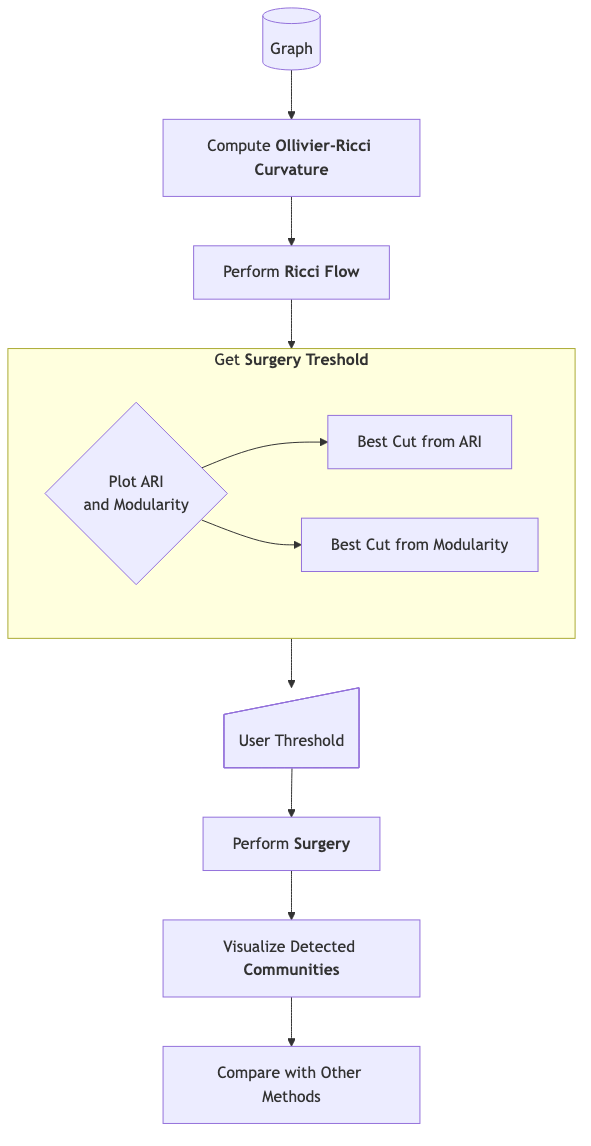
\includegraphics[width=0.7\textwidth]{Images/workflow.png}
    \caption{Code workflow.}
\end{figure}\label{fig:workflow}

%**************** TESTS FOR THE CODE ******************
\section{Tests on Synthetic Graphs}\label{sec5.2}
\subsection{Stochastic Block Model Test Graph}
To start testing our code we choose a Stochastic Block Model (SBM) graph. A SBM graph is a type of random graph model used to generate networks with a predefined community structure. It is an extension of the Erdos--R\'enyi, where nodes are divided into communities, and the probability of an edge between two nodes depends on their community membership. It is characterized by \textit{N} nodes, \textit{k} communities and a connectivity matrix \textit{$P_{ij}$} which represents the probability of an edge between a node in community $i$ and a node in community $j$.
Since communities are predefined when generating the graph, we can directly compare the detected communities with the true ones.

For our test we set 
\begin{equation*}
    N = 500, \quad k = 2, \quad
    P =
    \begin{bmatrix} 
        0.20 & 0.03 \\
        0.03 & 0.20
    \end{bmatrix}
\end{equation*}
with every initial weight equal to one.

Curvature values for the initial SBM graph are shown in fig.~\ref{fig:SBM_comparison_a}, while on the right we have the updated curvatures after 10 iterations of Ricci Flow. We can see that the community structure of this graph is already well established; Ricci Flow has however highlighted the weak connection of central inter community nodes as one can see in fig.~\ref{fig:SBM_comparison_b}.
\begin{figure}
    \centering
    \begin{subfigure}{0.45\textwidth}
        \centering
        \includegraphics[width=\textwidth]{../tests/ToyModelResults/SBM/Before Ricci Flow.png}
        \caption{Initial SBM graph, before Ricci Flow.}
        \label{fig:SBM_comparison_a}
    \end{subfigure}
    \hfill
    \begin{subfigure}{0.45\textwidth}
        \centering
        \includegraphics[width=\textwidth]{../tests/ToyModelResults/SBM/After Ricci Flow.png}
        \caption{SBM graph after Ricci Flow.}
        \label{fig:SBM_comparison_b}
    \end{subfigure}
    \caption{Comparison of SBM graph before and after having applied 10 iterations of Ricci Flow on edges.}
\end{figure}

In fig.~\ref{fig:SBM_Accuracy} we see that surgery with a cutoff between 1 and $\approx$1.5 leads to a perfect distinction between the two communities, i.e. an ARI of 1.

\begin{figure}
    \centering
    \includegraphics[width=0.6\textwidth]{../tests/ToyModelResults/SBM/Surgery Accuracy.png}
    \caption{SBM graph's ARI and modularity behavior for different surgery cutoffs.}
    \label{fig:SBM_Accuracy}
\end{figure}

Lastly, fig.~\ref{fig:SBM_Communities_a} depicts the graph after surgery with a cutoff between 1 and $\approx$1.5. As expected we got a separation into two distinct clusters. Fig.~\ref{fig:SBM_Communities_b} shows the two communities corresponding to the two connected components.
\begin{figure}
    \centering
    \begin{subfigure}{0.45\textwidth}
        \centering
        \includegraphics[width=\textwidth]{../tests/ToyModelResults/SBM/After Surgery.png}
        \caption{Final SBM graph, after surgery process.}
        \label{fig:SBM_Communities_a}
    \end{subfigure}
    \hfill
    \begin{subfigure}{0.45\textwidth}
        \centering
        
\includegraphics[width=\textwidth]{../tests/ToyModelResults/SBM/Detected Communities.png}
        \caption{Detected communities after surgery on SBM graph.}
        \label{fig:SBM_Communities_b}
    \end{subfigure}
    \caption{Comparison of SBM graph after surgery and corresponding connected components (i.e. the detected communities).}
\end{figure}


\subsection{Lancichinetti-Fortunato-Radicchi Test Graph}
As a more complex synthetic graph for testing we used a Lancichinetti-Fortunato-Radicchi (LFR) benchmark graph. LFR graphs are widely used for testing community-detection algorithms because they produce networks with heterogeneous (scale-free) degree distributions and community-size distributions, making them more realistic than simpler models. Nodes are assigned to communities according to specified power-law exponents, and a “mixing” parameter controls the fraction of edges that connect different communities.

For our test we built a graph with 500 nodes \(\bigl(n = 500\bigr)\) with a degree distribution exponent \(\tau_{1} = 3\) and a community-size exponent \(\tau_{2} = 1.5\). For the mixing parameter we chose \(\mu = 0.2\) indicates a relatively strong community structure by limiting the proportion of inter-community edges. We set each community to have a minimum of 20 nodes and a maximum of 70 nodes. The expected average degree is set to 20, with a maximum node degree capped at 50. 

For this graph we applied 40 iterations of Ricci Flow as its structure is more complex than the previous SBM graph (see fig.~\ref{fig:LFR_comparison_a}). In fig.~\ref{fig:LFR_comparison_b} we see a covergence of the curvature values after Ricci Flow; the high number of nodes and communities makes difficult to visualize properly the graph, for this reason we introduced also an histogram plot of weights and curvature values in the final code implementation for the Karate club graph (see \autoref{sec5.3}).
\begin{figure}
    \centering
    \begin{subfigure}{0.45\textwidth}
        \centering
        \includegraphics[width=\textwidth]{../tests/ToyModelResults/LFR/Before Ricci Flow.png}
        \caption{Initial LFR graph, before Ricci Flow.}
        \label{fig:LFR_comparison_a}
    \end{subfigure}
    \hfill
    \begin{subfigure}{0.45\textwidth}
        \centering
        \includegraphics[width=\textwidth]{../tests/ToyModelResults/LFR/After Ricci Flow.png}
        \caption{LFR graph after Ricci Flow.}
        \label{fig:LFR_comparison_b}
    \end{subfigure}
    \caption{Comparison of LFR graph before and after having applied 40 iterations of  Ricci Flow on edges.}
\end{figure}

Fig.~\ref{fig:LFR_Accuracy} shows the behavior of ARI and modularity depending on the choosen cutoff point. Also in this case we see that it is possible to obtain an ARI of 1.
\begin{figure}
    \centering
    \includegraphics[width=0.6\textwidth]{../tests/ToyModelResults/LFR/Surgery Accuracy.png}
    \caption{LFR graph's ARI and modularity behavior for different surgery cutoffs.}
    \label{fig:LFR_Accuracy}
\end{figure}

In fig.~\ref{fig:LFR_Surgery} we have the graph after surgery (we chose as cutoff $\approx$1.12 to get an ARI of 1) and we can see that it got divided into connected components with all the nodes of the same color, i.e. same community. In this case we did not produce a plot community by community due to the high number of clusters. 
\begin{figure}
    \centering
    \includegraphics[width=0.6\textwidth]{../tests/ToyModelResults/LFR/After Surgery.png}
        \caption{Final LFR graph, after surgery process.}
        \label{fig:LFR_Surgery}
\end{figure}

\subsection{Further Tests on Lancichinetti-Fortunato-Radicchi Graphs}
As a final test for our code we decided to try reproducing a result presented in the work of Ni et al. \cite{Ni:communitydetectionnetworksricci} (see \textit{figure 8a} at page 12). In particular, it is about applying Ricci Flow on different LFR graphs differing for the modularity parameter $\mu$. Of course one expects the ARI to decrease with increasing values of $\mu$ as the community structure becomes less defined.

In fig.~\ref{fig:LFR_OTD} we present our results with OTD method for curvature evaluation
\begin{figure}
    \centering
    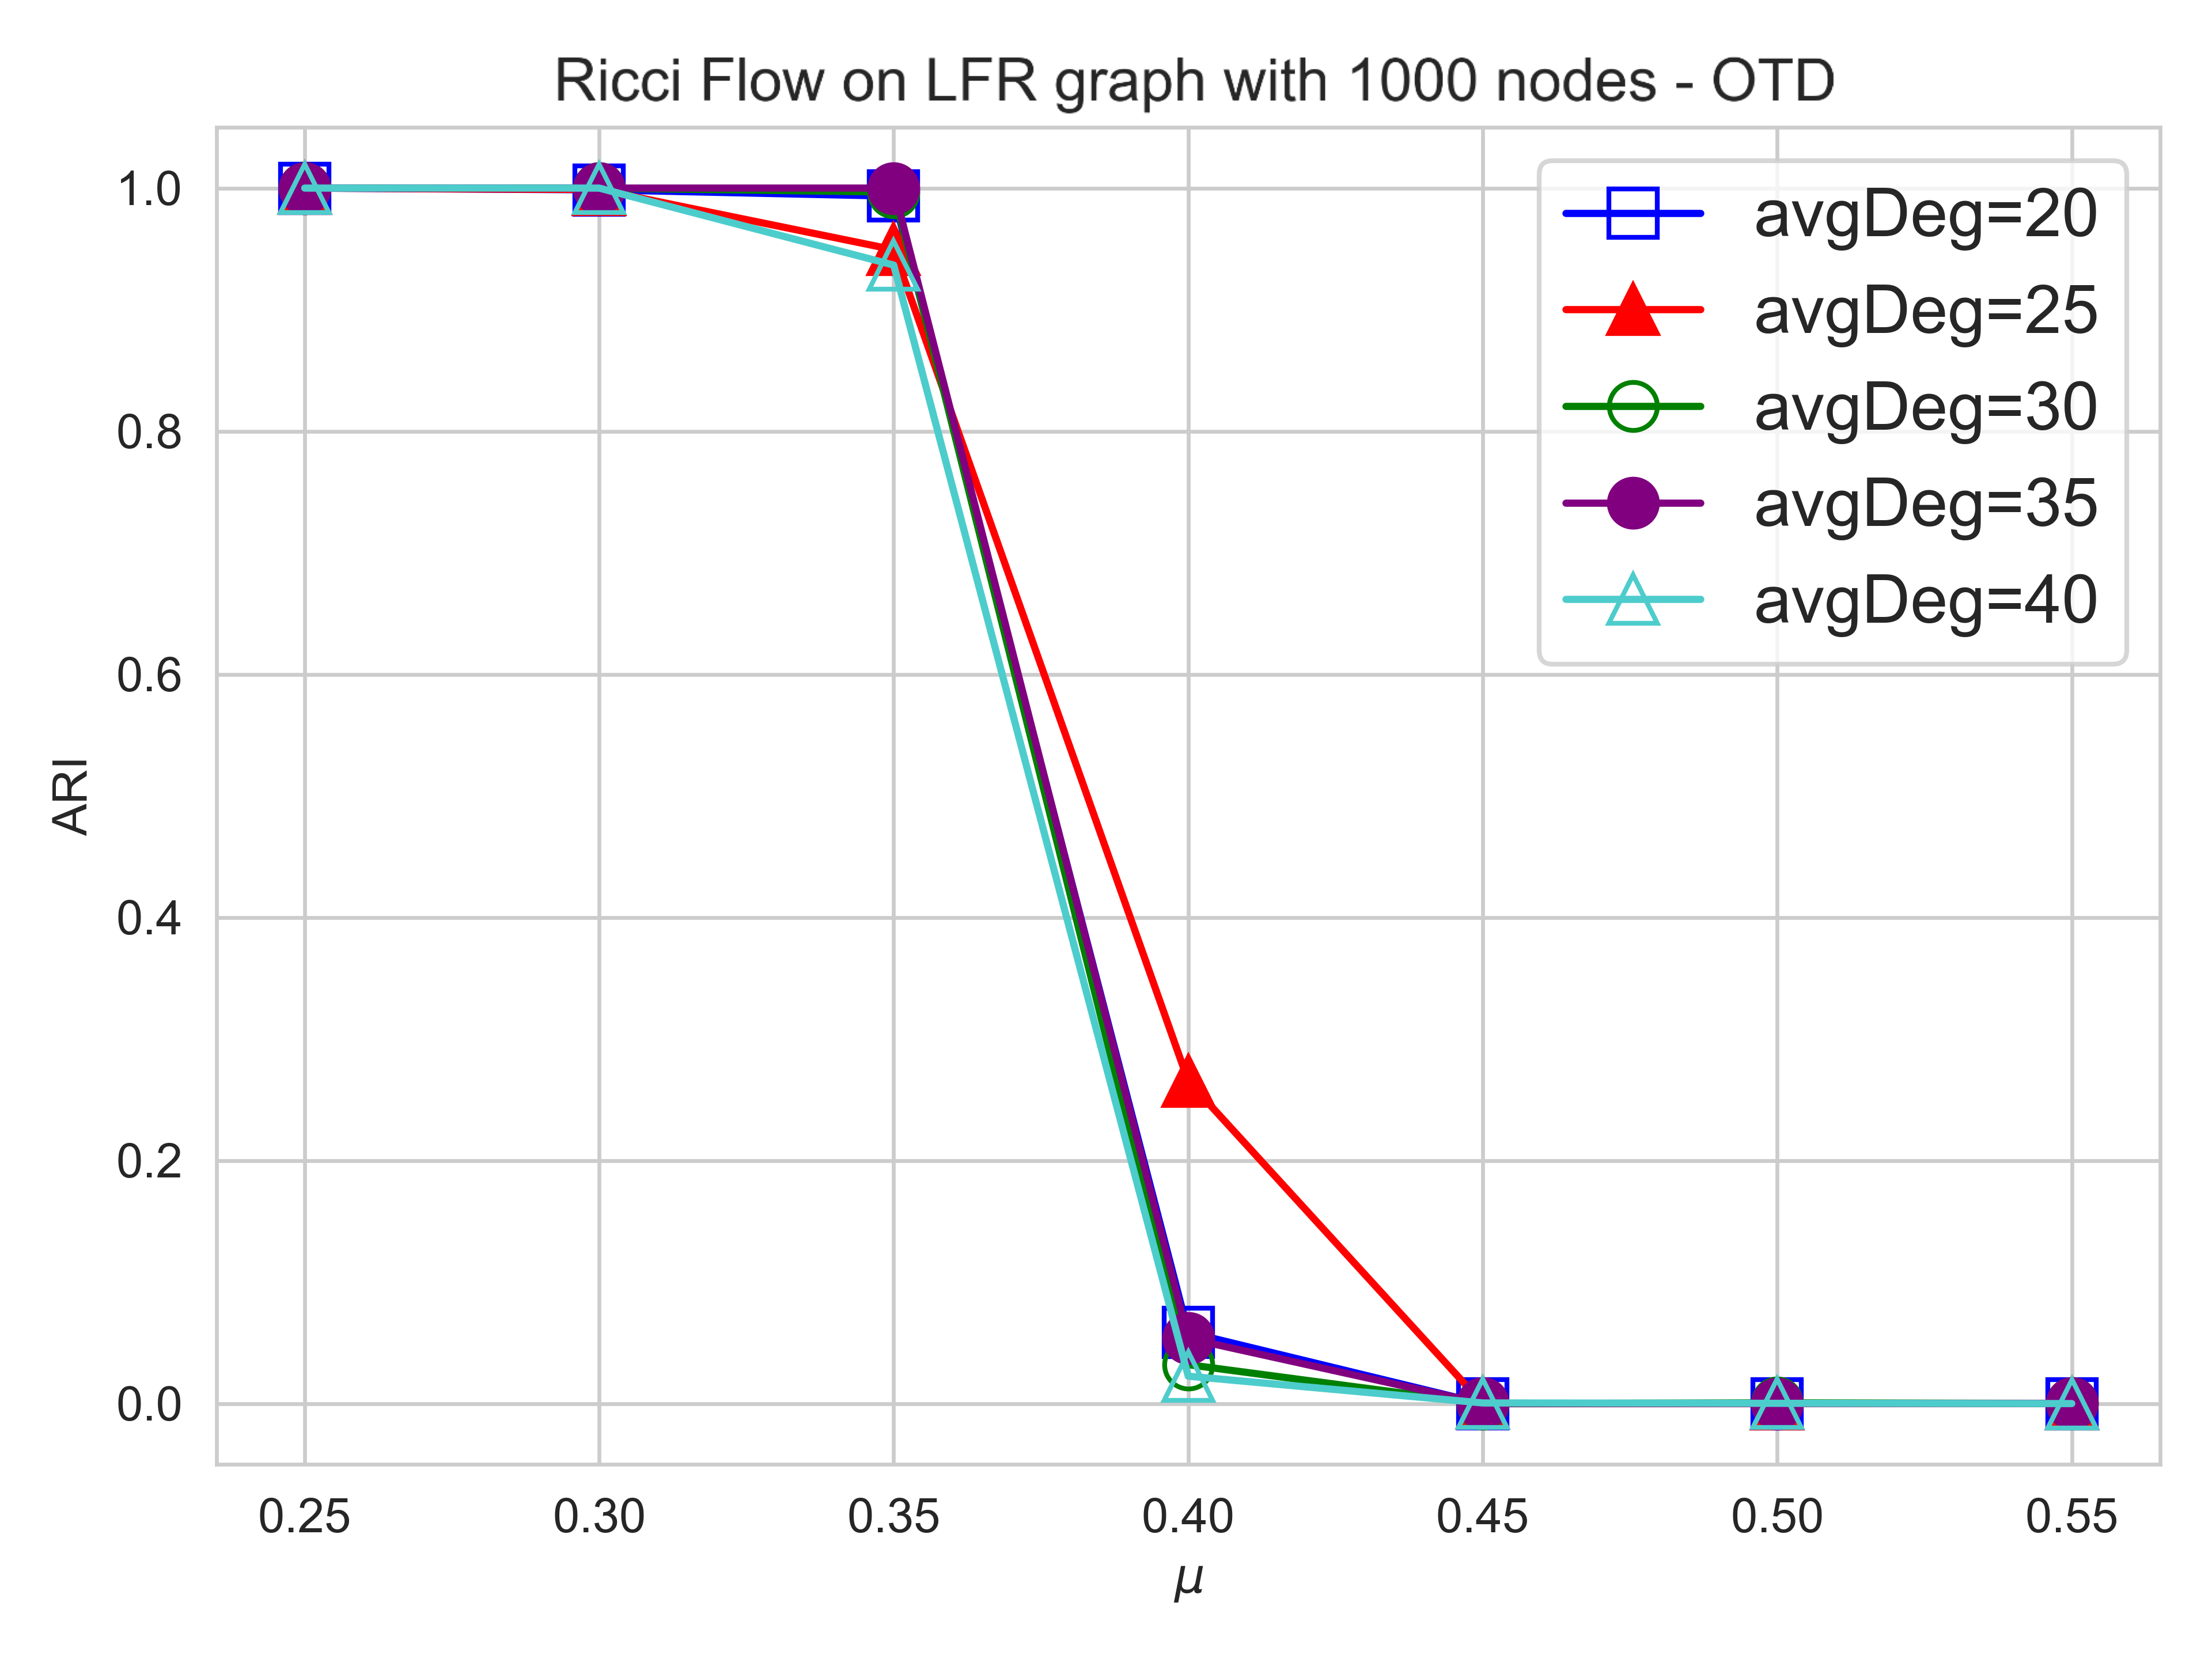
\includegraphics[width=0.6\textwidth]{../tests/LFRResults/LFR_OTD.png}
    \caption{LFR OTD}
    \label{fig:LFR_OTD}
\end{figure}

using first OTD and then ATD
\begin{figure}
    \centering
    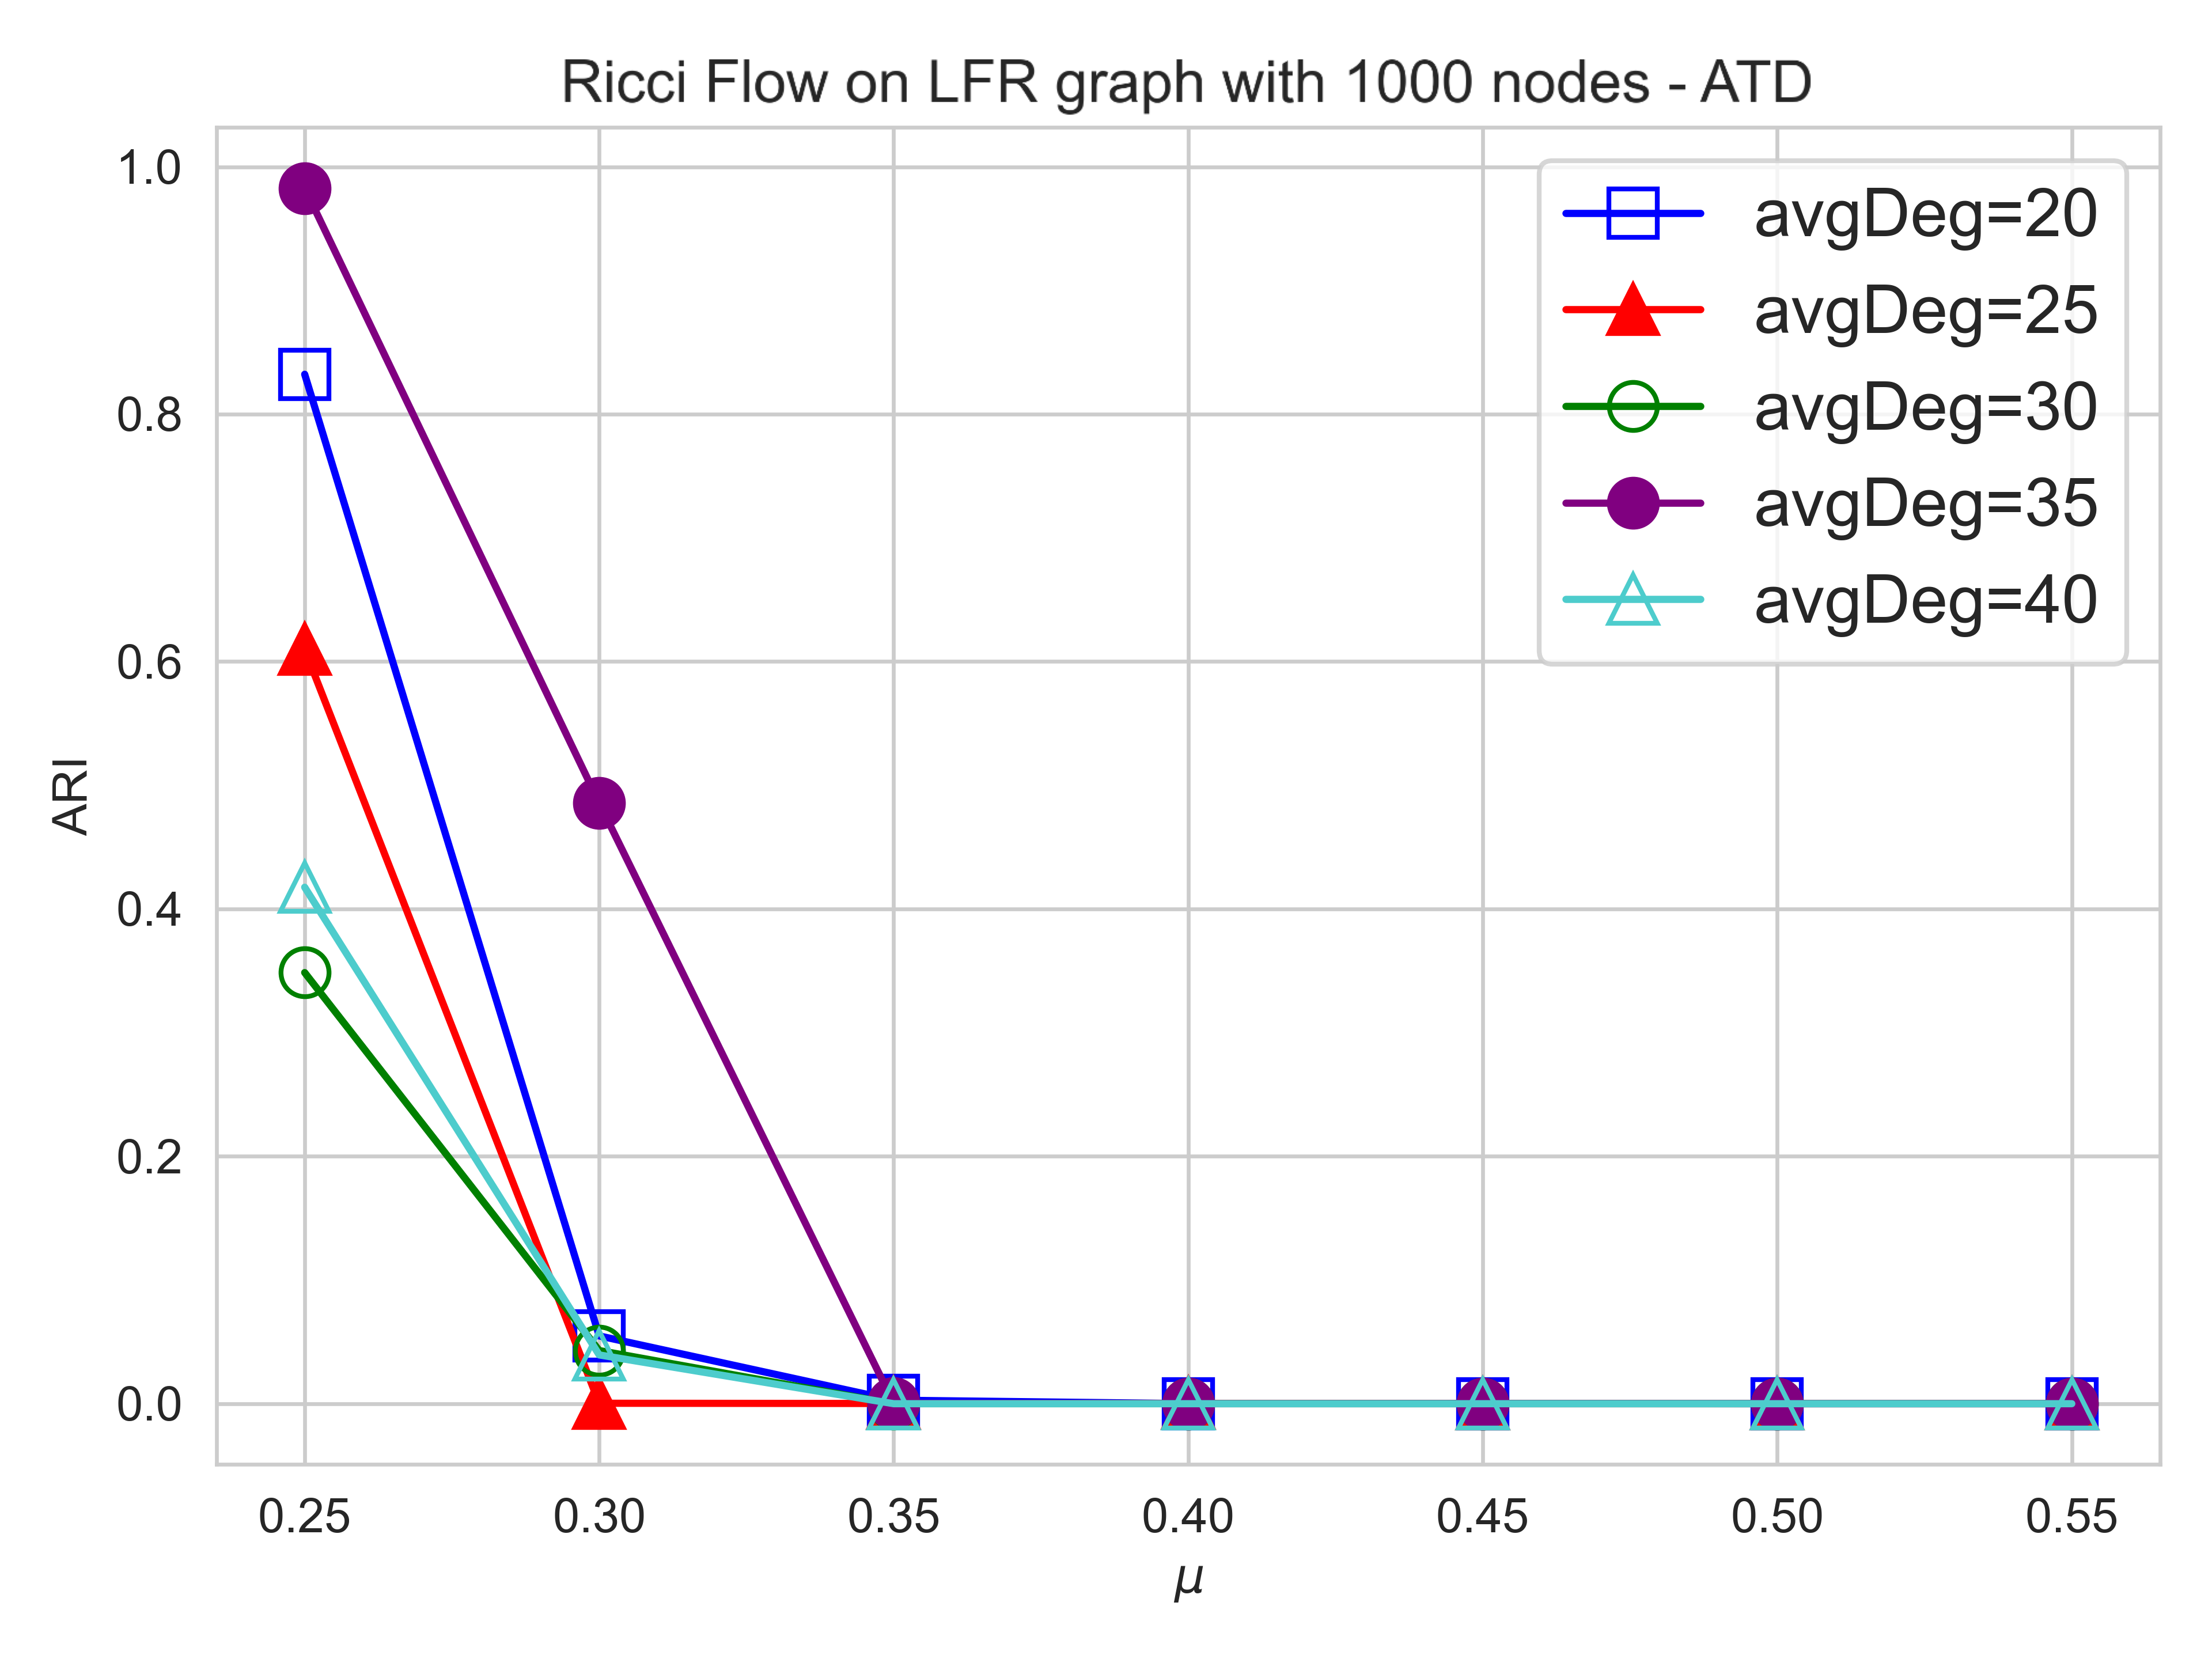
\includegraphics[width=0.6\textwidth]{../tests/LFRResults/LFR_ATD.png}
    \caption{LFR ATD}
    \label{fig:LFR_ATD}
\end{figure}

Our graphs do not match exactly the plots of Ni et al., as for them the loss of ARI starts from higher values of $\mu$. This could be for various reasons:
\begin{itemize}
    \item It is unclear which parameter they used to generate LFR graphs. For example, using Networkx it is not possible to control exactly the number of communities (only a minimum and maximum number can be set), so they probably generated their graphs in a different but unspecified way.
    \item They used an average ARI, probably generating the same graph multiple times. We generated the graph and applied the Ricci Flow just once due to an already high execution time.
    \item Their surgery process it is not specified in detail. They might have used multiple surgeries over the same Ricci Flow process to remove possible singularities affecting the final performance (even though this should not be the case for this kind of graph).
\end{itemize}
%**************** KARATE CLUB DATASET APPLICATION ******************
\section{Application to Zachary's Karate Club Graph}
\label{sec5.3}

\begin{figure}
    \centering
    \begin{subfigure}{0.45\textwidth}
        \centering
        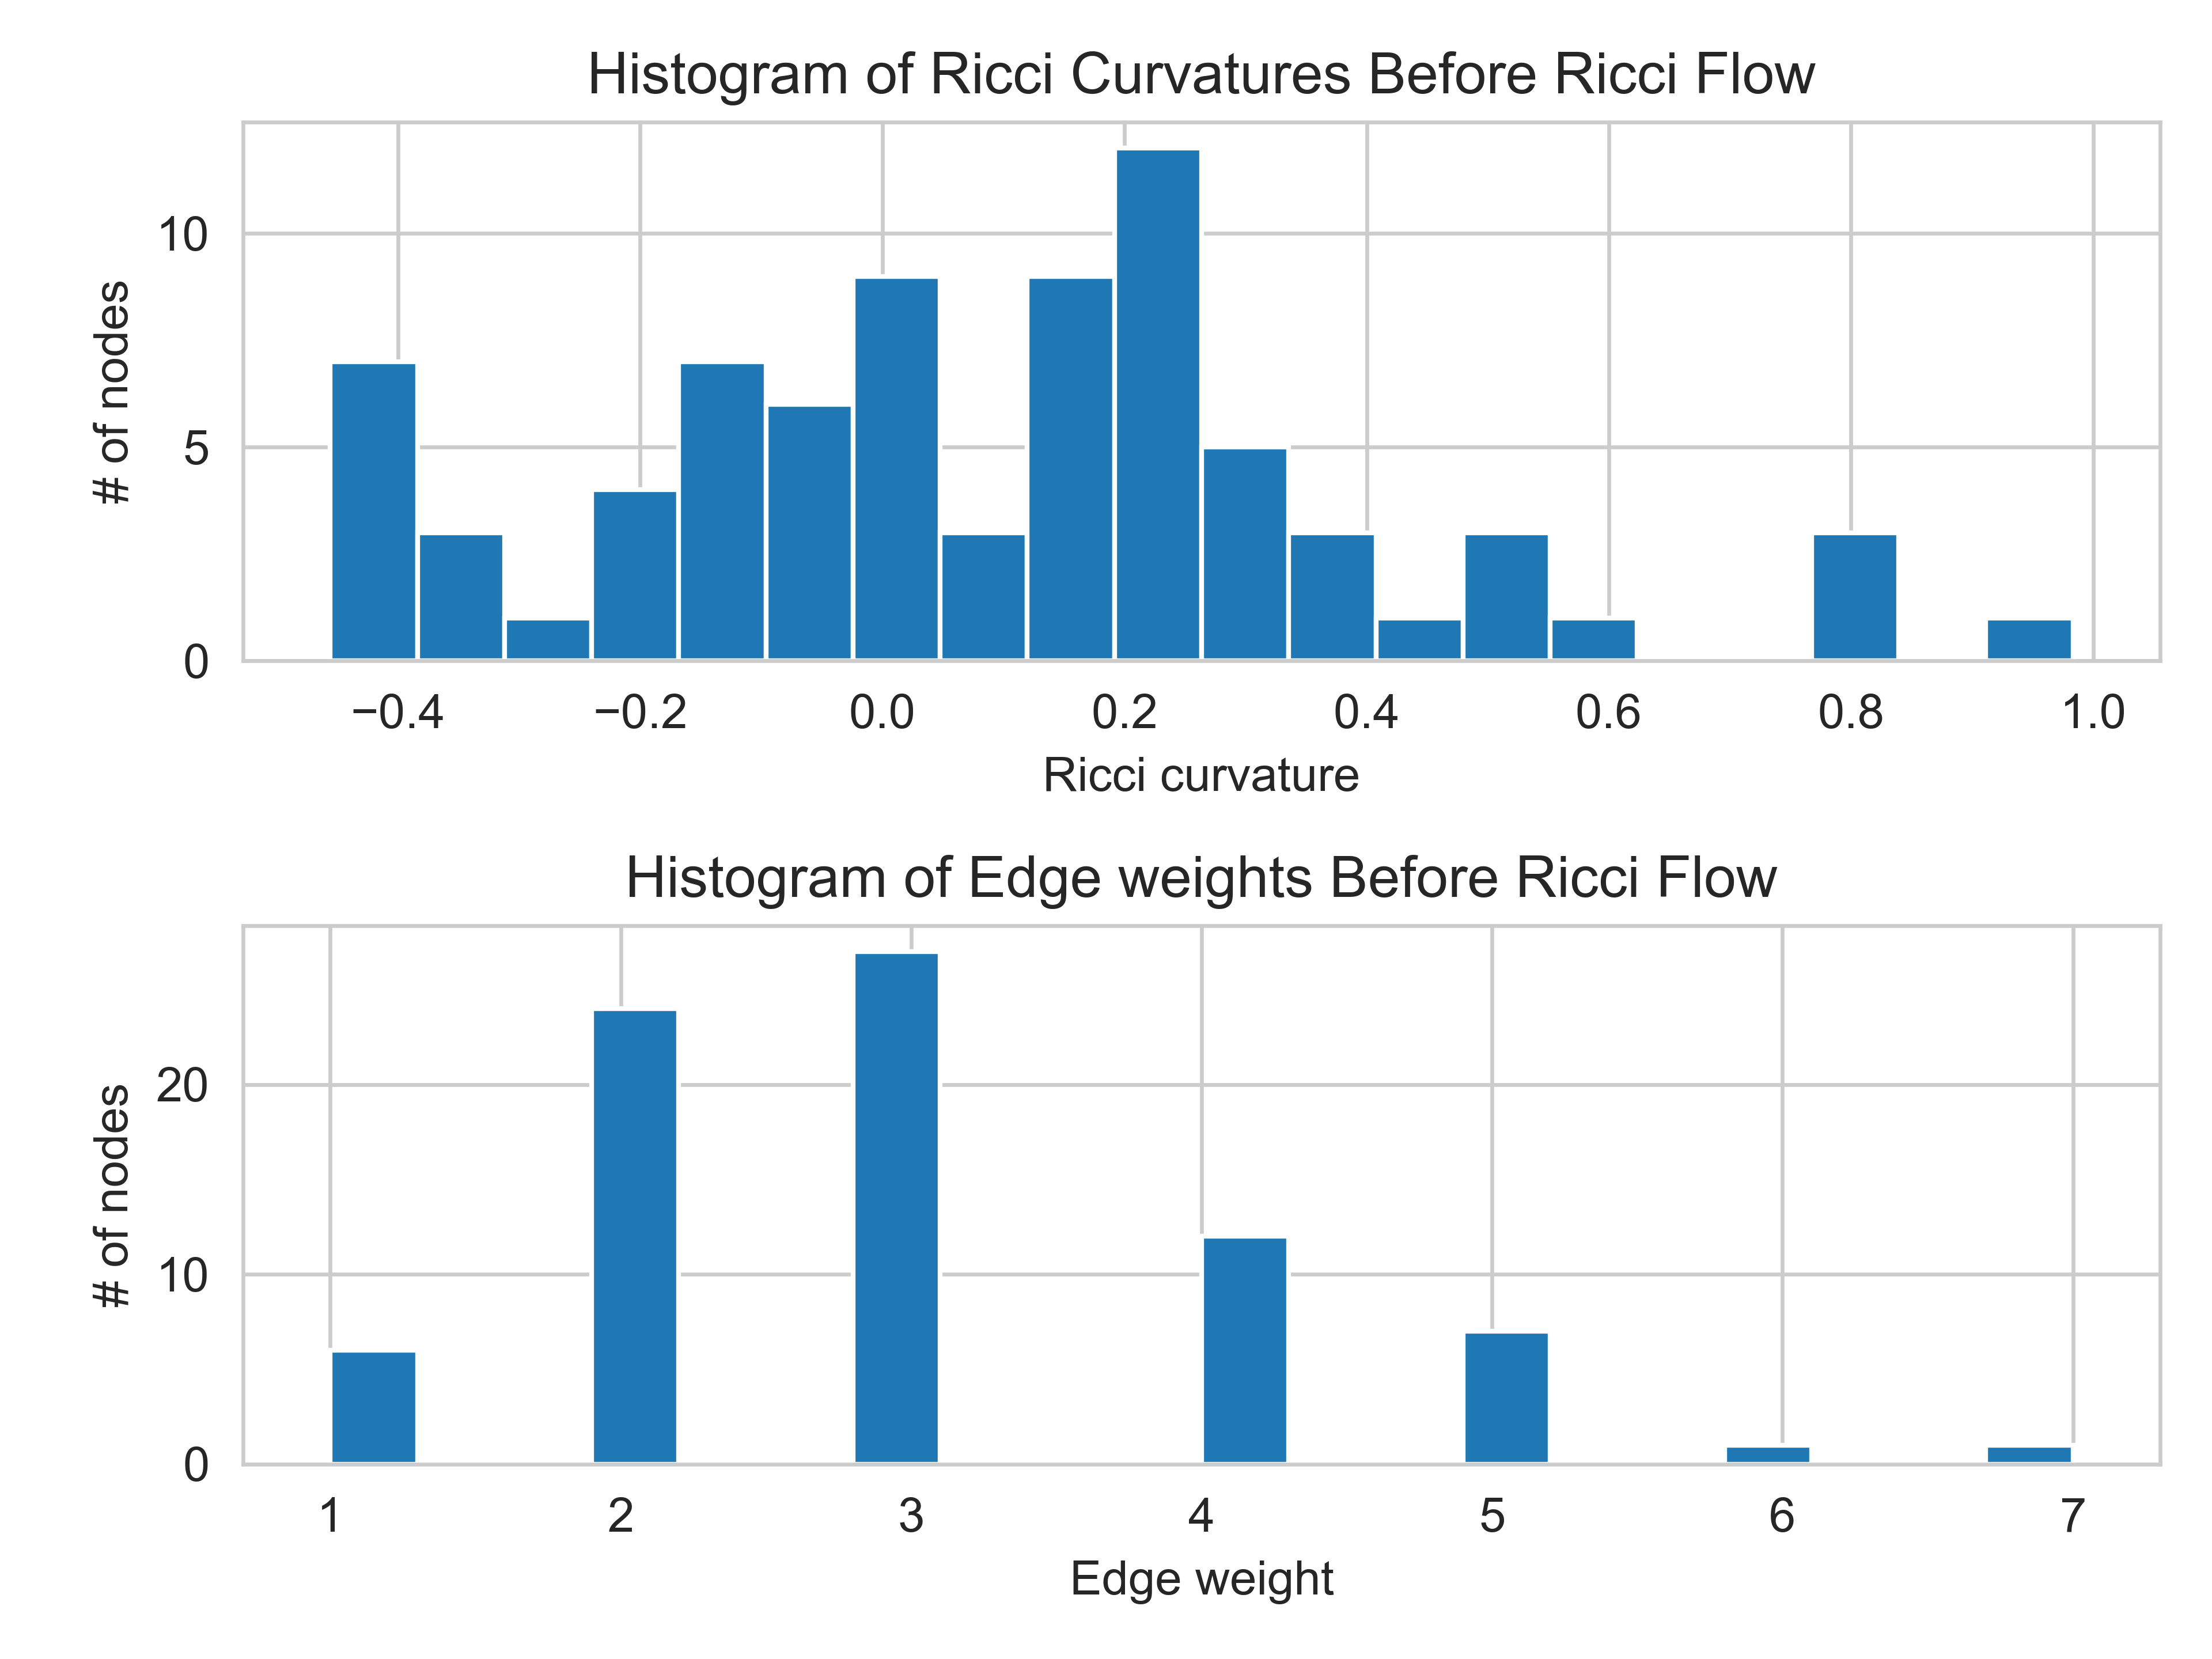
\includegraphics[width=\textwidth]{../KarateClubResults/Before Ricci Flow.png}
        \caption{Initial Karate graph, before Ricci Flow.}
        \label{fig:Karate_Before_Ricci_flow_histo}
    \end{subfigure}
    \hfill
    \begin{subfigure}{0.45\textwidth}
        \centering
        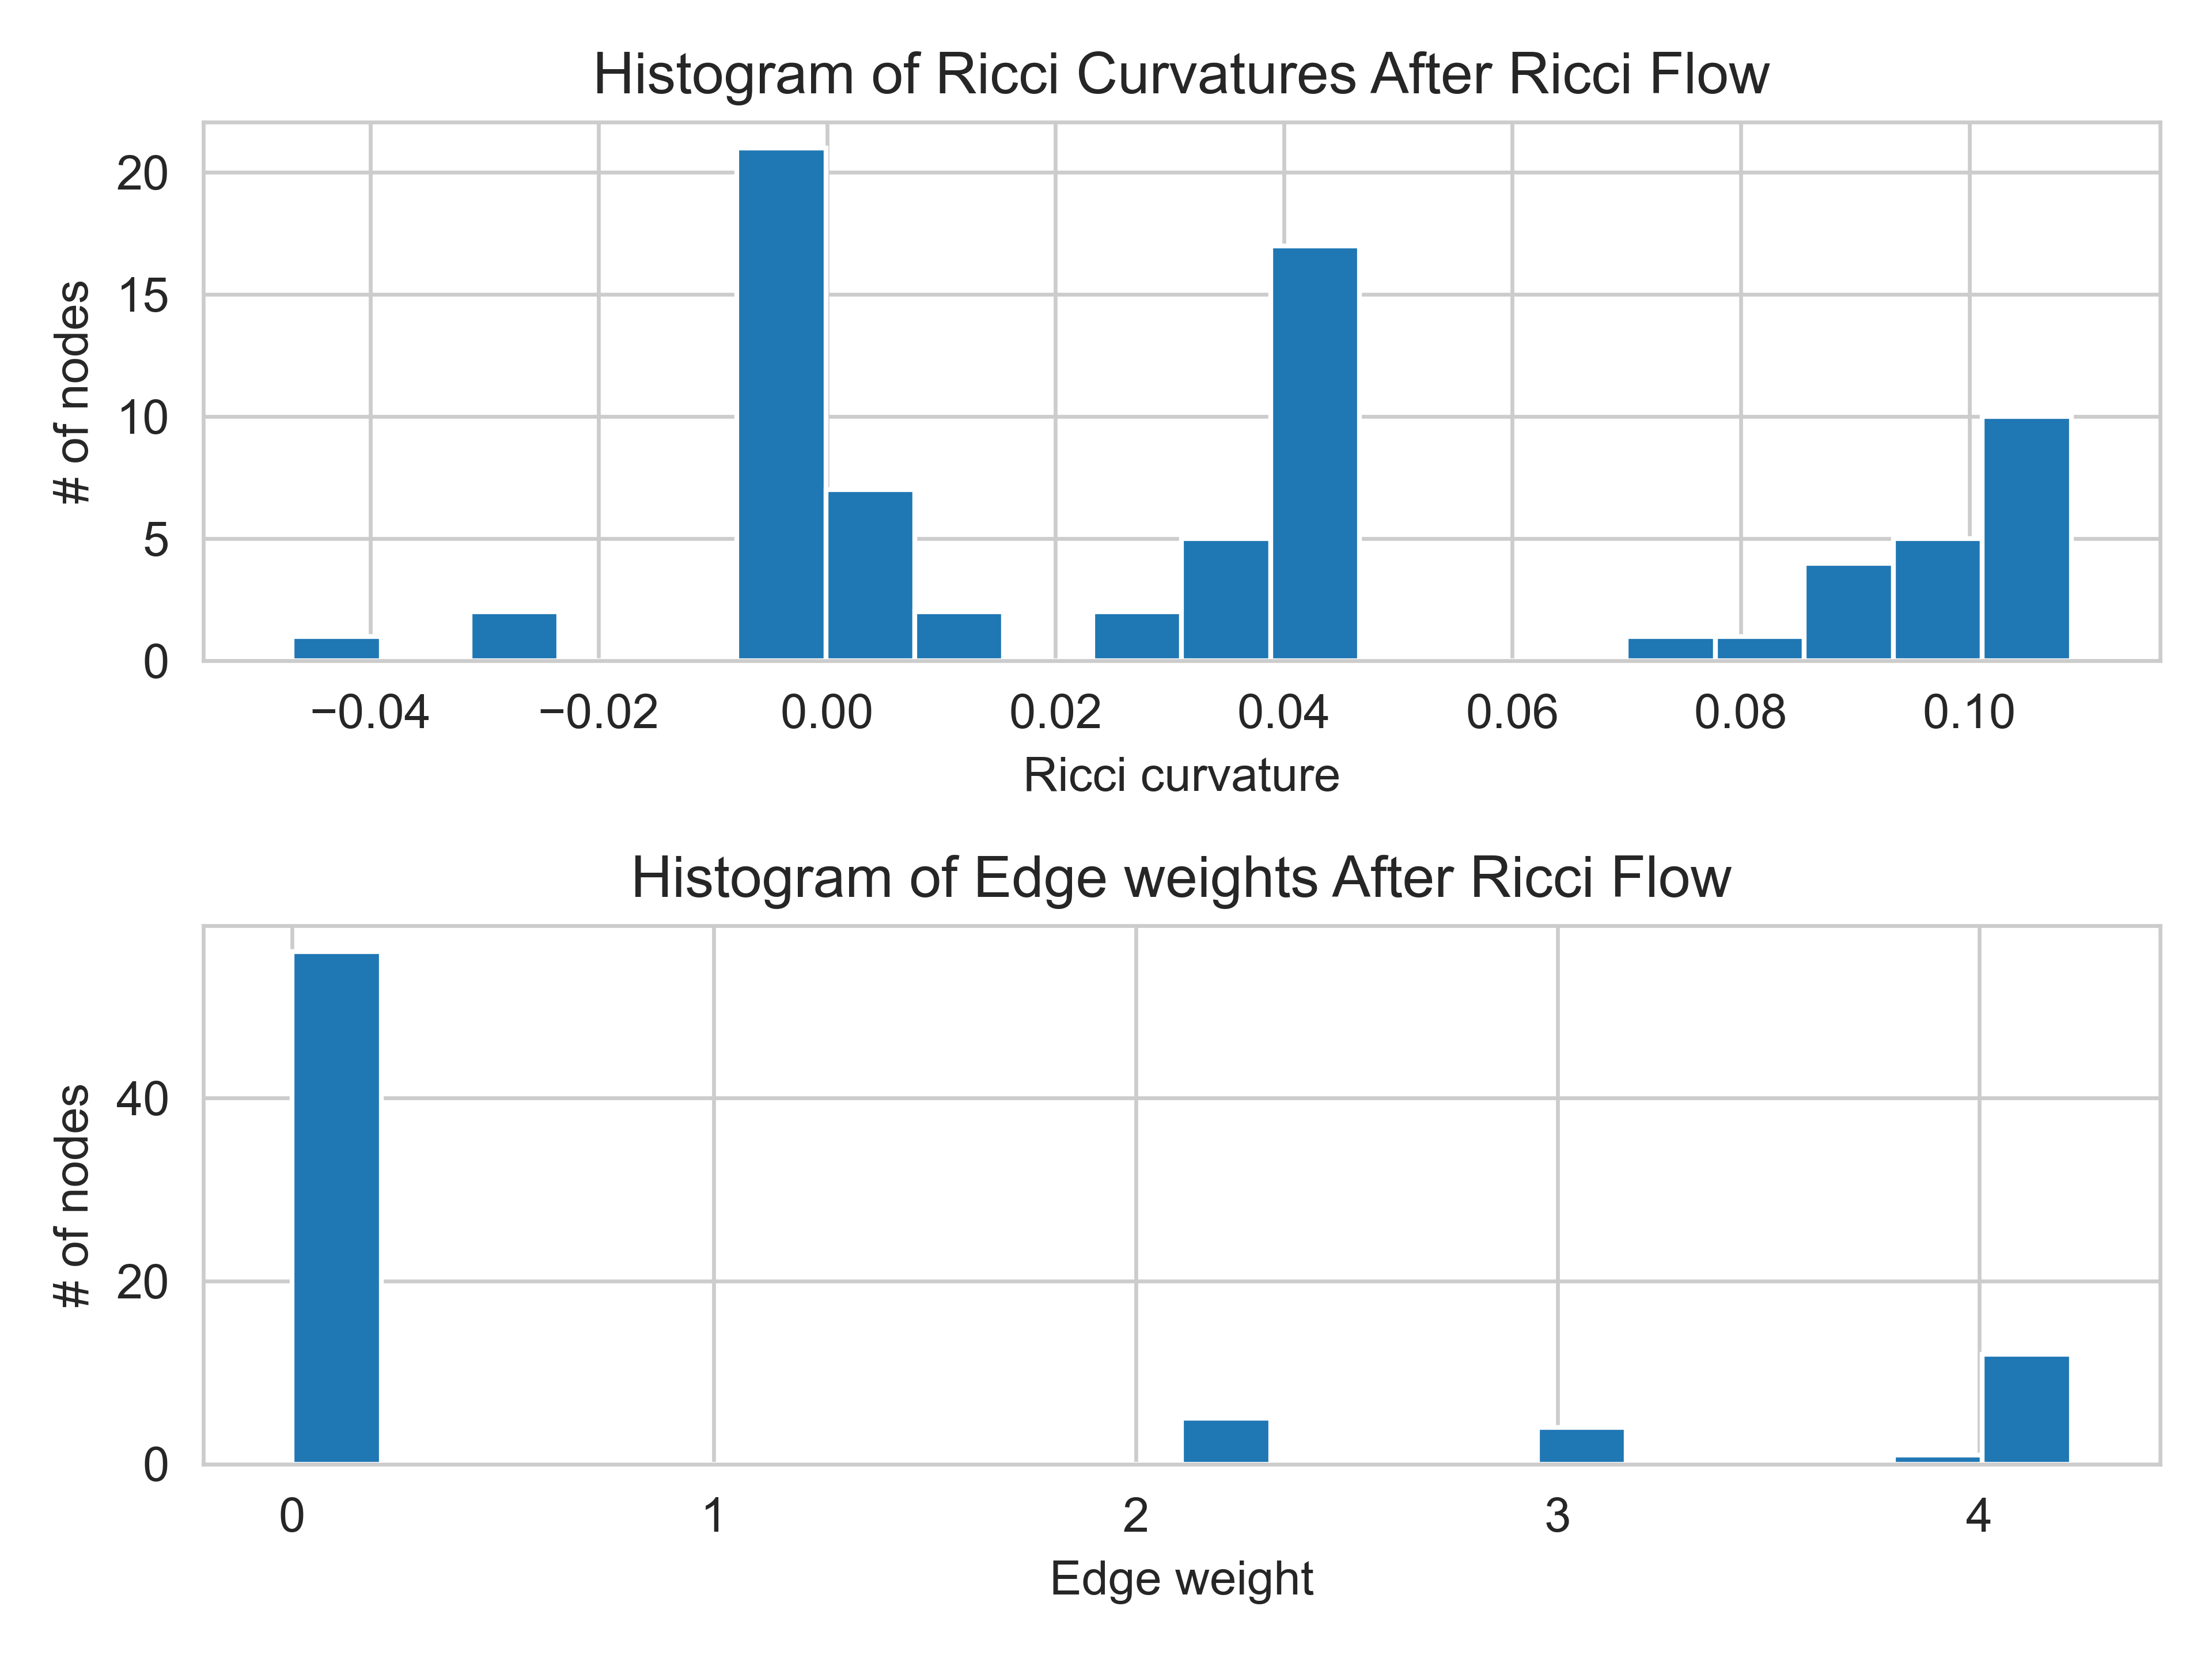
\includegraphics[width=\textwidth]{../KarateClubResults/After Ricci Flow.png}
        \caption{Karate graph after Ricci Flow.}
        \label{fig:Karate_After_Ricci_flow_histo}
    \end{subfigure}
    \caption{Comparison of curvature values and weights before and after having applied Ricci Flow on edges.}
    \label{fig:Karate_comparison_histo}
\end{figure}

\begin{figure}
    \centering
    \begin{subfigure}{0.45\textwidth}
        \centering
        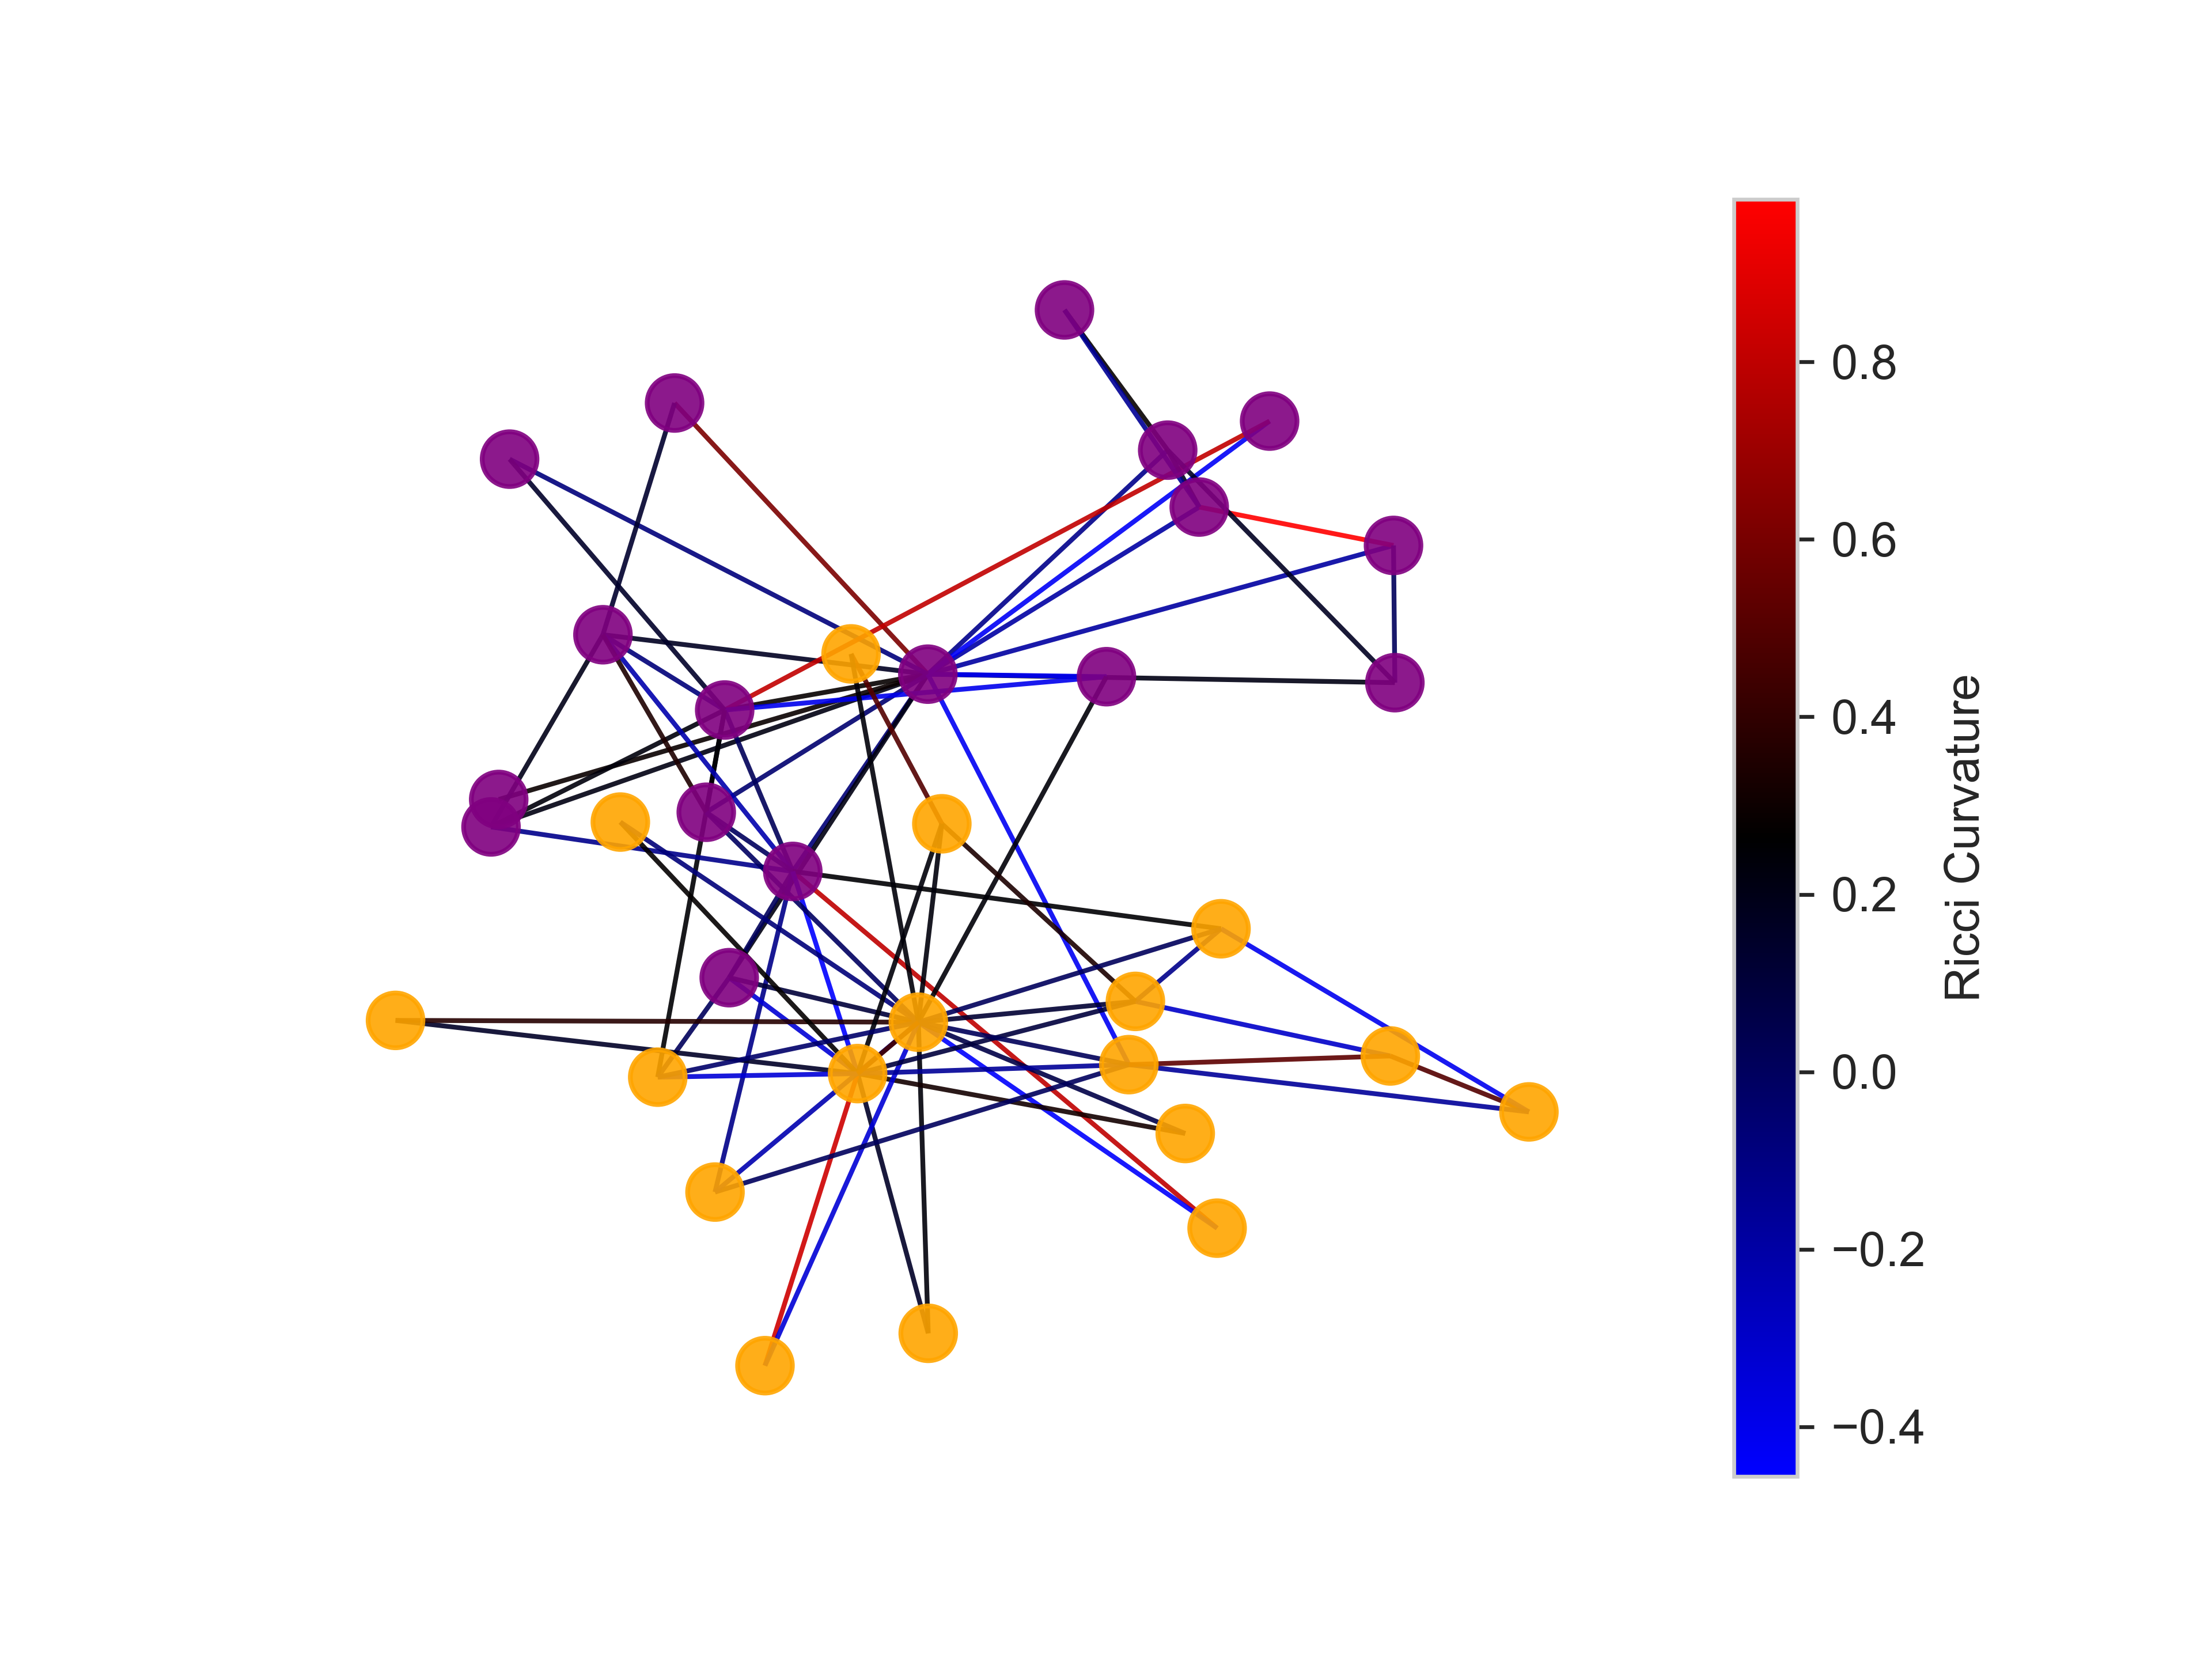
\includegraphics[width=\textwidth]{../KarateClubResults/Before Ricci Flow (graph).png}
        \caption{Initial Karate graph, before Ricci Flow.}
        \label{fig:Karate_Before_Ricci_flow_graphs}
    \end{subfigure}
    \hfill
    \begin{subfigure}{0.45\textwidth}
        \centering
        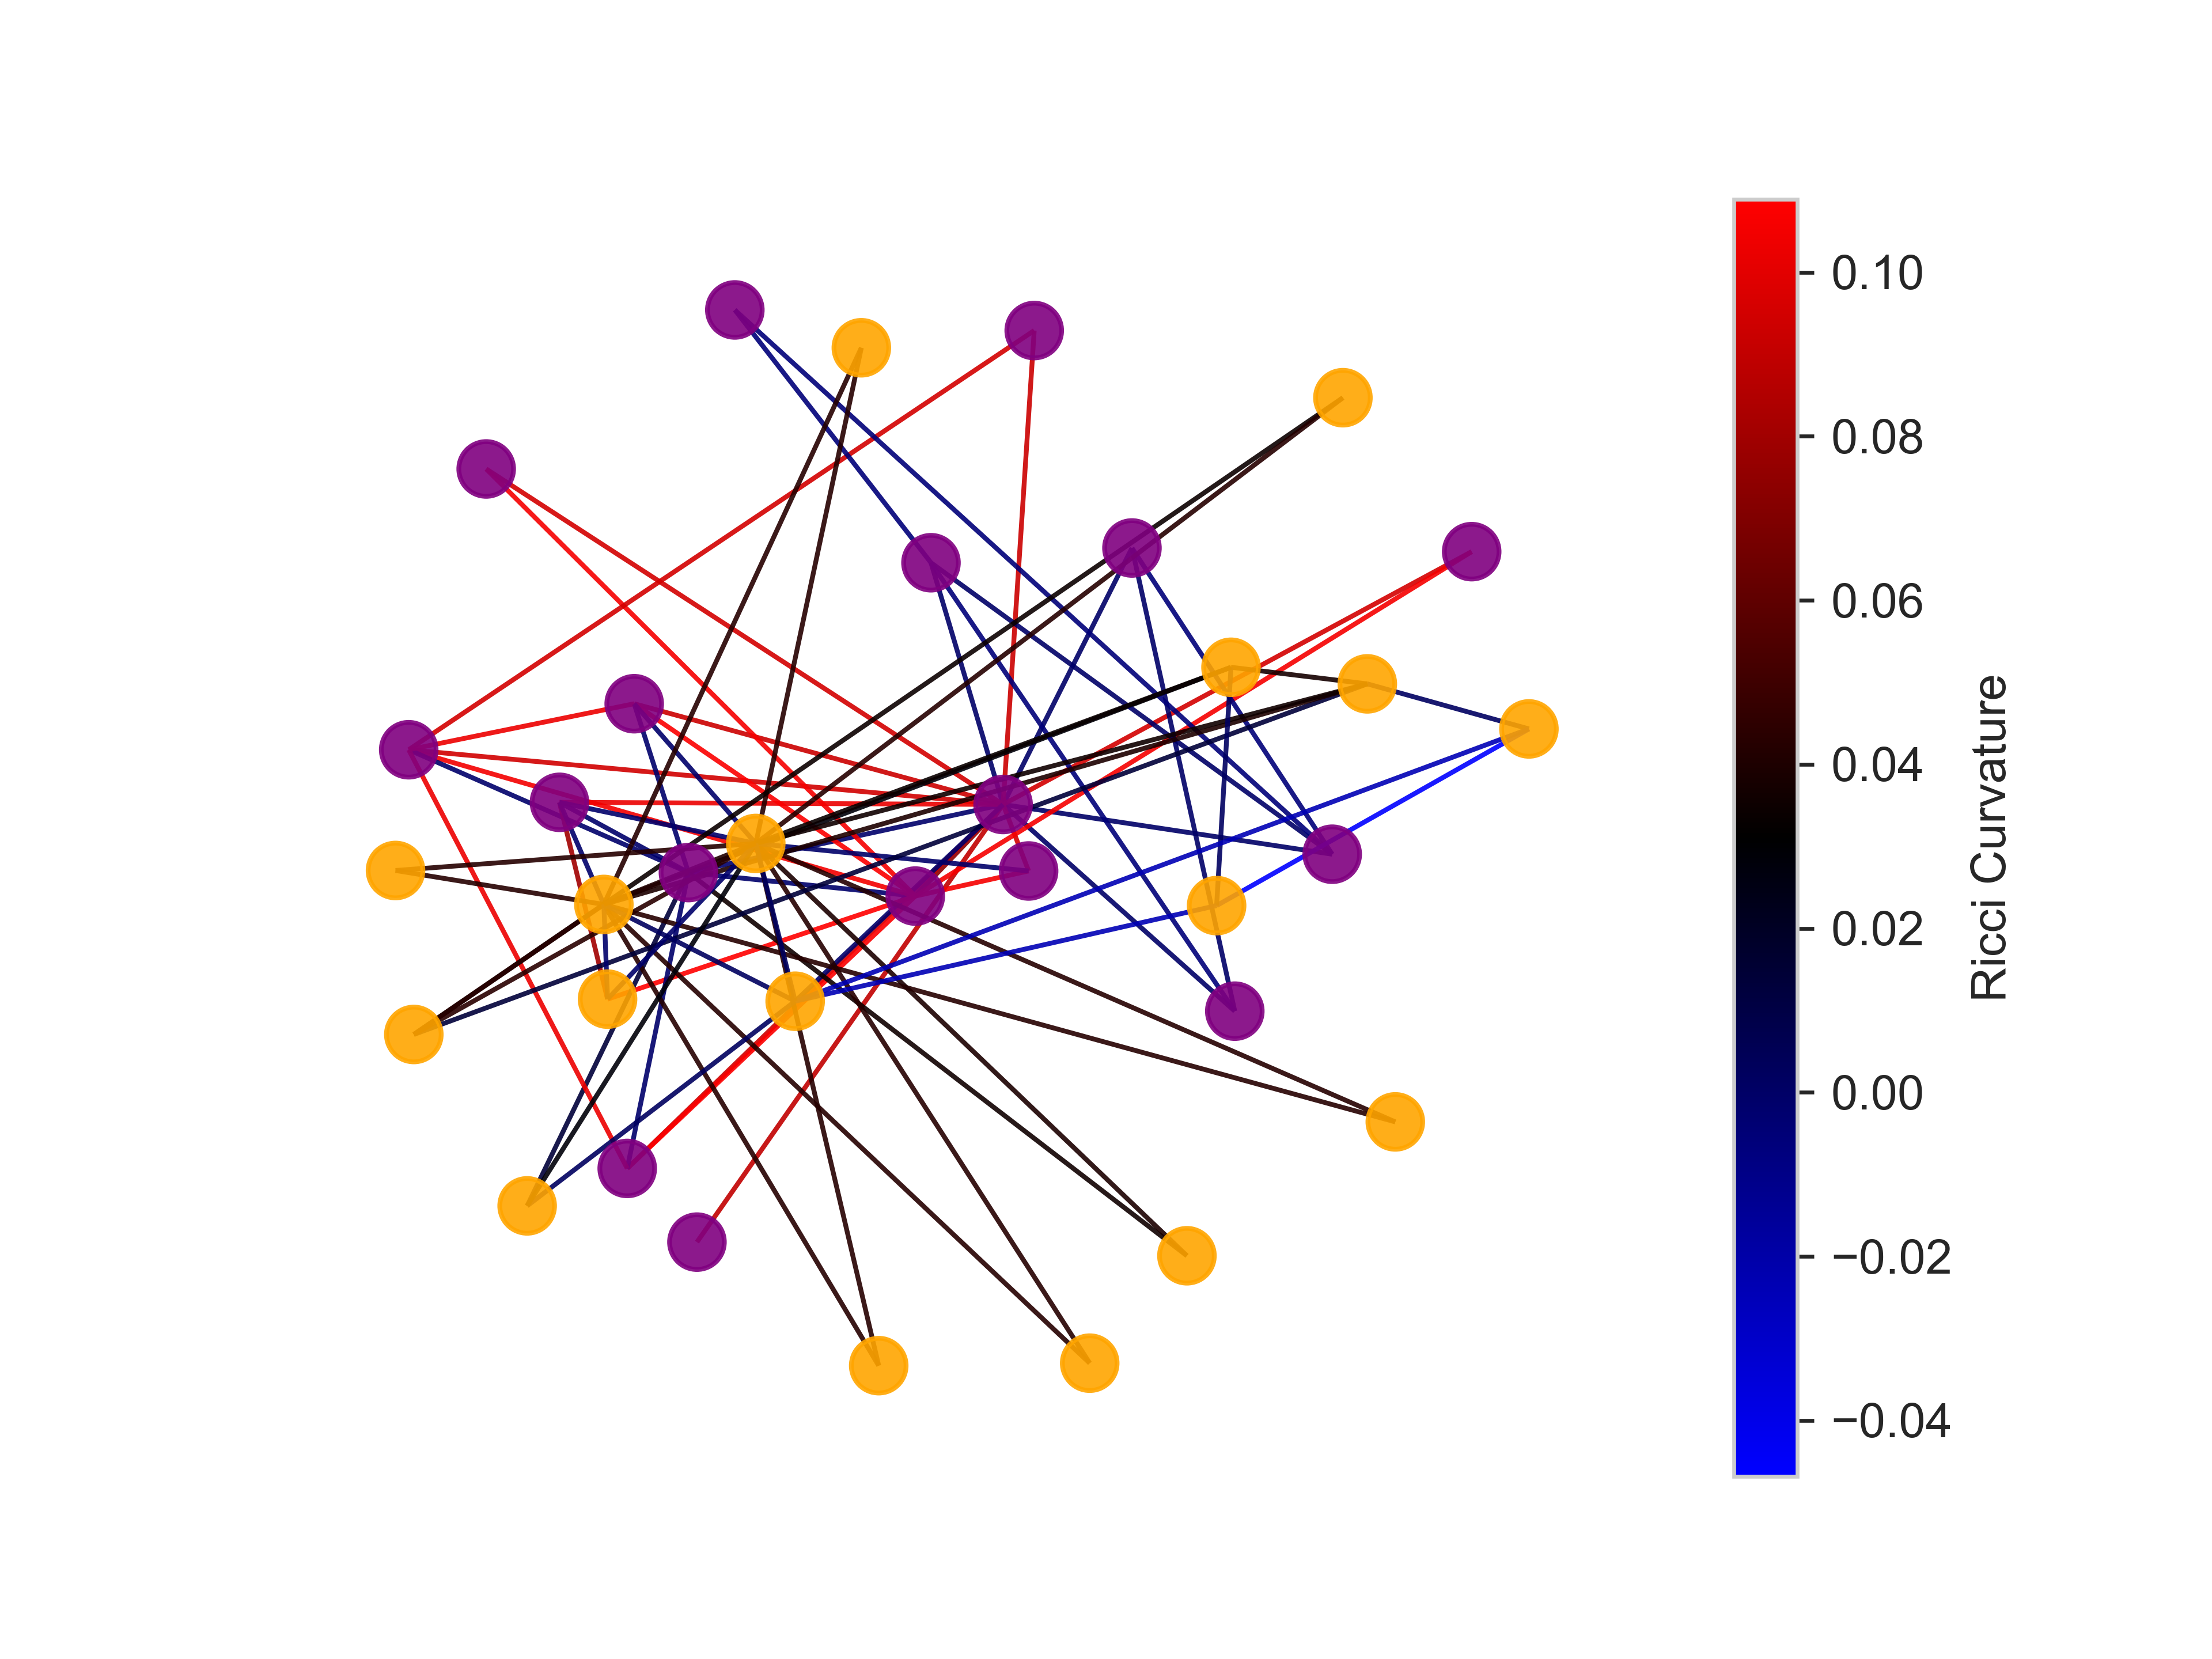
\includegraphics[width=\textwidth]{../KarateClubResults/After Ricci Flow (graph).png}
        \caption{Karate graph after Ricci Flow.}
        \label{fig:Karate_After_Ricci_flow_graphs}
    \end{subfigure}
    \caption{Comparison of Karate graph before and after having applied Ricci Flow on edges.}
    \label{fig:Karate_comparison_graphs}
\end{figure}

\begin{figure}
    \centering
    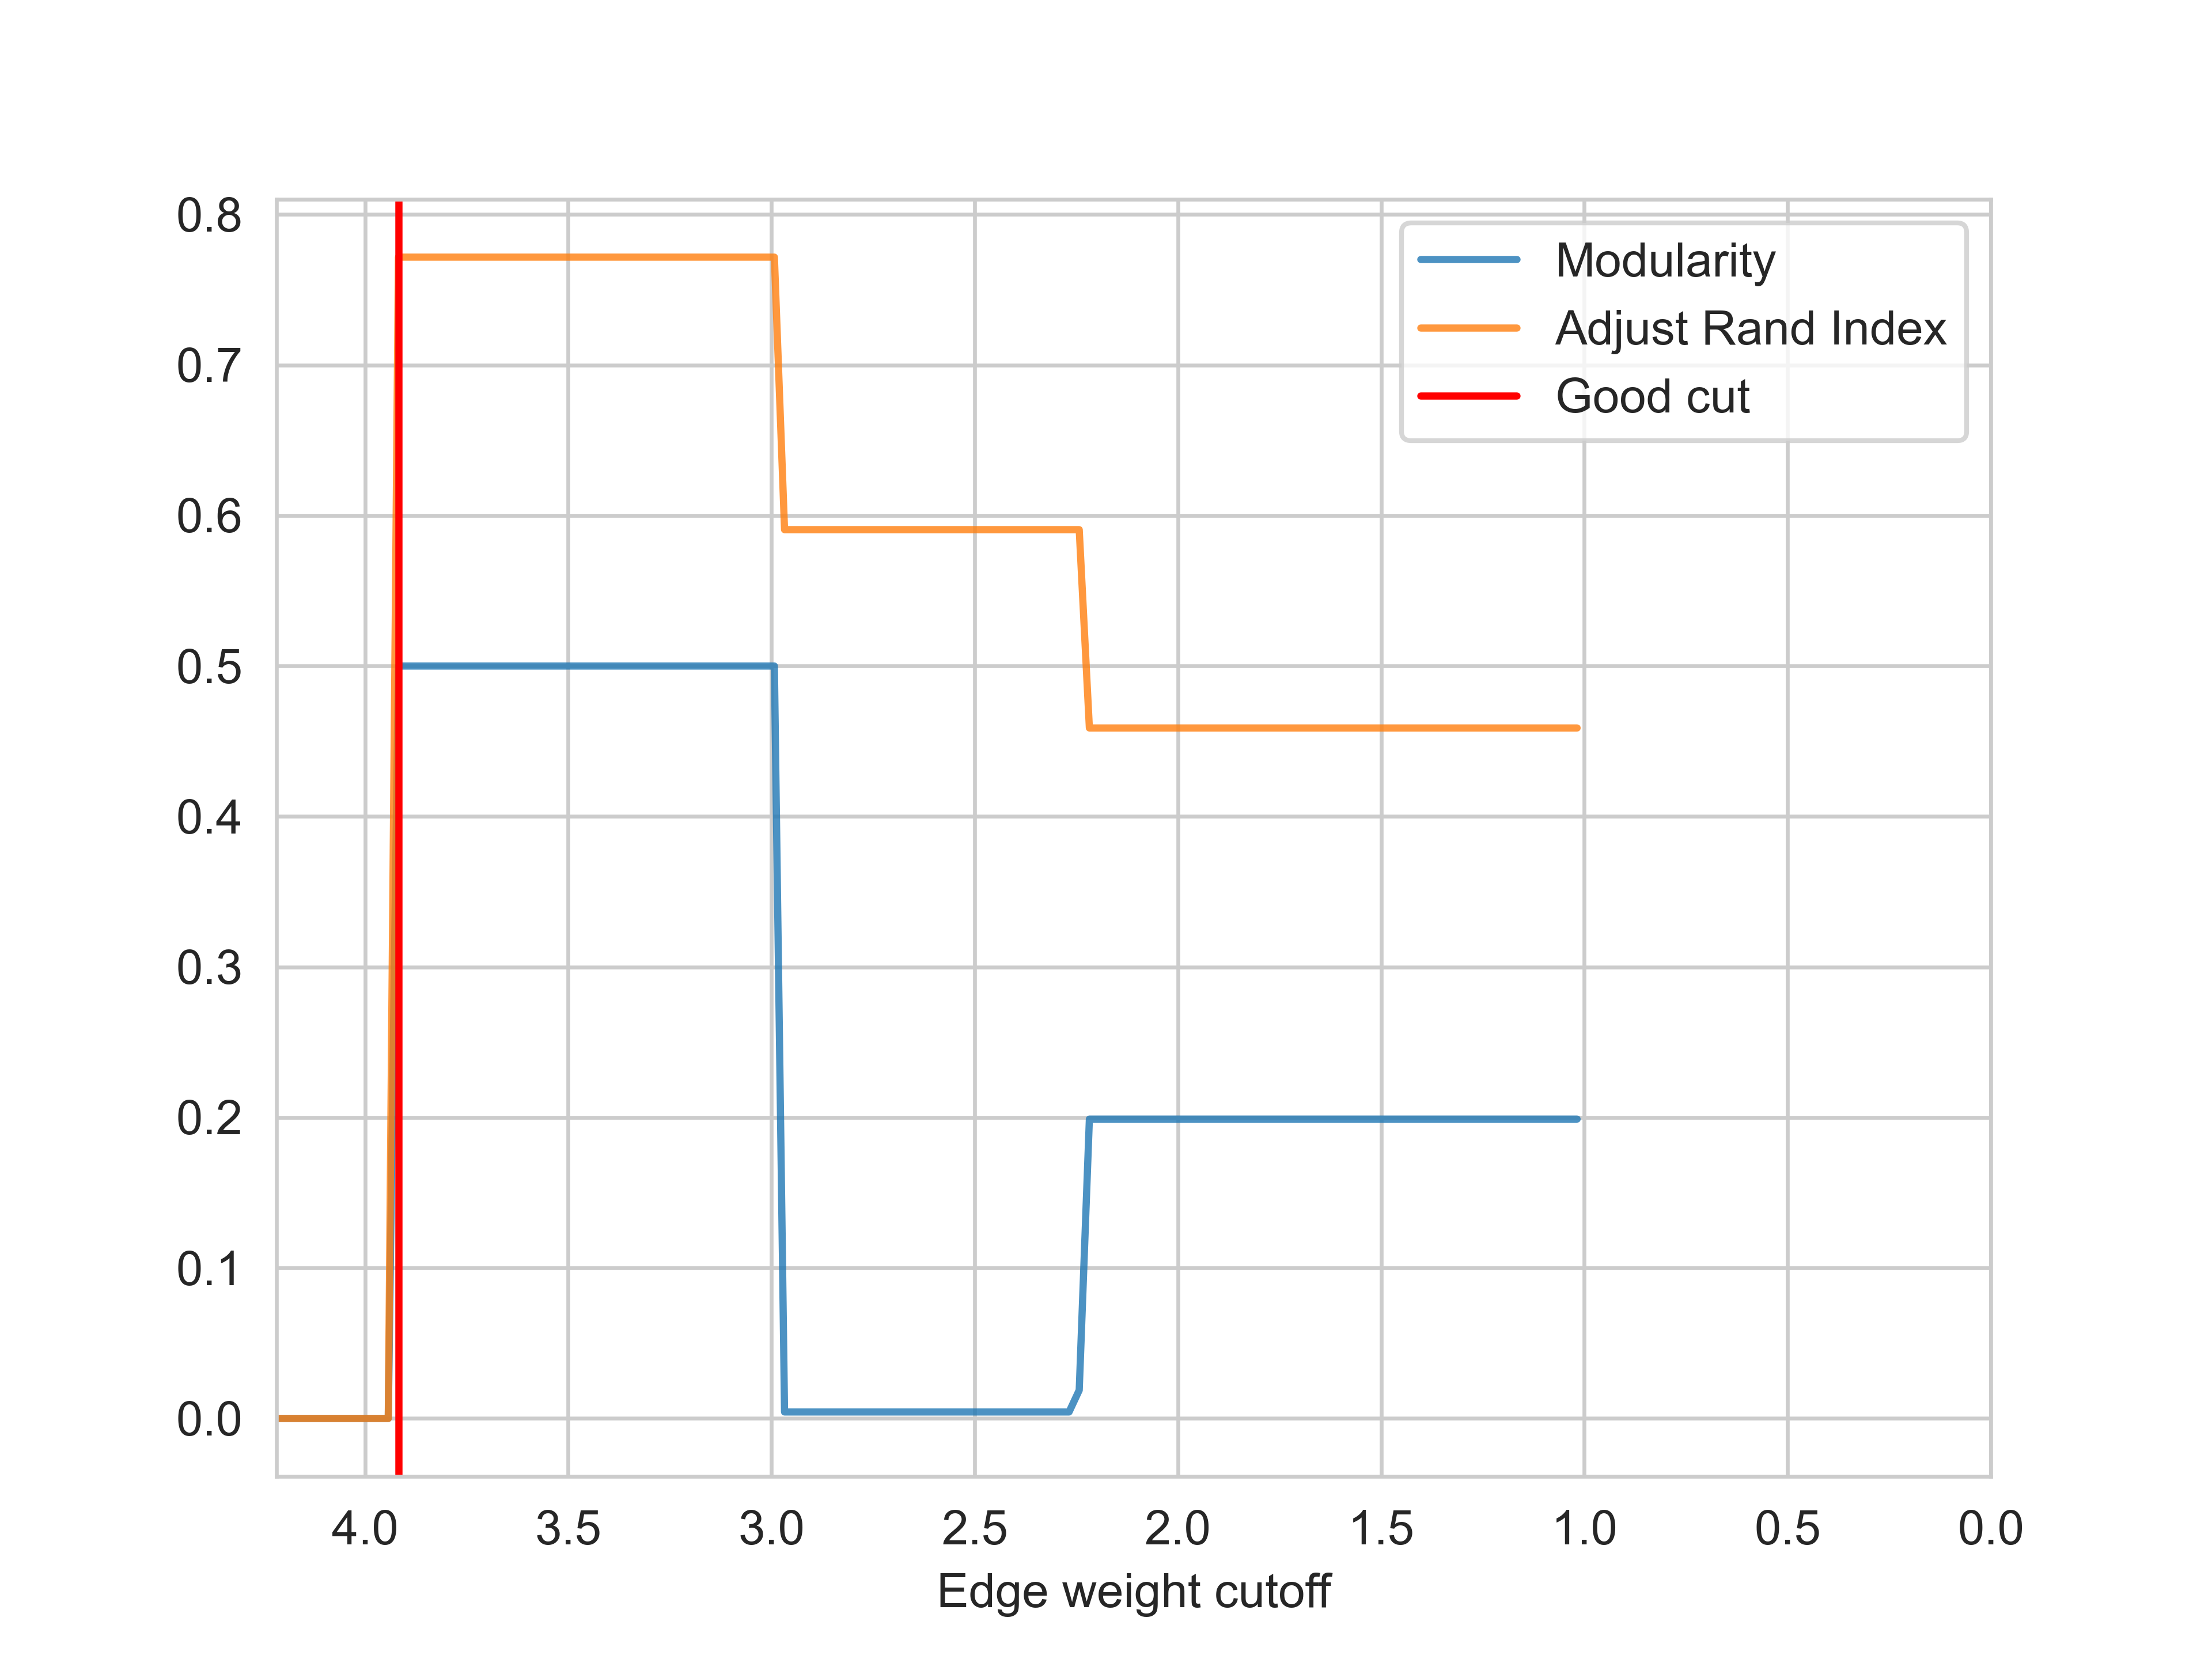
\includegraphics[width=0.6\textwidth]{../KarateClubResults/Surgery Accuracy.png}
    \caption{Karate acc}
    \label{fig:Karate_Accuracy}
\end{figure}

\begin{figure}
    \centering
    \begin{subfigure}{0.45\textwidth}
        \centering
        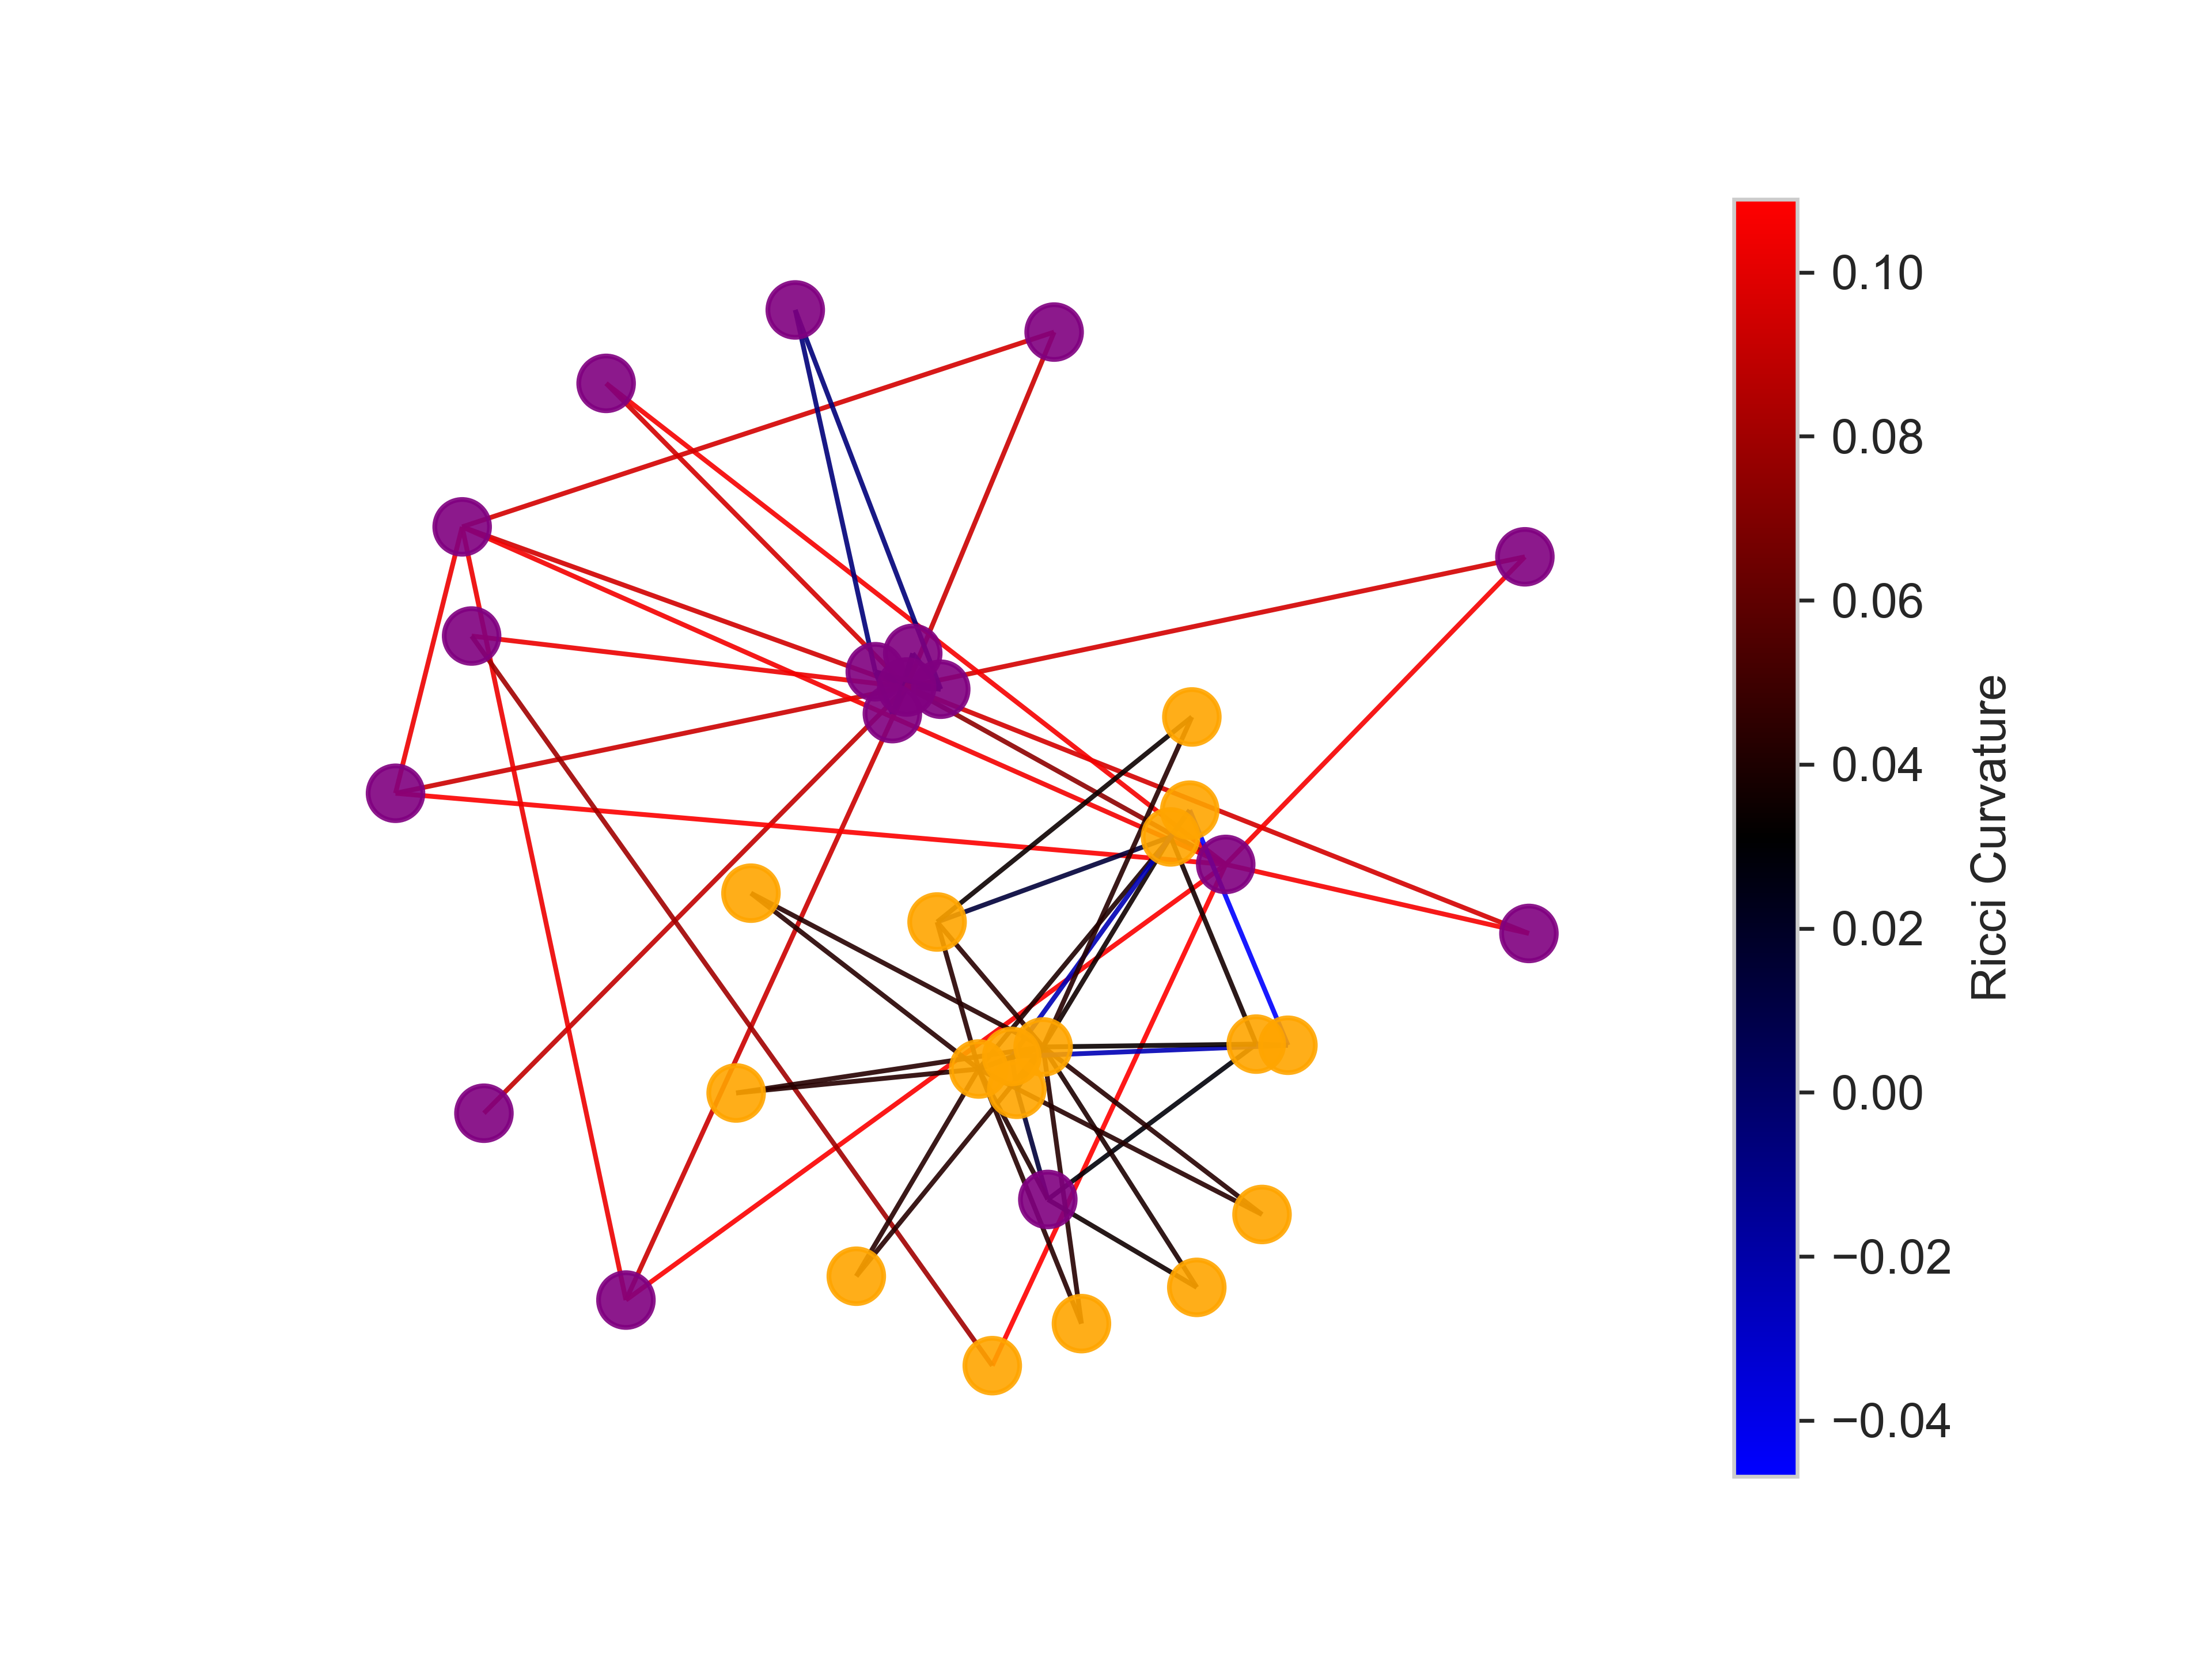
\includegraphics[width=\textwidth]{../KarateClubResults/After Surgery.png}
        \caption{Final Karate graph, after surgery process.}
        \label{fig:Karate_Surgery}
    \end{subfigure}
    \hfill
    \begin{subfigure}{0.45\textwidth}
        \centering
        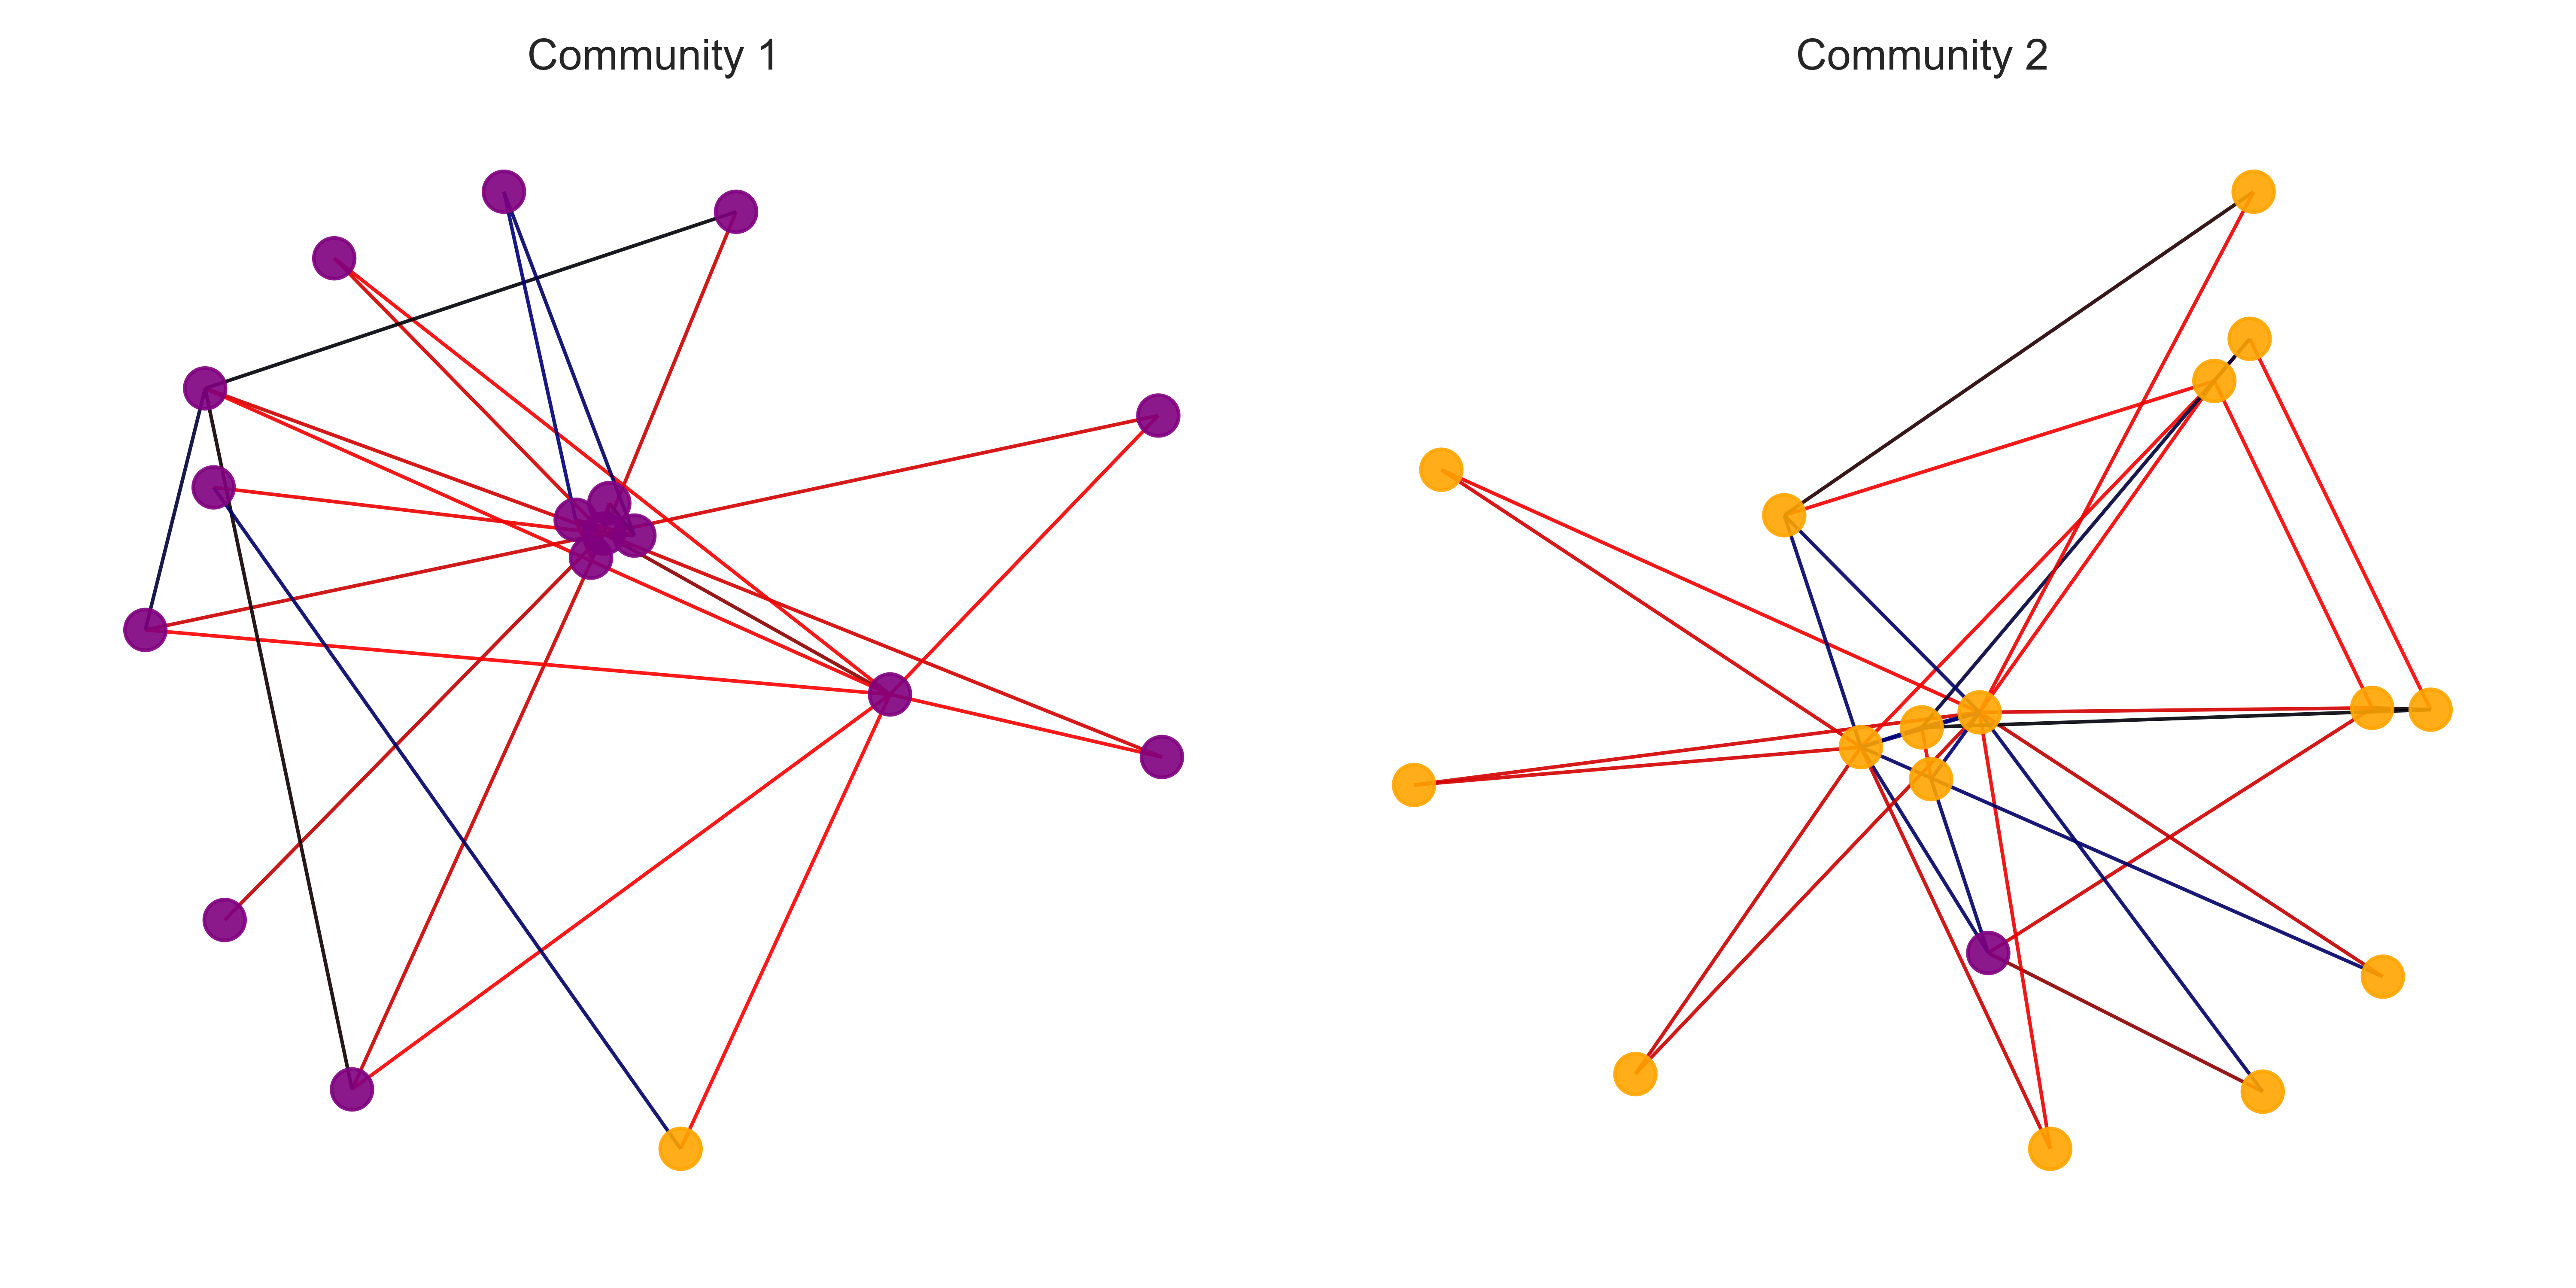
\includegraphics[width=\textwidth]{../KarateClubResults/Detected Communities.png}
        \caption{Detected communities after surgery on Karate graph.}
        \label{fig:Karate_Communities_Detected}
    \end{subfigure}
    \caption{Comparison of Karate graph after surgery and corrensponding connected components (i.e. the detected communities).}
    \label{fig:Karate_Communities}
\end{figure}

\begin{figure}
    \centering
    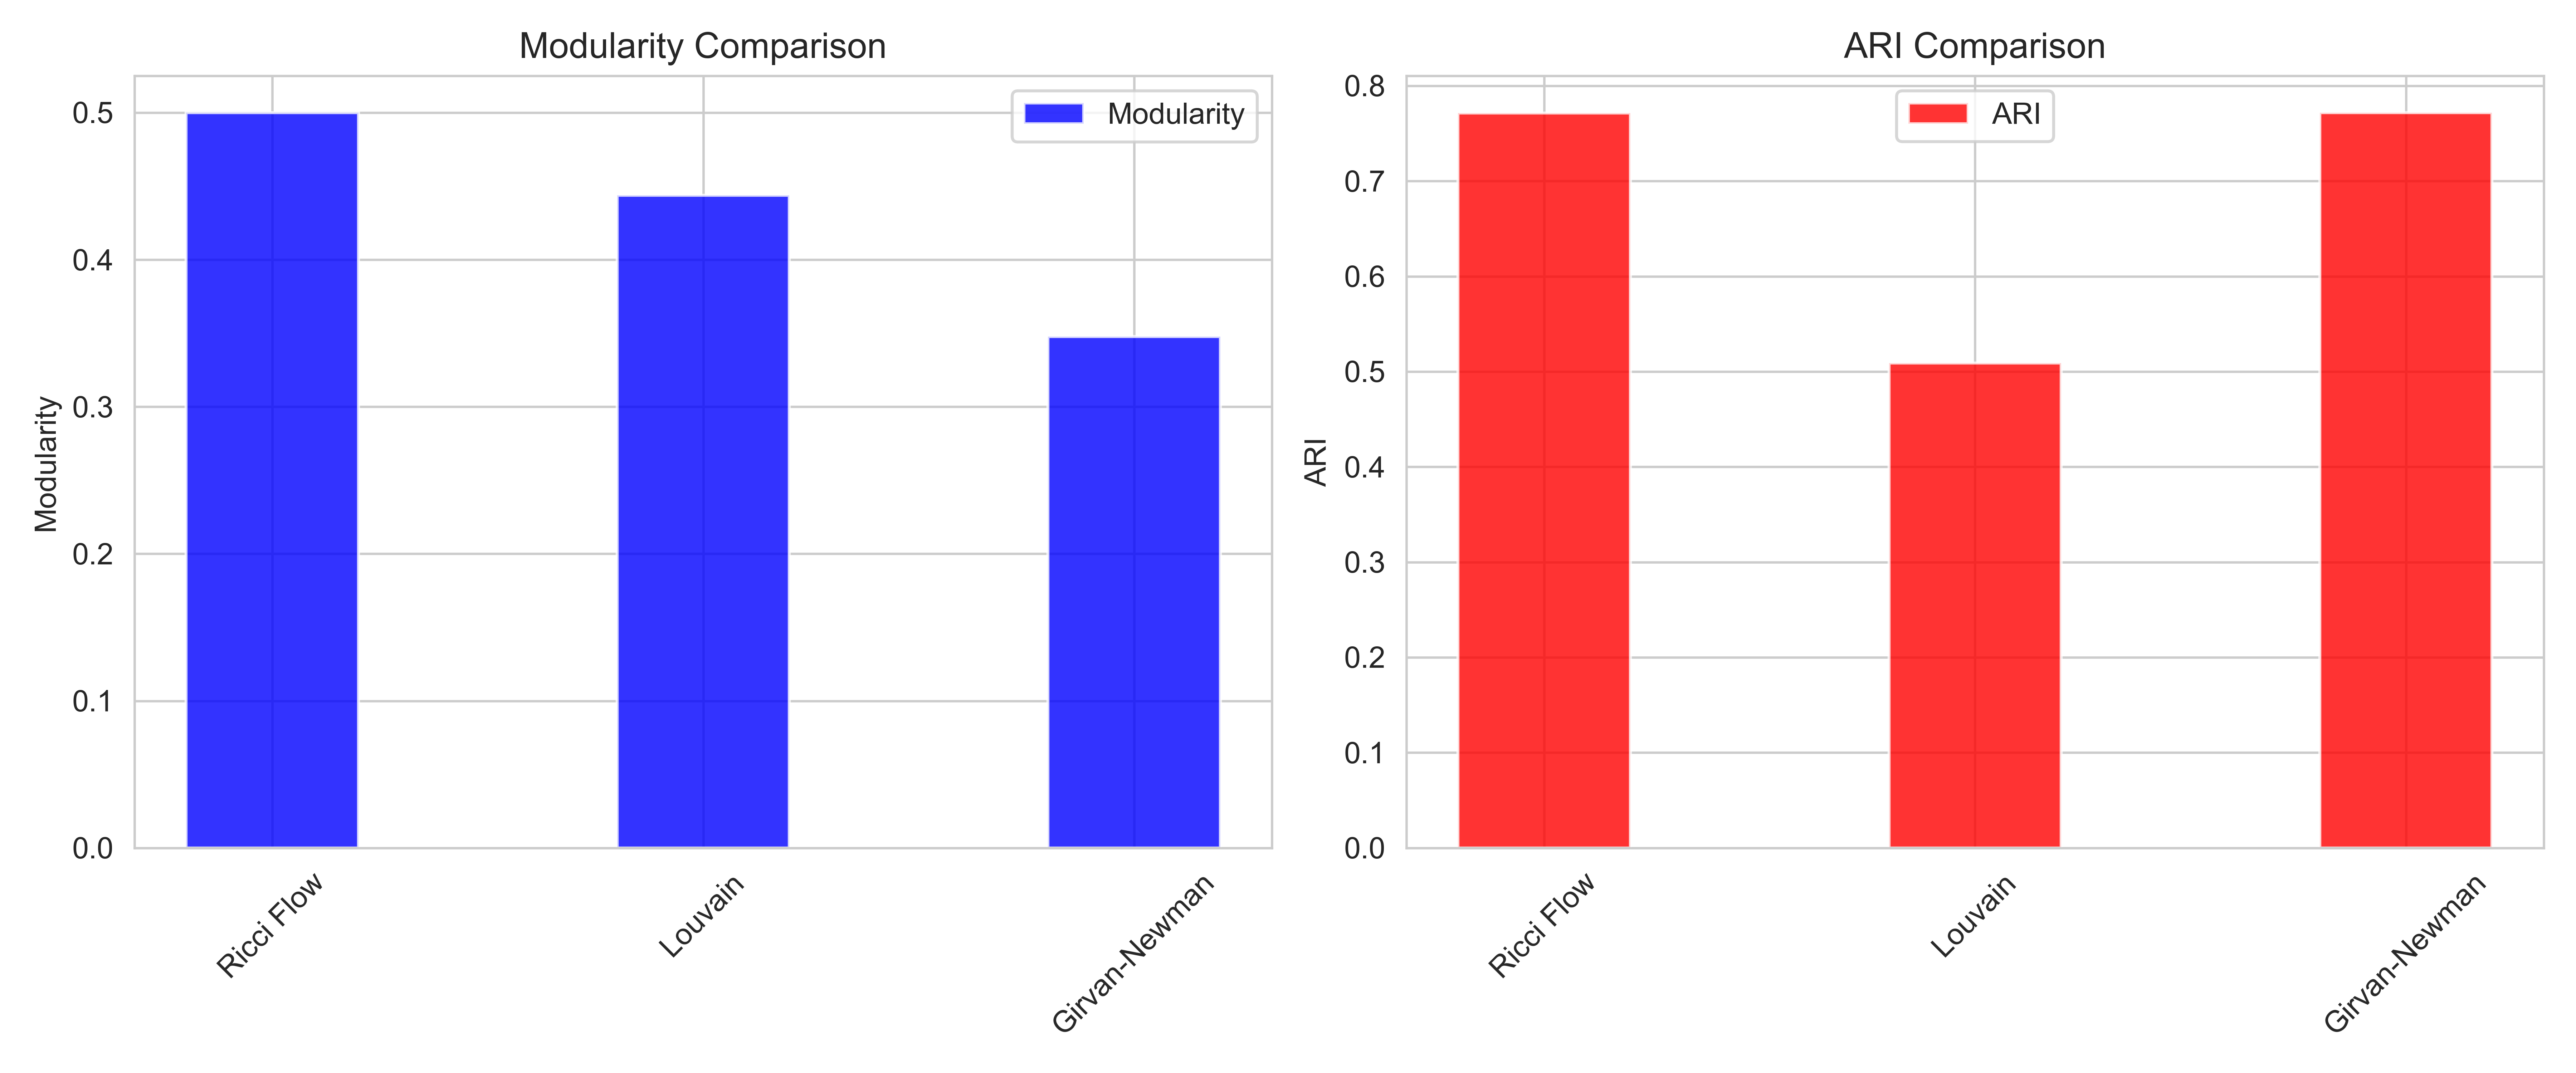
\includegraphics[width=0.6\textwidth]{../KarateClubResults/Comparison.png}
    \caption{Karate acc}
    \label{fig:Karate_Comparison}
\end{figure}
\chapter{Conclusions and Future Directions}

% ********************************** Appendices ********************************
\begin{appendices} % Using appendices environment for more functunality
\chapter{Metric of a 2-sphere}

%\section*{\hyperlink{Sphere}{Metric of a 2-sphere}} \label{appendix}
\begin{comment}
Start with the parameterisation of a 2-sphere with a radius $R$ and define the metric tensor $\eta$
\begin{equation*}
\centering
    \begin{cases}
      x = R \sin{(\theta)} \cos{(\phi)} \\
      y=  R \sin{(\theta)} \sin{(\phi)}\\
      z=  R \cos{(\theta)}
    \end{cases}
    \quad \text{and} \quad \eta_{ij} \equiv \begin{pmatrix}
\frac{\partial \Vec{x}}{\partial \theta} \frac{\partial \Vec{x}}{\partial \theta} & \frac{\partial \Vec{x}}{\partial \theta} \frac{\partial \Vec{x}}{\partial \phi} \\
\frac{\partial \Vec{x}}{\partial \phi}\frac{\partial \Vec{x}}{\partial \theta} & \frac{\partial \Vec{x}}{\partial \phi}\frac{\partial \Vec{x}}{\partial \phi} \\
\end{pmatrix}
\end{equation*}
\begin{equation*}
    \Rightarrow  \quad \eta_{ij}=\begin{pmatrix}
R^2 & 0 \\
0 & R^2 \sin^2(\theta) \\
\end{pmatrix}
\end{equation*}
where $\Vec{x}=\left( x , y , z \right)$. Now we can write the metric as
\begin{equation*}
    dl^2= \eta_{ij}\left( du^i , du^j \right) = R^2 \left( d\theta , d\phi \right) \begin{pmatrix}
1 & 0 \\
0 & \sin^2(\theta) \\
\end{pmatrix} \begin{pmatrix}
d\theta \\
d\phi \\
\end{pmatrix} = R^2 \left( d\theta^2 + \sin^2(\theta)d\phi^2 \right)
\end{equation*} 
where $\Vec{u}=(\theta,\phi)$.
\hspace*{\fill} $\Box$

\section*{\hyperlink{Ricci}{Components of the Ricci tensor for a generic spherically symmetric four dimensional metric}}
The explicit derivation will be shown only for the first component $R^0_0$, as the procedure is analogous for the others.

Starting from the expression of the Ricci tensor in terms of Christoffel symbols:
\begin{equation*}
    R^k {}_{\alpha k \beta} = \partial_\beta  \Gamma^k {}_{\alpha k} -\partial_k \Gamma^k {}_{\alpha \beta}+  \Gamma^\sigma {}_{\beta k} \Gamma^k {}_{\sigma \alpha}  -\Gamma^k {}_{k \sigma} \Gamma^\sigma {}_{\alpha \beta} 
\end{equation*}

we get 
\begin{align*}
    &R_{0 0} \equiv R^k {}_{0 k 0} =  \partial_0  \Gamma^k {}_{0 k}-\partial_k \Gamma^k {}_{0 0}  + \Gamma^\sigma {}_{0 k} \Gamma^k {}_{\sigma 0} - \Gamma^k {}_{k \sigma} \Gamma^\sigma {}_{0 0}   
\end{align*}

For the metric (\ref{eq2.1}), the terms that define $R_{00}$ are then expressed as
\begin{align*}
  \bullet \text{ } \Gamma^k {}_{0k} =& \partial_0 (\gamma + \alpha + 2\beta + \ln{\sin{\theta}}) = \Dot{\gamma} + \Dot{\alpha} +2\Dot{\beta} 
    \\ \rightarrow \quad \partial_0 \Gamma^k {}_{0k} =& \partial_0  (\Dot{\gamma} + \Dot{\alpha} +2\Dot{\beta})  = \Ddot{\gamma} + \Ddot{\alpha} +2\Ddot{\beta} \text{ ;}
    \\[15pt]  \bullet  \text{ } \Gamma^k {}_{0 0} =& \frac{1}{2} g^{k \nu} \left( g_{\nu 0 ,0} +  g_{\nu 0 ,0} -  g_{0 0,\nu} \right)= \frac{1}{2} g^{k\nu} \left(2g_{\nu 0,0}-g_{00,\nu}\right) 
  \\ =& \frac{1}{2}\left[ g^{k0}g_{0 0,0} + g^{k1}(2g_{0 1,0} - g_{0 0,1})\right] = \frac{1}{2}\left[ g^{k0}g_{0 0,0} - g^{k1} g_{0 0,1}\right] 
   \\ \rightarrow \quad \partial_k \Gamma^k {}_{00} =& \partial_0 \frac{1}{2}\left( e^{-2\gamma}2\dot{\gamma}e^{2\gamma}\right) - \partial_1 \frac{1}{2}\left(-e^{-2\alpha} 2\gamma^\prime e^{2\gamma}\right)
   \\ =& \Ddot{\gamma} + e^{2\gamma-2\alpha}\left(\gamma^{\prime \prime}+2{\gamma^\prime}^2 -2 \gamma^\prime \alpha^\prime \right) \text{;}
    \\[15pt]  \bullet \text{ } \Gamma^\sigma {}_{0 k} =& \frac{1}{2} g^{\sigma \nu} \left( g_{\nu 0, k} + g_{\nu k, 0} - g_{0 k, \nu}\right) 
    \\=& \frac{1}{2} \left[g^{\sigma 0} \left(  g_{0 0, k} + g_{0 k, 0} - g_{0 k, 0}\right) + g^{\sigma 1} \left( g_{1 0, k} + g_{1 k, 0} - g_{0 k, 1}\right) \right]
    \\ \Gamma^k {}_{\sigma 0} =& \frac{1}{2} g^{k \nu} \left( g_{\nu \sigma, 0} + g_{\nu 0,\sigma} - g_{\sigma 0, \nu}\right) 
    \\=& \frac{1}{2} \left[g^{k 0} \left( g_{0 \sigma, 0} + g_{0 0, \sigma} + - g_{\sigma 0, 0}\right) + g^{k 1}\left( g_{0 1, \sigma} + g_{\sigma 1, 0} - g_{\sigma 0, 1}\right) \right]
    \\ \rightarrow \quad \Gamma^\sigma {}_{0 k} \Gamma^k {}_{\sigma 0}  =& \Gamma^0 {}_{0 0} \Gamma^0 {}_{0 0} + \Gamma^0 {}_{0 1} \Gamma^1 {}_{0 0} + \cancel{\Gamma^0 {}_{0 2} \Gamma^2 {}_{0 0}} + \cancel{\Gamma^0 {}_{0 3} \Gamma^3 {}_{0 0}} + \Gamma^1 {}_{0 0} \Gamma^0 {}_{1 0} + \Gamma^1 {}_{0 1} \Gamma^1 {}_{1 0} 
    \\ +&\cancel{\Gamma^1 {}_{0 2} \Gamma^2 {}_{1 0}} + \cancel{\Gamma^1 {}_{0 3} \Gamma^3 {}_{1 0}} + \cancel{\Gamma^2 {}_{0 0} \Gamma^0 {}_{2 0}} + \cancel{\Gamma^2 {}_{0 1} \Gamma^1 {}_{2 0}} + \Gamma^2 {}_{0 2} \Gamma^2 {}_{2 0} + \cancel{\Gamma^2 {}_{0 3} \Gamma^3 {}_{2 0}} 
    \\ +&\cancel{\Gamma^3 {}_{0 0} \Gamma^0 {}_{3 0}} + \cancel{\Gamma^3 {}_{0 1} \Gamma^1 {}_{3 0}} + \cancel{\Gamma^3 {}_{0 2} \Gamma^2 {}_{3 0}}  + \Gamma^3 {}_{0 3} \Gamma^3 {}_{3 0} 
    \\ =& \Dot{\gamma}^2 + {\gamma^\prime}^2 e^{2\gamma-2\alpha} + {\gamma^\prime}^2 e^{2\gamma-2\alpha}+ \Dot{\alpha}^2 + \Dot{\beta}^2 + \Dot{\beta}^2
    \\ =& \dot{\gamma}^2 + \dot{\alpha}^2 + 2 \dot{\beta}^2 + 2{\gamma^\prime}^2 e^{2\gamma-2\alpha} \text{ ;}
    \\[15pt]  \bullet \text{ } \Gamma^\sigma 
    {}_{0 0} =&  \frac{1}{2} g^{\sigma \nu}(2g_{\nu 0,0} - g_{00,\nu})  
    = \frac{1}{2} \left[ g^{\sigma 0}g_{00,0} -g^{\sigma 1}g_{00,1}\right]
    \\ \Gamma^k {}_{k \sigma} =& \partial_\sigma (\gamma + \alpha +2\beta + \ln{\sin{\theta}})
    \\ \rightarrow \quad  \Gamma^k {}_{k \sigma} \Gamma^\sigma {}_{0 0} =& \frac{1}{2} e^{-2\gamma}\left(2 \Dot{\gamma}e^{2\gamma}\right)  \left(\Dot{\gamma} + \Dot{\alpha} +2\Dot{\beta} \right) - \frac{1}{2} e^{-2\alpha}\left(- 2 \gamma^\prime e^{2\gamma}\right)  \left(\gamma^\prime +\alpha^\prime +2\beta^\prime \right)
    \\ =&\dot{\gamma}^2 + \dot{\gamma}\Dot{\alpha} + 2\dot{\gamma}\Dot{\beta} + e^{2\gamma-2\alpha}\left({\gamma^\prime}^2+ \gamma^\prime \alpha^\prime + 2\gamma^\prime \beta^\prime \right)
\end{align*}
where dots and primes stand for $\frac{\partial}{\partial t}$ and  $\frac{\partial}{\partial r}$, respectively. 
In the computation we made use of two important relationships that hold in the case of a symmetric connection: 
\begin{equation*}
    \Gamma^\mu {}_{\alpha \beta} = \frac{1}{2} g^{\mu \nu} \left( g_{\nu \alpha,\beta} + g_{\nu \beta,\alpha} -  g_{\alpha \beta,\nu} \right) \quad \text{and} \quad \Gamma^\alpha {}_{\mu \alpha} = \Gamma^\alpha {}_{\alpha \mu} = \partial_\mu \left( \ln{\sqrt{-g}}\right)
\end{equation*}
Where the term $\ln{\sqrt{-g}} \equiv \ln{\sqrt{-\det g_{\mu \nu}}}$ evaluates as
\begin{align*}
    g  &= -e^{2\gamma + 2\alpha +4\beta}\sin^2{\theta}
    \\ \sqrt{-g} &= e^{\gamma + \alpha +2\beta}\sin{\theta}
    \\ \ln{\sqrt{-g}} &=\gamma + \alpha +2\beta + \ln{\sin{\theta}}
\end{align*}

We are now able to write
\begin{align*}
    R_{00} =& \text{ } \Ddot{\gamma} + \Ddot{\alpha} + 2\Ddot{\beta} - \Ddot{\gamma} - e^{2\gamma-2\alpha}\left(\gamma^{\prime \prime}+2{\gamma^\prime}^2 -2 \gamma^\prime \alpha^\prime \right) + \dot{\gamma}^2 + \dot{\alpha}^2 + 2 \dot{\beta}^2 + {\gamma^\prime}^2 e^{2\gamma-2\alpha}
    \\ -& \dot{\gamma}^2 - \dot{\gamma}\Dot{\alpha} - 2\dot{\gamma}\Dot{\beta} 
     - e^{2\gamma-2\alpha}\left({\gamma^\prime}^2+ \gamma^\prime \alpha^\prime + 2\gamma^\prime \beta^\prime \right)
    \\ =& \text{ } \Ddot{\alpha} + 2\Ddot{\beta} + 2 \dot{\beta}^2  -
    \Dot{\gamma} \left( \Dot{\alpha} + 2\Dot{\beta} \right) + \dot{\alpha}^2 - e^{2\gamma-2\alpha}\left( \gamma^{\prime \prime} - \gamma^\prime \alpha^\prime + {\gamma^\prime}^2 + 2\gamma^\prime \beta^\prime\right)
\end{align*}
To obtain $R^0_0$ we use the relationship $R^0_0=g^{0 0}R_{0 0}$, where $g^{0 0} = e^{-2\gamma}$. 
\begin{equation*}
    R^0_0=e^{-2\gamma}\left[ 2 \Ddot{\beta} + \Ddot{\alpha} + 2 \dot{\beta}^2 + \dot{\alpha}^2 - \dot{\gamma} \left( 2 \dot{\beta} + \dot{\alpha} \right) \right] - e^{-2 \alpha}\left[ \gamma^{\prime \prime} + \gamma^{\prime} \left( 2 \beta^\prime + \gamma^\prime - \alpha^\prime \right) \right]
\end{equation*}
\hspace*{\fill} $\Box$
\end{comment}
\end{appendices}

% ********************************** Back Matter *******************************
% Backmatter should be commented out, if you are using appendices after References
\backmatter

% ********************************** Bibliography ******************************
\begin{spacing}{0.9}

\cleardoublepage
\nocite{*}
\printbibliography[heading=bibintoc, title={References}]

\end{spacing}

% ******************************************************************************
% ******************************** END DOCUMENT ********************************
% ******************************************************************************

\end{document}